\documentclass[11pt]{report}

\usepackage{epsf,amsmath,amsfonts}
\usepackage{graphicx}
\usepackage{longtable}
\usepackage{hyperref}
\usepackage{color}
\usepackage{calc}
\usepackage{url}
\usepackage{xstring}

\setlength{\topmargin}{0in}
\setlength{\headheight}{0in}
\setlength{\headsep}{0in}
\setlength{\textheight}{9.0in}
\setlength{\textwidth}{6.5in}
\setlength{\evensidemargin}{0in}
\setlength{\oddsidemargin}{0in}

\setlength\LTleft\parindent
\setlength\LTright\fill

\newcommand{\version}{5.0}
\newcommand{\core}{atmosphere}

\hypersetup{
    colorlinks=true,
    linkcolor=red
}


% Thanks, StackExchange!
% http://tex.stackexchange.com/questions/20890/define-an-escape-underscore-environment
\DeclareUrlCommand\UScore{\urlstyle{rm}}

\newcommand{\namelist}[1]{\hyperlink{#1}{\StrDel{#1}{mnl:}[\outrec]\StrDel{\outrec}{inl:}[\outrec]\StrSubstitute{\outrec}{_}{\_}}}
\newcommand{\namelistrecord}[1]{\hyperlink{#1}{\StrDel{#1}{mrec:}[\outrec]\StrDel{\outrec}{irec:}[\outrec]\&\StrSubstitute{\outrec}{_}{\_}}}
\newcommand{\field}[1]{\hyperlink{#1}{\UScore{#1}}}

\begin{document}

\title{\bf \hfil MPAS-Atmosphere Model User's Guide \hfil \break \hfil \break Version \version}

%\author{\bf Version \version}

\maketitle

\chapter*{Foreword}
\label{chap:foreword}

This user's guide describes the Model for Prediction Across Scales -- Atmosphere
(MPAS-A) Version \version.   MPAS-A is the non-hydrostatic atmosphere model built within the MPAS
framework. Users guides for other MPAS components, such as MPAS-Ocean, are separate from this guide.

The component models and framework that comprise MPAS are being developed collaboratively between Los Alamos National
Laboratory (LANL) and the National Center for Atmospheric Research (NCAR).
Common functionality required by different MPAS component models, such as parallel
input/output, time management, block decomposition, etc., is provided by the
MPAS framework, while development of specific component models, referred to in MPAS as {\em cores}, is handled by the
individual development groups.  Currently, LANL is responsible for the ocean core and the land-ice core, and NCAR is responsible for the atmospheric core, MPAS-A.

MPAS is very much a collaborative development of both the shared architectures and the component models.  There are a number of contributors to the developments leading to the MPAS-A solver, and many of these developments are shared with the ocean core.  The C-grid Voronoi discretization is based on critical developments from John Thuburn, Todd Ringler, Bill Skamarock, and Joe Klemp.  The mesh generation that enables the MPAS-A development received major contributions from Todd Ringler, Doug Jacobson, Max Gunzburger, and Lili Ju.  Significant developments in the transport scheme were accomplished by Bill Skamarock and Almut Gassmann.  The atmospheric physics has been taken from the Advanced Research WRF model; these physics have benefitted from the work of hundreds of scientists.  On the framework side we leverage a number of outside packages that have received extensive development from a wide community, including NetCDF (UCAR/Unidata) and PIO (as used in the Community Earth Systems Model, CESM).

The software developed for MPAS is open source, and it has been copyrighted under a BSD license.  The simple copyright statement can be found at the beginning of MPAS source files and the complete copyright statement can be found in this user's guide or in the `LICENSE' file accompanying the source code.

We conclude by noting that this user's guide is a work in progress.  We welcome suggestions for improvements to this guide, including additions, corrections, clarifications, etc.  Updates to MPAS-A, including the most recent code,
user's guide, and test cases, may be found at \hfil\break \url{http://mpas-dev.github.com}.

\vspace{8pt}
\noindent
{\bf Contributors to this guide:}\\
Michael Duda, Laura Fowler, Bill Skamarock, Conrad Roesch, Doug Jacobsen, and Todd Ringler.


%\vspace{8pt}
\vfil
\noindent
{\it The National Center for Atmospheric Research (NCAR) is operated by the
University Corporation for Atmospheric Research (UCAR) and is sponsored by the
National Science Foundation.  Any opinions, findings, conclusions, or
recommendations expressed in this publication are those of the authors and do
not necessarily reflect the views of the National Science Foundation.}


\tableofcontents

%--------------------------------------------------------------------------------------------
% MPAS-A Overview
%--------------------------------------------------------------------------------------------

\chapter{MPAS-Atmosphere Overview}
\label{chap:atmosphere_overview}

The Model for Prediction Across Scales -- Atmosphere (MPAS-A) is a
non-hydrostatic atmosphere model that is part of a family of
Earth-system component models collectively known as MPAS.  All MPAS
models have in common their use of centroidal Voronoi tessellations for
their horizontal meshes, which has motivated the development of a common
software framework that provides a high-level driver program and
infrastructure for providing parallel execution, input and output, and
other software infrastructure.

\section{Features}

Important features of MPAS-A include:

\begin{itemize}
\item Fully-compressible, non-hydrostatic dynamics
\item Split-explicit Runge-Kutta time integration
\item Exact conservation of dry-air mass and scalar mass
\item Positive-definite and monotonic transport options
\item Generalized terrain-following height coordinate
\item Support for unstructured variable-resolution (horizontal) mesh integrations for the sphere and Cartesian planes.
\end{itemize}

At present, MPAS-A includes parameterizations of physical processes
taken from the Weather Research and Forecasting (WRF) Model
\footnote{\url{http://www.wrf-model.org/}.}. Specifically, MPAS-A has
support for:

\begin{itemize}
\item Radiation: CAM and RRTMG long-wave and short-wave radiation schemes
\item Land-surface: NOAH land-surface model
\item Surface-layer: Monin-Obukhov and MYNN
\item Boundary-layer: YSU and MYNN PBL schemes
\item Convection: Kain-Fritsch Tiedtke, New Tiedtke, and Grell-Freitas convection parameterizations
\item Cloud microphysics: WSM6, Kessler, and Thompson schemes
\end{itemize}

\section{Model components}

MPAS-A is comprised of two main components: the model, which includes
atmospheric dynamics and physics; and an initialization component for
generating initial conditions for the atmospheric and land-surface state as well as update files for sea-surface
temperature and sea ice. Both components (model and initialization) are built as {\it cores}
within the MPAS software framework and make use of the same driver
program and software infrastructure.  However, each component is compiled as
a separate executable.

\begin{figure}[htb]
\begin{center}
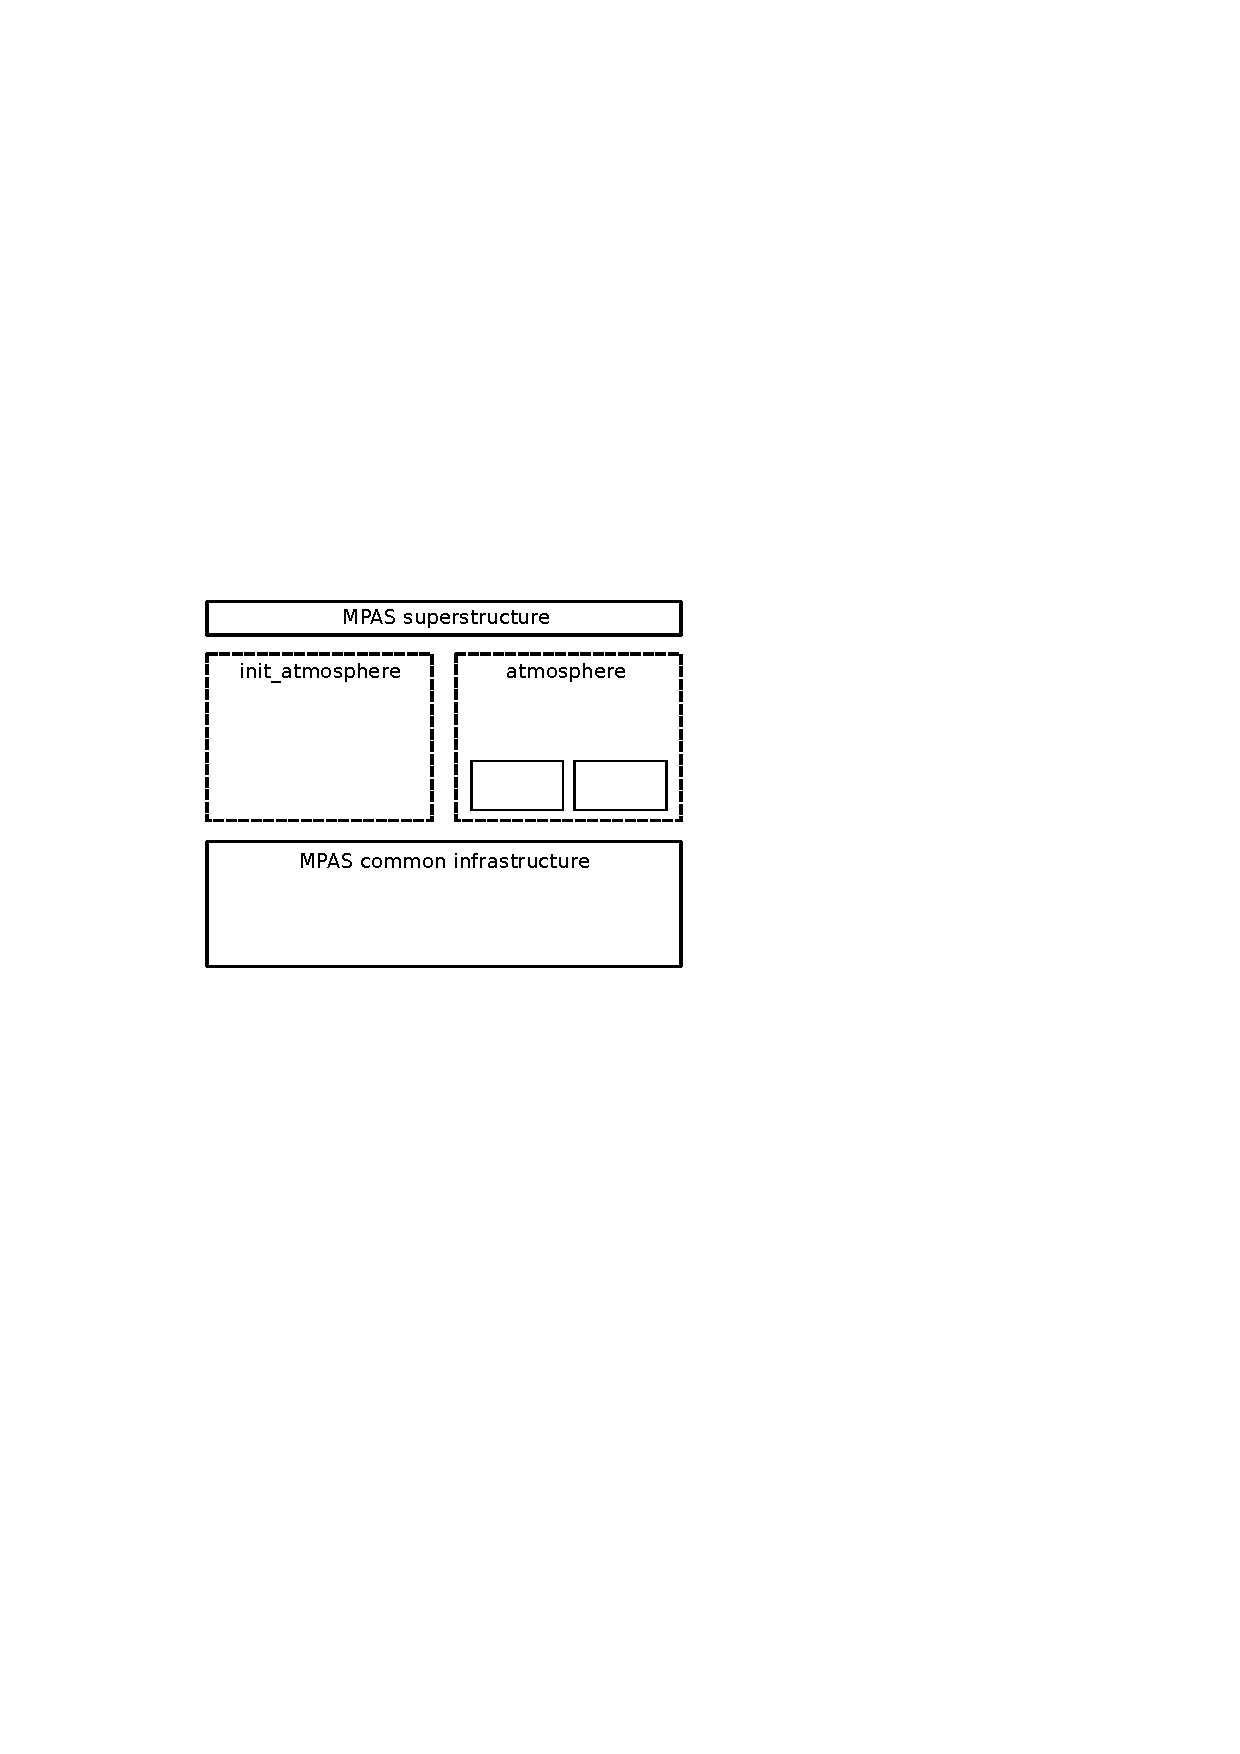
\includegraphics[width=3.5in]{figures/mpas-a_components.pdf}
\caption{The initialization and model components of MPAS-A are built as
separate {\em cores} within the MPAS framework.}
\label{fig:atm_components}
\end{center}
\end{figure}

A succinct description of building and running MPAS-A is given in Chapter \ref{chap:quick_start}, the Quick Start Guide.
Detailed instructions for building these components are given in Chapter
\ref{chap:mpas_build_instructions}, and the basic steps to create initial
conditions and run the MPAS-A model are outlined in Chapter
\ref{chap:running_mpas_a}.

\chapter{MPAS-Atmosphere Quick Start Guide}
\label{chap:quick_start}

This chapter provides MPAS-Atmosphere users with a quick start description of
how to build and run the model. It is meant merely as a brief overview of the
process, while the more detailed descriptions of each step are provided in later
chapters.

In general, the build process follows the following steps.

\begin{enumerate}
	\item Build MPI Layer (OpenMPI, MVAPICH2, etc; Section \ref{build_prerequisites})
	\item Build serial NetCDF library (v3.6.3, v4.1.3, etc; Section \ref{serial_netcdf})
	\item Build Parallel-NetCDF library (v1.2.1, v1.3.0, etc; Section \ref{parallel_netcdf})
	\item Build Parallel I/O library (v1.4.1, v1.6.1, etc; Section \ref{pio_build})
	\item Build METIS library and executables (v4.0, v5.0.2, etc; Section \ref{sec:metis})
	\item Checkout MPAS-Atmosphere from repository
	\item Build init\_atmosphere and atmosphere cores; Section \ref{compiling_MPAS}
\end{enumerate}

After completing these steps, executable files named {\tt init\_atmosphere\_model} and
{\tt atmosphere\_model} should have been created in the top-level MPAS directory. Once
both executables have been created, one can begin the run process as follows:

\begin{enumerate}
	\item Create run directory.
	\item Copy executables to run directory.
	\item Copy namelist.input, input and graph files into run directory. 
	\item Edit namelist.input to have the proper parameters.
	\item (Optional) Create graph files, using METIS executable (pmetis or gpmetis depending on version).  A graph file is required for each processor count you want to use.
	\item Run MPAS-Atmosphere (e.g.\ {\tt mpirun -np 8 atmosphere\_model}).
	\item Visualize output, and perform analyses.
\end{enumerate}

\chapter{Building MPAS}
\label{chap:mpas_build_instructions}

\section{Prerequisites}
\label{build_prerequisites}

To build MPAS, compatible C and Fortran compilers are required. Additionally,
the MPAS software relies on the PIO parallel I/O library to read and write model
fields, and the PIO library requires the standard netCDF library as well as the
parallel-netCDF library from Argonne National Laboratory. All libraries must be
compiled with the same compilers that will be used to build MPAS. Section
\ref{sec:build_io} summarizes the basic procedure of installing the required I/O
libraries for MPAS.

In order for the MPAS makefiles to find the PIO, parallel-netCDF, and netCDF
include files and libraries, the environment variables {\tt PIO}, {\tt PNETCDF},
and {\tt NETCDF} should be set to the root installation directories of the PIO,
parallel-netCDF, and netCDF installations, respectively. 

An MPI installation such as MPICH or OpenMPI is also required, and there is no
option to build a serial version of the MPAS executables. MPAS-Atmosphere v5.0
introduces the capability to use hybrid parallelism using MPI and OpenMP; however,
the use of OpenMP {\em should be considered experimental} and generally does not
offer any performance advantage. The primary reason for releasing a shared-memory
capability is to make this code available to collaborators for future development.


\section{Compiling I/O Libraries}
\label{sec:build_io}

{\bf IMPORTANT NOTE:} {\em The instructions provided in this section for
installing libraries have been successfully used by MPAS developers, but due to
differences in library versions, compilers, and system configurations, it is
recommended that users consult documentation provided by individual library
vendors should problems arise during installation. The MPAS developers cannot assume
responsibility for third-party libraries.} \vspace{12pt}

Although most recent versions of the netCDF and parallel-netCDF libraries should work,
the most tested versions of these libraries are netCDF 4.4.x and parallel-netCDF 1.8.x.
Users are strongly encouraged to use either the latest PIO 2.x version from \url{https://github.com/NCAR/ParallelIO/},
or PIO versions 1.7.1 or 1.9.23, as other versions have not been tested or are known to not work with MPAS.
The netCDF and parallel-netCDF libraries must be installed before building the PIO library.

\subsection{NetCDF}
\label{serial_netcdf}

Version 4.4.x of the netCDF library may be downloaded from
\url{http://www.unidata.ucar.edu/downloads/netcdf/index.jsp}.
The Unidata page provides detailed instructions instructions for building the netCDF C and Fortran libraries;
both the C and Fortran interfaces are needed by PIO. If netCDF-4 support is desired, the zlib and HDF5 libraries
will need to be installed prior to building netCDF. {\em Before proceeding to compile PIO
the {\tt NETCDF} environment variable should be set to the netCDF root
installation directory.}

\subsection{Parallel-NetCDF}
\label{parallel_netcdf}

Version 1.8.x of the parallel-netCDF library may be downloaded from
\url{https://trac.mcs.anl.gov/projects/parallel-netcdf/wiki/Download}. {\em Before proceeding to
compile PIO the {\tt PNETCDF} environment variable should be set to the
parallel-netCDF root installation directory.}

\subsection{PIO}
\label{pio_build}

Beginning with the MPAS v5.2 release, the either of the PIO 1.x or 2.x library versions
may be used. The two major versions have slightly different APIs; by default, the MPAS build
system assumes the PIO 1.x API, but the PIO 2.x library versions may be used by
adding the {\tt USE\_PIO2=true} option when compiling MPAS as described in Section \ref{compiling_MPAS}.
If compiling with the PIO 1.x library versions, users are strongly encouraged to choose
either PIO 1.7.1 or PIO 1.9.23, as other 1.x versions may not work; these two specific versions may
be obtained from \url{https://github.com/NCAR/ParallelIO/releases/tag/pio1_7_1} and
\url{https://github.com/NCAR/ParallelIO/releases/tag/pio1_9_23}.

The PIO 2.x library versions support integrated performance timing with the GPTL library; however,
the MPAS infrastructure does not currently provide calls to initialize this library when it is used in PIO 2.x.
Therefore, it is recommended to add {\tt -DPIO\_ENABLE\_TIMING=OFF} when running the cmake command
to build PIO 2.x versions.

After PIO is built and installed the {\tt PIO} environment variable should be set to 
the directory where PIO was installed. Recent versions of PIO support the specification of an installation
prefix, while some older versions do not, in which case the {\tt PIO} environment variable should
be set to the directory where PIO was compiled.

\section{Compiling MPAS}
\label{compiling_MPAS}

{\bf IMPORTANT NOTE:} {\em Before compiling MPAS, the {\tt NETCDF}, {\tt
PNETCDF}, and {\tt PIO} environment variables must be set to the library
installation directories as described in the previous section.} \vspace{12pt}

The MPAS code uses only the `make' utility for compilation. Rather than
employing a separate configuration step before building the code, all
information about compilers, compiler flags, etc., is contained in the top-level
{\tt Makefile}; each supported combination of compilers (i.e., a configuration)
is included in the {\tt Makefile} as a separate make target, and the user
selects among these configurations by running {\tt make} with the name of a
build target specified on the command-line, e.g.,

\vspace{12pt}
{\tt > make gfortran}
\vspace{12pt}

\noindent to build the code using the GNU Fortran and C compilers. Some of the
available targets are listed in the table below, and additional targets can be
added by simply editing the {\tt Makefile} in the top-level directory.

\vspace{12pt}
\begin{longtable}{| l | l | l | l |}
\hline
Target & Fortran compiler & C compiler & MPI wrappers \\ \hline \hline
{\tt xlf} & xlf90 & xlc & mpxlf90 / mpcc \\ \hline
{\tt pgi} & pgf90 & pgcc & mpif90 / mpicc \\ \hline
{\tt ifort} & ifort & gcc & mpif90 / mpicc \\ \hline
{\tt gfortran} & gfortran & gcc & mpif90 / mpicc \\ \hline
{\tt llvm} & flang & clang & mpifort / mpicc \\ \hline
{\tt bluegene} & bgxlf95\_r & bgxlc\_r & mpxlf95\_r / mpxlc\_r \\ \hline
\end{longtable}
\vspace{12pt}

The MPAS framework supports multiple {\em cores} --- currently a shallow water
model, an ocean model, a land-ice model, a non-hydrostatic atmosphere model, and
a non-hydrostatic atmosphere initialization core --- so the build process must be told which core
to build. This is done by either setting the environment variable {\tt CORE} to
the name of the model core to build, or by specifying the core to be built
explicitly on the command-line when running {\tt make}. For the atmosphere
core, for example, one may run either

\vspace{12pt}
{\tt > setenv CORE atmosphere}

{\tt > make gfortran}
\vspace{12pt}

\noindent or

\vspace{12pt}
{\tt > make gfortran CORE=atmosphere}
\vspace{12pt}

If the {\tt CORE} environment variable is set and a core is specified on the
command-line, the command-line value takes precedence; if no core is specified,
either on the command line or via the {\tt CORE} environment variable, the build
process will stop with an error message stating such.  Assuming compilation is
successful, the model executable, named {\tt \$\{CORE\}\_model} (e.g., {\tt
atmosphere\_model}), should be created in the top-level MPAS directory.

In order to get a list of available cores, one can simply run the top-level {\tt
Makefile} without setting the {\tt CORE} environment variable or passing the
core via the command-line. An example of the output from this can be seen
below.

{\small
\begin{verbatim}
> make
( make error )
make[1]: Entering directory `/scratch/MPAS-Release'

Usage: make target CORE=[core] [options]

Example targets:
    ifort
    gfortran
    xlf
    pgi

Availabe Cores:
    atmosphere
    init_atmosphere
    landice
    ocean
    seaice
    sw
    test

Available Options:
    DEBUG=true    - builds debug version. Default is optimized version.
    USE_PAPI=true - builds version using PAPI for timers. Default is off.
    TAU=true      - builds version using TAU hooks for profiling. Default is off.
    AUTOCLEAN=true    - forces a clean of infrastructure prior to build new core.
    GEN_F90=true  - Generates intermediate .f90 files through CPP, and builds with them.
    TIMER_LIB=opt - Selects the timer library interface to be used for profiling the model. Options are:
                    TIMER_LIB=native - Uses native built-in timers in MPAS
                    TIMER_LIB=gptl - Uses gptl for the timer interface instead of the native interface
                    TIMER_LIB=tau - Uses TAU for the timer interface instead of the native interface
    OPENMP=true   - builds and links with OpenMP flags. Default is to not use OpenMP.
    USE_PIO2=true - links with the PIO 2 library. Default is to use the PIO 1.x library.
    PRECISION=single - builds with default single-precision real kind. Default is to use double-precision.

Ensure that NETCDF, PNETCDF, PIO, and PAPI (if USE_PAPI=true) are environment variables
that point to the absolute paths for the libraries.

************ ERROR ************
No CORE specified. Quitting.
************ ERROR ************
\end{verbatim}

\section{Selecting a single-precision build}

Beginning with version 2.0, MPAS-Atmosphere can be compiled and run in single-precision, offering faster 
model execution and smaller input and output files. Beginning with version 5.0, the selection of the
model precision can be made on the command-line, with no need to edit the {\tt Makefile}.
To compile a single-precision MPAS-Atmosphere executable, add {\tt PRECISION=single} to the build command, e.g.,

\vspace{12pt}
{\tt > make gfortran CORE=atmosphere PRECISION=single}
\vspace{12pt}

Note that running MPAS-Atmosphere in single-precision requires the user to begin with single-precision SCVT grid files, 
and all pre-processing steps must be run using a single-precision version of init\_atmosphere\_model with these grid files. 
In order to obtain suitable grid files, any existing double-precision SCVT grid file that was downloaded from the MPAS-Atmosphere 
meshes download page may be run through the {\tt double\_to\_float\_grid} converter program to produce a single-precision grid file. 
Using the double-precision grid files with single-precision executables will not work.

\section{Cleaning}

To remove all files  that were created when the model was built,
including the model executable itself, {\tt make} may be run for the
`clean' target:

\vspace{12pt}
{\tt > make clean}
\vspace{12pt}

As with compiling, the core to be cleaned is specified by the {\tt CORE}
environment variable, or by specifying a core explicitly on the
command-line with {\tt CORE=}.

\chapter{Preparing Meshes}
\label{chap:mpas_grid_preparation}

This chapter describes the steps used to prepare SCVT meshes for use in MPAS-A.
For quasi-uniform meshes, very little preparation is actually needed, and
generally, one only needs to prepare mesh decomposition files --- files that
describe the decomposition of the SCVT mesh across processors --- when running
MPAS-A using multiple MPI tasks. The procedure for creating these mesh
decomposition files is described in the first section. 

For variable-resolution SCVT meshes, the area of mesh refinement may be rotated
to any part of the sphere using a program, grid\_rotate, described in the second
section. This utility program may be obtained from the MPAS-A download page.
\section{Graph partitioning with METIS} 
\label{sec:metis}

Before MPAS can be run in parallel, a mesh decomposition file with an
appropriate number of partitions (equal to the number of MPI tasks that will be
used) is required. A limited number of mesh decomposition files, named {\tt
graph.info.part.*}, are provided with each mesh, as is the mesh
connectivity file, named {\tt graph.info}. If the number of MPI tasks to be used when
running MPAS matches one of the pre-computed decomposition files, then there
is no need to run METIS.

In order to create new mesh decomposition files for some particular number of MPI tasks, 
only the {\tt graph.info} file is required.  The currently supported method for partitioning
a graph.info file uses the METIS software
(\url{http://glaros.dtc.umn.edu/gkhome/views/metis}).  The serial graph partitioning
program, METIS (rather than ParMETIS or hMETIS) should be sufficient for
quickly partitioning any mesh usable by MPAS.

After installing METIS, a {\tt graph.info} file may be partitioned into $N$
partitions by running

\vspace{12pt}
{\tt > gpmetis graph.info} $N$
\vspace{12pt}

\noindent where $N$ is the required number of partitions. The resulting file, {\tt graph.info.part.}$N$, 
can then be copied into the MPAS run directory before running the model with $N$ MPI tasks.


\section{Relocating refinement regions on the sphere}
\label{sec:grid_rotate} 

The purpose of the grid\_rotate program is simply to rotate an MPAS mesh file,
moving a refinement region from one geographic location to another, so that the
mesh can be re-used for different applications. This utility was developed out
of the need to save computational resources, since generating an SCVT ---
particularly one with a large number of generating points or a high degree of
refinement --- can take considerable time.

To build the grid\_rotate program, the Makefile should first be edited to set
the Fortran compiler to be used; if the NetCDF installation pointed to by the
{\tt NETCDF} environment variable was build with a separate Fortran interface
library, it will also be necessary to add {\tt -lnetcdff} just before {\tt -lnetcdf} in 
the Makefile. After editing the Makefile, running `make' should
result in a grid\_rotate executable file.

Besides the MPAS grid file to be rotated, grid\_rotate requires a namelist file,
{\tt namelist.input}, which specifies the rotation to be applied to the mesh.
The namelist variables are summarized in the table below
   
\vspace{12pt}
\begin{longtable}{|p{3.25in} |p{2.5in}|}
\hline
config\_original\_latitude\_degrees & original latitude of any point on the sphere \\ \hline
config\_original\_longitude\_degrees & original longitude of any point on the sphere \\ \hline
config\_new\_latitude\_degrees &  latitude to which the original point should be shifted \\ \hline
config\_new\_longitude\_degrees &  longitude to which the original point should be shifted \\ \hline
config\_birdseye\_rotation\_counter\_clockwise\_degrees & rotation about a vector from the sphere center through the original point \\ \hline
\end{longtable}
\vspace{12pt}

\noindent Essentially, one chooses any point on the sphere, decides where that
point should be shifted to, and specifies any change to the orientation (i.e.,
rotation) of the mesh about that point. 

Having set the rotation parameters in the {\tt namelist.input} file, the
grid\_rotate program should be run with two command-line options specifying the
original grid file name and the name of the rotated grid file to be produced,
e.g.,

\vspace{12pt}
{\tt > grid\_rotate grid.nc grid\_SE\_Asia\_refinement.nc}
\vspace{12pt}

The original grid file will not be altered, and a new, rotated grid file will be
created. The NCL script {\tt mesh.ncl} may be used to plot either of the
original or rotated grid files after suitable setting the name of the grid file
in the script.

\vspace{12pt}
{\em Note: The grid\_rotate program initializes the new, rotated grid file to a copy of the original grid file.
If the original grid file has only read permission (i.e., no write permission), then so will the copy, and
consequently, the grid\_rotate program will fail when attempting to update the fields in the copy.}
   

\chapter{Configuring Model Input and Output}
\label{chap:mpas_io}

\newlength{\immindent}
\settowidth{\immindent}{{\tt <immutable\_stream }}


\newlength{\mutindent}
\settowidth{\mutindent}{{\tt <stream }}

The reading and writing of model fields in MPAS is handled by user-configurable {\em streams}. 
A stream represents a fixed set of model fields, together with dimensions and attributes, that are
all written or read together to or from the same file or set of files. Each MPAS model core may define
its own set of default streams that it typically uses for reading initial conditions, for writing and reading
restart fields, and for writing additional model history fields. Besides these default streams, users may define
new streams to, e.g., write certain diagnostic fields at a higher temporal frequency than the usual model
history fields.

Streams are defined in XML configuration files, which are created at build time for each model core. The name 
of this XML file is simply `streams.' suffixed with the name of the core. For example, the streams for 
the {\em atmosphere} core are defined in a file named `streams.atmosphere', and the streams for 
the {\em init\_atmosphere} core are defined in a file named `streams.init\_atmosphere'. An XML stream
file may further reference other text files that contain lists of the model fields that are read or written in
each of the streams defined in the XML stream file.

Changes to the XML stream configuration file will take effect the next time an MPAS core is run; there is no need
to re-compile after making modifications to the XML files. As described in the next section, it is therefore possible, e.g.,
to change the interval at which a stream is written, the template for the filenames associated with a stream, or the 
set of fields that are written to a stream, without the need to re-compile any code.

Two classes of streams exist in MPAS: {\em immutable} streams and {\em mutable} streams. Immutable streams
are those for which the set of fields that belong to the stream may not be modified at model run-time; however, it is
possible to modify the interval at which the stream is read or written, the filename template describing the files
containing the stream on disk, and several other parameters of the stream. In contrast, all aspects of mutable streams,
including the set of fields that belong to the stream, may be modified at run-time. The motivation for the creation of
two stream classes is the idea that an MPAS core may not function correctly if certain fields are not read in upon 
model start-up, and it is therefore not reasonable for users to modify this set of required fields at run-time. Consequently,
new immutable streams may not be defined at run-time; the only type of new stream that may be defined at run-time
is the mutable stream type.

\section{XML stream configuration files}
\label{sec:xml_stream_format} 

The XML stream configuration file for an MPAS core always has a parent XML {\em element} named {\tt streams}, within which 
individual streams are defined:

\vspace{12pt}
\noindent {\tt <streams>} \newline
... one or more stream definitions ... \newline
\noindent {\tt </streams>} \newline
\vspace{12pt}

Immutable streams are defined with the {\tt immutable\_stream} element, and mutable streams are defined with the {\tt stream}
element: 

\vspace{12pt}
\noindent {\tt <immutable\_stream name="initial\_conditions"} \newline
\hspace*{\immindent}{\tt type="input"} \newline
\hspace*{\immindent}{\tt filename\_template="init.nc"} \newline
\hspace*{\immindent}{\tt input\_interval="initial\_only"} \newline
\hspace*{\immindent}{\tt />} \newline
\vspace{12pt} \newline
\noindent {\tt <stream name="history"} \newline
\hspace*{\mutindent}{\tt type="output"} \newline
\hspace*{\mutindent}{\tt filename\_template="output.\$Y-\$M-\$D\_\$h.\$m.\$s.nc"} \newline
\hspace*{\mutindent}{\tt output\_interval="6:00:00"} \newline
... model fields belonging to this stream ... \newline
\noindent {\tt </stream>} \newline
\vspace{12pt}

As shown in the example stream definitions, above, both classes of stream have the following required attributes:

\begin{itemize}
\item {\tt name} --- A unique name used to reference the stream
\item {\tt type} --- The type of stream, either {\tt "input"}, {\tt "output"}, {\tt "input;output"}, or {\tt "none"}. A stream may be both an input
and and output stream (i.e., {\tt "input;output"}) if, for example, it is read once at model start-up to provide initial conditions and thereafter written 
periodically to provide model checkpoints. A stream may be defined as neither input nor output (i.e., {\tt "none"}) for the purposes of defining a 
set of fields for inclusion other streams.
\item {\tt filename\_template} --- The template for files that exist or will be created by the stream. The filename template may include any of the
following variables, which are expanded based on the simulated time at which files are first created.
\begin{itemize}
\item {\tt \$Y} --- Year
\item {\tt \$M} --- Month
\item {\tt \$D} --- Day of the month
\item {\tt \$d} --- Day of the year
\item {\tt \$h} --- Hour
\item {\tt \$m} --- Minute
\item {\tt \$s} --- Second
\end{itemize}
\item {\tt input\_interval} --- For streams that have type {\tt "input"} or {\tt "input;output"}, the interval, beginning at the model initial time
at which the stream will be read. Possible values include a time interval specification in the format {\tt "YYYY-MM-DD\_hh:mm:ss"}; the value 
{\tt "initial\_only"}, which specifies that the stream is read only once at the model initial time; or the value {\tt "none"}, which specifies that 
the stream is not read during a model run.
\item {\tt output\_interval} --- For streams that have type {\tt "output"} or {\tt "input;output"}, the interval, beginning at the model initial time
at which the stream will be written. Possible values include a time interval specification in the format {\tt "YYYY-MM-DD\_hh:mm:ss"}; the value 
{\tt "initial\_only"}, which specifies that the stream is written only once at the model initial time; or the value {\tt "none"}, which specifies that 
the stream is not written during a model run.
\end{itemize}

Finally, the set of fields that belong to a mutable stream may be specified with any combination of the following elements. Note that, for 
immutable streams, no fields are specified at run-time in the XML configuration file.

\begin{itemize}
\item {\tt var} --- Associates the specified variable with the stream.
\item {\tt var\_array} --- Associates the constituent variables in a var\_array, defined in an MPAS core's Registry.xml file, with the stream.
\item {\tt var\_struct} --- Associates all variables in a var\_struct, defined in an MPAS core's Registry.xml file, with the stream.
\item {\tt stream} --- Associates all explicitly associated fields in the specified stream with the stream; streams are not recursively included.
\item {\tt file} --- Associates all variables listed in the specified text file with the stream.
\end{itemize}

\section{Optional stream attributes}
\label{sec:optional_stream_atts} 

Besides the required attributes described in the preceding section, several additional, optional attributes may be added to
the definition of a stream.

\begin{itemize}
\item {\tt filename\_interval} --- The interval between the timestamps used in the construction of the names of files associated with
a stream. Possible values include a time interval specification in the format {\tt "YYYY-MM-DD\_hh:mm:ss"}; the value {\tt "none"}, indicating
that only one file containing all times is associated with the stream; the value {\tt "input\_interval"} that, for input type streams, indicates that
each time to be read from the stream will come from a unique file; or the value {\tt "output\_interval"} that, for output type streams, indicates 
that each time to be written to the stream will go to a unique file whose name is based on the timestamp of the data being written. The default
value is {\tt "input\_interval"} for input type streams and {\tt "output\_interval"} for output type streams.
\item {\tt reference\_time} --- A time that is an integral number of filename intervals from the timestamp of any file associated with the stream.
The default value is the start time of the model run.
\item {\tt clobber\_mode} --- Specifies how a stream should handle attempts to write to a file that already exists. Possible values
for the mode include:
\begin{itemize}
\item {\tt "overwrite"} --- The stream is allowed to overwrite records in existing files and to append new records 
to existing files; records not explicitly written to are left untouched.
\item {\tt "truncate"} or {\tt "replace\_files"} --- The stream is allowed to overwrite existing files, which are first truncated 
to remove any existing records; this is equivalent to replacing any existing files with newly created files of the same name.
\item {\tt "append"} --- The stream is only allowed to append new records to existing files; existing records may not be overwritten.
\item {\tt "never\_modify"} --- The stream is not allowed to modify existing files in any way.
\end{itemize}
The default clobber mode for streams is {\tt "never\_modify"}.
\item {\tt precision} --- The precision with which real-valued fields will be written or read in a stream. Possible values include 
{\tt "single"} for 4-byte real values, {\tt "double"} for 8-byte real values, or {\tt "native"}, which specifies that real-valued fields
will be written or read in whatever precision the MPAS core was compiled. The default value is {\tt "native"}.
\item {\tt packages} --- A list of packages attached to the stream. A stream will be active (i.e., read or written) only if at least one of 
the packages attached to it is active, or if no packages at all are attached. Package names are provided as a semi-colon-separated
list. Note that packages may only be defined in an MPAS core's Registry.xml file at build time. By default, no packages are attached
to a stream.
\end{itemize}

\section{Example: Defining a new output stream}
\label{sec:stream_example} 

For quasi-uniform meshes, very little preparation is actually needed, and
generally, one only needs to prepare mesh decomposition files --- files that
describe the decomposition of the SCVT mesh across processors --- when running
MPAS-A using multiple MPI tasks. The procedure for creating these mesh
decomposition files is described in the first section. 

\chapter{Physics Suites}
\label{chap:phys_suites}

Beginning with version 4.0, MPAS-Atmosphere introduces a new way of selecting the physics schemes to be used in a simulation. Rather than selecting individual parameterization schemes for different processes (e.g., convection, microphysics, etc.), the preferred method is for the user to select a {\em suite} of parameterization schemes that have been tested together. The selection of a physics suite is made via the namelist option \namelist{mnl:config_physics_suite} in the \namelistrecord{mrec:physics} namelist record. Each of the available suites are described in the sections that follow.

Although the preferred method for selecting the schemes in a simulation is via the choice of a suite, the need to enable or disable individual schemes, or to substitute alternative schemes for the suite default, is recognized. Accordingly, it is possible to override the choice of any individual parameterization scheme through the namelist options described in Appendix \ref{chap:atm_namelist}. This is useful, e.g., to disable all parameterizations except for microphysics when running some idealized simulations. The details of selecting individual physics parameterizations are explained in Section \ref{sec:individual_physics_opts}.


\section{Suite: mesoscale\_reference}
\label{sec:phys_mesoscale_reference} 

The default physics suite in MPAS-Atmosphere is the `mesoscale\_reference' suite, which contains the schemes listed in Table \ref{tab:mesoscale_reference_schemes}. This suite has been tested for mesoscale resolutions ($>10$ km cell spacing), and is not appropriate for convective-scale simulations because the Tiedtke scheme will remove convective instability before resolved-scale motions (convective cells) can respond to it.

\begin{table}[h]
\begin{center}
\caption{The set of parameterization schemes used by the `mesoscale\_reference' physics suite.}
\label{tab:mesoscale_reference_schemes}
\vspace{12pt}
\begin{tabular*}{0.6\textwidth}{@{\extracolsep{\fill} } l l}
\hline
\hline
Parameterization & Scheme \\
\hline
Convection & New Tiedtke  \\
Microphysics & WSM6  \\
Land surface & Noah \\
Boundary layer & YSU \\
Surface layer & Monin-Obukhov \\
Radiation, LW & RRTMG \\
Radiation, SW & RRTMG \\
Cloud fraction for radiation & Xu-Randall \\
Gravity wave drag by orography & YSU \\
\hline
\end{tabular*}
\end{center}
\end{table}


\section{Suite: convection\_permitting}
\label{sec:phys_convection_permitting} 

The `convection\_permitting' physics suite is appropriate at spatial resolutions allowing for both explicitly resolved hydrostatic and nonhydrostatic motions.  It has been tested for mesh spacings from several hundred kilometers down to 3 km in MPAS. The Grell-Freitas convection scheme transitions from a conventional parameterization of deep convection at hydrostatic scales (cell spacings of several tens of kilometers) to a parameterization of precipitating shallow convection at cell spacings less than 10 km. This is the recommended suite for any MPAS applications where convection-permitting meshes (dx $<$ 10 km) are employed, including variable-resolution meshes spanning hydrostatic to nonhydrostatic resolutions.

\begin{table}[h]
\begin{center}
\caption{The set of parameterization schemes used by the `convection\_permitting' physics suite.}
\label{tab:convection_permitting_schemes}
\vspace{12pt}
\begin{tabular*}{0.6\textwidth}{@{\extracolsep{\fill} } l l}
\hline
\hline
Parameterization & Scheme \\
\hline
Convection & Grell-Freitas  \\
Microphysics & Thompson (non-aerosol aware)  \\
Land surface & Noah \\
Boundary layer & MYNN \\
Surface layer & MYNN \\
Radiation, LW & RRTMG \\
Radiation, SW & RRTMG \\
Cloud fraction for radiation & Xu-Randall \\
Gravity wave drag by orography & YSU \\
\hline
\end{tabular*}
\end{center}
\end{table}


\section{Suite: none}
\label{sec:phys_none} 

The only other recognized physics suite in MPAS-Atmosphere is the `none' suite, which sets all physics parameterizations to `off'. This suite is primarily intended for use with idealized simulations. For example, the idealized supercell test case makes use of the `none' suite, but with the microphysics scheme explicitly overridden:

\begin{verbatim}
    config_physics_suite = `none'
    config_microp_scheme = `kessler'
\end{verbatim}


\section{Selecting individual physics parameterizations}
\label{sec:individual_physics_opts} 

Selecting or disabling an individual physics parameterization may be accomplished by setting the appropriate namelist variable to one of its possible options; possible options for individual parameterizations, along with details of those options, are given in Table \ref{tab:individual_physics_opts}. Note that all parameterization options may be set to {\tt `off'} to disable the parameterization of the associated process.

\begin{landscape}
\begin{table}[h]
\begin{center}
\caption{Possible options for individual physics parameterizations. Namelist variables should be added to the \&physics namelist record.}
\label{tab:individual_physics_opts}
\vspace{12pt}
\begin{tabular*}{9.0in}{@{\extracolsep{\fill} } l l l l}
\hline
\hline
Parameterization & Namelist variable & Possible options & Details \\
\hline
Convection & \namelist{mnl:config_convection_scheme} & {\tt cu\_tiedtke} & Tiedtke \\
 &  & {\tt cu\_ntiedtke} & New Tiedtke (WRF 3.8.1)  \\
 &  & {\tt cu\_grell\_freitas} & Modified version of scale-aware Grell-Freitas (WRF 3.6.1)  \\
 &  & {\tt cu\_kain\_fritsch} & Kain-Fritsch (WRF 3.2.1) \\
 \hline
Microphysics & \namelist{mnl:config_microp_scheme} & {\tt mp\_wsm6} & WSM 6-class (WRF 3.8.1)  \\
 &  & {\tt mp\_thompson} & Thompson non-aerosol aware (WRF 3.8.1)  \\
 &  & {\tt mp\_kessler} & Kessler  \\
 \hline
Land surface & \namelist{mnl:config_lsm_scheme} & {\tt noah} & Noah (WRF 3.3.1) \\
\hline
Boundary layer & \namelist{mnl:config_pbl_scheme} & {\tt bl\_ysu} & YSU (WRF 3.8.1) \\
 &  & {\tt bl\_mynn} & MYNN (WRF 3.6.1)  \\
\hline
Surface layer & \namelist{mnl:config_sfclayer_scheme} & {\tt sf\_monin\_obukhov} & Monin-Obukhov (WRF 3.8.1) \\
&  & {\tt sf\_mynn} & MYNN (WRF 3.6.1)  \\
\hline
Radiation, LW & \namelist{mnl:config_radt_lw_scheme} & {\tt rrtmg\_lw} & RRTMG (WRF 3.8.1) \\
&  & {\tt cam\_lw} & CAM (WRF 3.3.1) \\
\hline
Radiation, SW & \namelist{mnl:config_radt_sw_scheme} & {\tt rrtmg\_sw} & RRTMG (WRF 3.8.1) \\
&  & {\tt cam\_sw} & \\
\hline
Cloud fraction for radiation & \namelist{mnl:config_radt_cld_scheme} & {\tt cld\_fraction} & Xu and Randall (1996) \\
&  & {\tt cld\_incidence} & 0/1 cloud fraction depending on $q_c + q_i$ \\
\hline
Gravity wave drag by orography & \namelist{mnl:config_gwdo_scheme} & {\tt bl\_ysu\_gwdo} & YSU (WRF 3.6.1) \\
\hline
\end{tabular*}
\end{center}
\end{table}
\end{landscape}




%--------------------------------------------------------------------------------------------
% Running the MPAS Non-hydrostatic Atmosphere Model
%--------------------------------------------------------------------------------------------

\chapter{Running the MPAS Non-hydrostatic Atmosphere Model}
\label{chap:running_mpas_a}

\setlength\LTleft{0.0in}

Given an SCVT mesh, this chapter describes the two main steps to running the MPAS-Atmosphere model: creating initial conditions and running the model itself.  This chapter makes use of two MPAS cores, {\tt init\_atmosphere} and {\tt atmosphere}, which are, respectively, used for initializing and running the non-hydrostatic atmospheric model.  Sections \ref{sec:atm_ideal_init} and \ref{sec:atm_real_init} of this chapter describe the creation of idealized and real-data non-hydrostatic initial condition files using the {\tt init\_atmosphere} core. Section \ref{sec:atm_model_run} describes the basic procedure of running the model itself.

Each section of this chapter follows a familiar pattern of compiling and executing MPAS model components, albeit using different cores depending on its intended use.  The compilation will create either an initialization or a model executable, which are named, respectively, {\tt init\_atmosphere\_model} and {\tt atmosphere\_model}.  In general, an executable is run with {\tt mpiexec} or {\tt mpirun}, for example:

\vspace{12pt}
{\tt > mpiexec -n 8 atmosphere\_model}
\vspace{12pt}


\noindent where {\tt 8} is the number of MPI tasks to be used.  In any case where {\tt n} $>$ 1, there must exist a corresponding graph decomposition file, e.g., {\tt graph.info.part.8}. For more on graph decomposition, see Section \ref{sec:metis}.  

\section{Creating idealized ICs}
\label{sec:atm_ideal_init}

There are several idealized test cases supported within the {\tt init\_atmosphere} model initialization core:

1 --- Jablonowski and Williamson baroclinic wave, no initial perturbation
\footnote{Jablonowski, C. and D.L. Williamson, 2006, A baroclinic instability test case for atmospheric model dynamical cores, {\em QJRMS}, 132, 2943-2975. doi:10.1256/qj.06.12.}

2 --- Jablonowski and Williamson baroclinic wave, with initial perturbation

3 --- Jablonowski and Williamson baroclinic wave, with normal-mode perturbation

4 --- squall line

5 --- super-cell

6 --- mountain wave\\
\\
Creating idealized initial conditions is fairly straightforward, as no external data are required and the starting date/time is irrelevant to building the {\tt init.nc} file that will be used to run the model.

The following steps summarize the creation of {\tt init.nc}:

\begin{itemize}
\item Include a {\tt grid.nc} file, which contains the SCVT mesh, in the working directory
\item If running with more than one MPI task, include a {\tt graph.info.part.*} file in the working directory (Section \ref{sec:metis})
\item Compile MPAS with the {\tt init\_atmosphere} core specified (Section \ref{compiling_MPAS})
\item Edit the {\tt namelist.init\_atmosphere} configuration file (described below)
\item Edit the {\tt streams.init\_atmosphere} I/O configuration file (described below)
\item Run {\tt init\_atmosphere\_model} to create the initial condition file, {\tt init.nc}
\end{itemize}

When the {\tt init\_atmosphere\_model} executable is built, a default initialization namelist, {\tt namelist.init\_atmosphere}, will have been created. A number of the namelist parameters found in {\tt namelist.init\_atmosphere} are irrelevant to creating idealized conditions and can be removed or ignored.  The following table outlines the namelist parameters that are required; comments are given on the right for certain key parameters, and formal explanations for all namelist parameters can be found in Appendix \ref{chap:init_atm_namelist}.


\begin{longtable}{p{3in}|p{3.25in}}

\&nhyd\_model\\
   config\_init\_case = 2                      & a number between 1 and 6 corresponding to the cases listed at the beginning of this section\\
   config\_start\_time = '0000-01-01\_00:00:00' & the starting time for the simulation\\
   config\_theta\_adv\_order = 3                     & advection order for theta \\
/\\
\\
\&dimensions\\
   config\_nvertlevels = 26                      & the number of vertical levels to be used in the model \\
/\\
\\
\&decomposition\\
   config\_block\_decomp\_file\_prefix = 'graph.info.part.' & if running in parallel, needs to match the grid decomposition file prefix \\
/\\

\end{longtable}

After editing the {\tt namelist.init\_atmosphere} namelist file, the name of the input SCVT grid file, as well as the name of the initial condition file to be created, must be set in the XML I/O configuration file, {\tt streams.init\_atmosphere}. For a detailed description of the format of the XML I/O configuration file, refer to Chapter \ref{chap:mpas_io}. Specifically, the {\tt filename\_template} attribute must be set to the name of the SCVT grid file in the {\tt "input"} stream definition, and the {\tt filename\_template} attribute must be set to name of the initial condition file to be created in the {\tt "output"} stream definition.


\section{Creating real-data ICs}
\label{sec:atm_real_init}

Creating real-data initial conditions is similar to that of the idealized case described in the previous section, but is more involved as it requires interpolation of static geographic data (e.g., topography, land cover, soil category, etc.), surface fields such as soil temperature and SST, and the atmospheric initial conditions valid at a specific date and time. The static datasets are the same as those used by the WRF model, and the surface fields and atmospheric initial conditions can be obtained from, e.g., NCEP's GFS data using the WRF pre-processing system (WPS).

Creating real-data initial conditions requires a single compilation of the {\tt init\_atmosphere} core, but the actual generation of the IC files will take place using three separate runs of {\tt init\_atmosphere}, where each of these runs is described individually in the following sub-sections.  While it is possible to condense the three real-data initialization steps into fewer executions, running each step separately will both improve clarity and, as will become apparent, save a significant amount of time when generating subsequent initial conditions, that is, when making initial conditions using the same mesh but different starting times.

The first of the three steps, described in Section \ref{sec:atm_real_static}, is the interpolation of static fields onto the mesh to create a {\tt static.nc} file.  This step cannot be run in parallel and takes considerably longer than the steps that follow, however, the fields being static, this step need only be run once for a particular mesh, regardless of the number of initial condition files that are ultimately created from the {\tt static.nc} output file.  Described in Section \ref{sec:atm_real_surface} is an optional step that creates a file {\tt surface.nc} containing surface data at regular intervals. This file is used in the case where the model run makes periodic external updates to surface fields (currently only sea-ice and SST).  Finally, Section \ref{sec:atm_real_met} describes the processing of the atmospheric initial conditions beginning with the {\tt static.nc} file created in Section \ref{sec:atm_real_static}.  Naturally, each of the initialization runs described in the three following sections will make use of a {\tt namelist.init\_atmosphere} namelist file, and as was the case for idealized initial conditions, the default {\tt namelist.init\_atmosphere} file in the MPAS directory may be used as a starting point.  Not every variable in this namelist is needed for any particular step, and therefore each section will elaborate only on the namelist variables that are immediately relevant.

\subsection{Static fields}
\label{sec:atm_real_static}

The generation of a file {\tt static.nc} requires a set of static geographic data.  A suitable dataset can be obtained from the WRF model's download page \\
 \url{http://www.mmm.ucar.edu/wrf/users/download/get\_source.html}.  These static data files should be downloaded to a directory, which will be specified the {\tt namelist.init\_atmosphere} file (described below) prior to running this interpolation step.  The result of this run will be the creation of a NetCDF file ({\tt static.nc}), which is used in the two steps, described in Sections \label{sec:atm_real_surface} and \label{sec:atm_real_met}, following this to create surface update files and dynamic initial conditions.  Note that {\tt static.nc} can be generated once and then used repeatedly to generate surface update and initial condition files for different start times.

The following steps summarize the creation of {\tt static.nc}:

\begin{itemize}
\item Download geographic data from the WRF download page (described above) 
\item Compile MPAS with the {\tt init\_atmosphere} core specified (Section \ref{compiling_MPAS})
\item Include a {\tt grid.nc} file in the working directory
\item Edit the {\tt namelist.init\_atmosphere} configuration file (described below)
\item Edit the {\tt streams.init\_atmosphere} I/O configuration file (described below)
\item Run {\tt init\_atmosphere\_model} {\em with only one MPI task specified} to create {\tt static.nc}
\end{itemize}
Note that it is critical for this step that the initialization core is run serially; afterward, however, the steps described in \ref{sec:atm_real_surface} and \ref{sec:atm_real_met} may be run with more than one MPI task.

\begin{longtable}{p{3.0in} |p{3.25in}}

\&nhyd\_model\\
   config\_init\_case       = 7                      & must be 7, the real-data initialization case \\
/\\
\\
\&dimensions                                         & the following two variables must be present now, though their values do not become significant until \S 3.2.3 \\
   config\_nvertlevels     = 1                      &  \\
   config\_nsoillevels     = 1                       &  \\
/\\
\\
\&data\_sources\\
   config\_geog\_data\_path  = '/WPS\_GEOG/'         & absolute path to static files obtained from the WRF download page\\
/\\
\\
\&preproc\_stages                                    & only the static\_interp stage should be enabled \\
   config\_static\_interp   = .true.                 & \\
   config\_vertical\_grid   = .false.                & \\
   config\_met\_interp      = .false.                & \\
   config\_input\_sst       = .false.                & \\
/\\

\end{longtable}

After editing the {\tt namelist.init\_atmosphere} namelist file, the name of the input SCVT grid file, as well as the name of the static file to be created, must be set in the XML I/O configuration file, {\tt streams.init\_atmosphere}. For a detailed description of the format of the XML I/O configuration file, refer to Chapter \ref{chap:mpas_io}. Specifically, the {\tt filename\_template} attribute must be set to the name of the SCVT grid file in the {\tt "input"} stream definition, and the {\tt filename\_template} attribute must be set to name of the static file to be created in the {\tt "output"} stream definition.


\subsection{Surface field updates}
\label{sec:atm_real_surface}

This step is optional --- it is required only if surface fields are to be periodically updated during the model run.  The surface data could originate from any number of sources, though the most straightforward way to obtain a dataset in the appropriate format is to process GRIB data (e.g., GFS GRIB data) with the {\em ungrib} program of the WRF model's pre-processing system (WPS).  Detailed instructions for building and running the WPS, and the process of generating intermediate data files from GFS data, can be found in Chapter 3 of the WRF User Guide: \url{http://www.mmm.ucar.edu/wrf/users/docs/user\_guide/users\_guide\_chap3.htm}.

The following steps summarize the creation of {\tt surface.nc}:

\begin{itemize}
\item Include surface data intermediate files in the working directory
\item Include a {\tt static.nc} file in the working directory (Section \ref{sec:atm_init_static})
\item If running in parallel, include a {\tt graph.info.part.*} in the working directory (Section \ref{sec:metis})
\item Edit the {\tt namelist.init\_atmosphere} configuration file (see below)
\item Edit the {\tt streams.init\_atmosphere} I/O configuration file (described below)
\item Run {\tt init\_atmosphere\_model} to create {\tt surface.nc}
\end{itemize}


\begin{longtable}{p{3.0in} |p{3.25in}}

\&nhyd\_model\\
   config\_init\_case       = 8                      & must be 8, the surface field initialization case \\
   config\_start\_time      = '2010-10-23\_00:00:00' & time to begin processing surface data \\
   config\_stop\_time       = '2010-10-30\_00:00:00' & time to end processing surface data \\
/\\
\\
\&data\_sources\\
   config\_sfc\_prefix      = 'SST'                  & the prefix of the intermediate data files containing SST and sea-ice \\
   config\_fg\_interval     = 86400                  & interval between intermediate files to use for SST and sea-ice \\
/\\
\\
\\
\&preproc\_stages                                    & only the config\_input\_sst step should be enabled \\
   config\_static\_interp   = .false.                & \\
   config\_vertical\_grid   = .false.                & \\
   config\_met\_interp      = .false.                & \\
   config\_input\_sst       = .true.                 & \\
   config\_frac\_seaice    = .true.                 & \\
/\\
\\
\&decomposition\\
   config\_block\_decomp\_file\_prefix = 'graph.info.part.' & if running in parallel, needs to match the grid decomposition file prefix \\
/\\

\end{longtable}

After editing the {\tt namelist.init\_atmosphere} namelist file, the name of the static file, as well as the name of the surface update file to be created, must be set in the XML I/O configuration file, {\tt streams.init\_atmosphere}. Specifically, the {\tt filename\_template} attribute must be set to the name of the static file in the {\tt "input"} stream definition, and the {\tt filename\_template} attribute must be set to name of the surface update file to be created in the {\tt "output"} stream definition.

\subsection{Vertical grid generation and initial field interpolation}
\label{sec:atm_real_met}

The final step for creating a real-data initial conditions file ({\tt init.nc}) is to generate a vertical grid, the parameters of which will be specified in the {\tt namelist.input} file, and to obtain an initial conditions dataset and interpolate it onto the model grid. As stated previously, while initial conditions could ultimately be obtained from many different data sources, here we assume the use of intermediate data files obtained from GFS data using the WPS ungrib program.  Detailed instructions for building and running the WPS, and how to generate intermediate data files from GFS data, can be found in Chapter 3 of the WRF user guide: \\
\url{http://www.mmm.ucar.edu/wrf/users/docs/user\_guide/users\_guide\_chap3.htm}.

The following steps summarize the creation of {\tt init.nc}:

\begin{itemize}
\item Include a WPS intermediate data file in the working directory
\item Include the {\tt static.nc} file in the working directory (Section \ref{sec:atm_init_static})
\item If running in parallel, include a {\tt graph.info.part.*} file in the working directory (Section \ref{sec:metis})
\item Edit the {\tt namelist.init\_atmosphere} configuration file (described below)
\item Edit the {\tt streams.init\_atmosphere} I/O configuration file (described below)
\item Run {\tt init\_atmosphere\_model} to create {\tt init.nc}
\end{itemize}


\begin{longtable}{p{3.0in} |p{3.25in}}

\&nhyd\_model\\
   config\_init\_case       = 7                      & must be 7 \\
   config\_start\_time      = '2010-10-23\_00:00:00' & time to process first-guess data \\
   config\_theta\_adv\_order = 3                     & advection order for theta \\
/\\
\\
\&dimensions\\
   config\_nvertlevels     = 41                      & number of vertical levels to be used in MPAS \\
   config\_nsoillevels     = 4                       & number of soil layers to be used in MPAS \\
   config\_nfglevels       = 38                      & number of vertical levels in intermediate file \\
   config\_nfgsoillevels   = 4                       & number of soil layers in intermediate file \\
/\\
\\
\&data\_sources\\
   config\_met\_prefix      = 'FILE'                 & the prefix of the intermediate file to be used for initial conditions \\
/\\
\\
\&vertical\_grid\\
   config\_ztop            = 30000.0                 & model top height (m) \\
   config\_nsmterrain      = 2                       & number of smoothing passes for terrain \\
   config\_smooth\_surfaces = .false.                 & whether to smooth zeta surfaces \\
/\\
\\
\&preproc\_stages                                    & \\
   config\_static\_interp   = .false.                & \\
   config\_vertical\_grid   = .true.                 & only these three stages should be enabled \\
   config\_met\_interp      = .true.                 & \\
   config\_input\_sst       = .false.                & \\
/\\
\\
\&decomposition\\
   config\_block\_decomp\_file\_prefix = 'graph.info.part.' & if running in parallel, needs to match the grid decomposition file prefix \\
/\\
\end{longtable}

After editing the {\tt namelist.init\_atmosphere} namelist file, the name of the static file, as well as the name of the initial condition file to be created, must be set in the XML I/O configuration file, {\tt streams.init\_atmosphere}. Specifically, the {\tt filename\_template} attribute must be set to the name of the static file in the {\tt "input"} stream definition, and the {\tt filename\_template} attribute must be set to name of the initial condition file to be created in the {\tt "output"} stream definition.

\section{Running the model}
\label{sec:atm_model_run}

With the files {\tt init.nc} and, optionally, {\tt surface.nc}, generated as in the previous sections, we have completed the prerequisites to run the model.  The only step remaining before running the model itself is the configuration of {\tt namelist.input}.  As a starting point, the MPAS directory contains {\tt namelist.input.atmosphere}, along with three other namelists corresponding to the various idealized cases, that can be copied or linked to {\tt namelist.input}.  This section will discuss both running the model from a cold start and restarting the model from some point in a previous run.

The following steps summarize running the model:

\begin{itemize}
\item Include an initial condition netCDF file (e.g., {\tt init.nc}) in the working directory(Section \ref{sec:atm_ideal_init}, Section \ref{sec:atm_real_init})
\item If using surface updates, include a surface netCDF file (e.g., {\tt surface.nc}) in the working directory (Section \ref{sec:atm_real_surface})
\item If running in parallel, include a graph decomposition file in the working directory (Section \ref{sec:metis})
\item If the MPAS directory has not been cleaned since running initialization, run {\tt make clean} with the {\tt atmosphere} core specified
\item Compile MPAS with the {\tt atmosphere} core specified (Section \ref{compiling_MPAS})
\item Edit the default {\tt namelist.atmosphere} configuration file (described below)
\item Edit the {\tt streams.atmosphere} I/O configuration file (described below)
\item Run the {\tt atmosphere\_model} executable
\end{itemize}

Below is a list of variables in {\tt namelist.input} that pertain to input, output, and model restarts.  A number of namelist variables are not listed here (specifications for dynamical core configuration, physics parameters, etc.) and Appendix A should be consulted for the purpose and acceptable values of these parameters.

\begin{longtable}{p{3.0in} |p{3.25in}}

\&nhyd\_model                                        & \\
   config\_dt = 450.0                                & the model timestep; an appropriate value must be chosen relative to the grid cell spacing \\
   config\_start\_time = '2010-10-23\_00:00:00'      & the model start time corresponding to {\tt init.nc}\\
   config\_run\_duration = '5\_00:00:00'             & the duration of the model run; for format rules, see Appendix \ref{sec:model_namelist} \\
/                                                    & \\

\\
\&decomposition                                            & \\
   config\_block\_decomp\_file\_prefix = 'graph.info.part.' & if running in parallel, must match the prefix of the graph decomposition file \\
/                                                    & \\
\\
\&restart                                            & \\
   config\_do\_restart = .false.                     & if true, will select the appropriate {\tt restart.nc} file generated from a previous run \\
/ 
\end{longtable}

When running the model from a cold start, {\tt config\_start\_time} should match the time that was used when creating {\tt init.nc}, and the file names specified in the {\tt \&io} section should be present in the working directory.  The model output can be written to a single file, e.g., {\tt output.nc}, or written to multiple files differentiated by the date of the file's first output frame.  This behavior is determined by the variable {\tt config\_frames\_per\_outfile}: if set to 0, all output will be written to the single file {\tt output.nc}, and any number greater than 0 determines the maximum number of output frames written per output file.  For example, given the namelist values displayed above, an output file would be written for each day of the model run and each file would contain a single output frame.  Dates are inserted automatically into the output file names, so the output would be {\tt output.2010-10-23\_00:00:00.nc, output.2010-10-24\_00:00:00.nc}, etc.  In this example, if {\tt config\_frames\_per\_outfile} were changed to 3, a new output file would be created every third day and each would contain three frames per file.

During the course of a model run, restart files are created at an interval specified by the namelist variable {\tt config\_restart\_interval}.  A unique restart file is created for each restart time, and as was the case when multiple output files are created, they are differentiated by the automatic insertion of the restart date in the filename.  For example, the namelist values listed above would create the files {\tt restart.2010-10-24\_00:00:00.nc, restart.2010-10-25\_00:00:00.nc}, etc. Unlike with history output files, no restart file is created at the model initial time.

Running the model from a restart file is similar to running the model from {\tt init.nc}.  The required changes are that {\tt config\_do\_restart} must be set to {\tt .true.} and {\tt config\_start\_time} must correspond to a restart file existing in the working directory.


%--------------------------------------------------------------------------------------------
% Plotting model output
%--------------------------------------------------------------------------------------------

\chapter{Visualization}
\label{chap:atmosphere_visualization}

Since the MPAS input and output files are in netCDF format, a wide variety of software
tools may be used to manipulate and visualize fields in these files. As a starting point, several NCL\footnote{NCAR Command Language; \url{http://ncl.ucar.edu}}
scripts for making the basic types of plots illustrated in Figure \ref{fig:ncl_plots} are provided through the MPAS-Atmosphere download page. Each of
these scripts reads the name of the file from which fields should be plotted from the environment variable {\tt FNAME},
and all but the mesh-plotting script read the time frame to be plotted from the environment variable {\tt T}. To plot
a field from the first frame (indexed from 0) of the file {\tt output.2010-10-23\_00:00:00.nc}, for example, one would set the 
following environment variables 

\vspace{12pt}
{\tt > setenv FNAME output.2010-10-23\_00:00:00.nc}

{\tt > setenv T 0}
\vspace{12pt}

\noindent before running one of the scripts. In general, the specific field to be plotted from the netCDF file must be set 
within a script before running that script. 

\begin{figure}[htb]
\begin{center}
\includegraphics[width=6.5in]{figures/ncl_plots.pdf}
\caption{Various plot types that can be produced from MPAS input or output files using example scripts provided with the MPAS code.
(a) A plot of an MPAS SCVT mesh against a filled map background. (b) A simple horizontal contour plot. (c) A cell-filled horizontal plot, with
individual cells of the mesh drawn as polygons colored according to the field value. (d) A vertical cross-section in height, with areas below the
terrain left unshaded.}
\label{fig:ncl_plots}
\end{center}
\end{figure}


\section{Meshes}

A plot showing just an MPAS SCVT mesh can be produced using the {\tt atm\_mesh.ncl} script, as in Figure \ref{fig:ncl_plots}(a). This script
reads a subset of the mesh description fields in Appendix \ref{chap:mpas_grid_description} and uses this information to draw the SCVT mesh over a 
color-filled map background. Parameters in the script can be used to control the type of map projection (e.g., orthographic, cylindrical equidistant, etc.), 
the colors used to fill land and water points, and the widths of lines used for the Voronoi cells.


\section{Horizontal contour plots}

Contour plots of horizontal fields can be produced with the {\tt atm\_contours.ncl} script, as in Figure \ref{fig:ncl_plots}(b). The particular
field to be plotted is set in the script and can in principle be drawn on any horizontal surface (e.g., a constant pressure
surface, a constant height surface, sea-level, etc.) if suitable vertical interpolation code is added to the script. Not shown in the figure are horizontal
wind vectors, which can also be added to the plot using example code provided in the script.


\section{Horizontal cell-filled plots}

For visualizing horizontal fields on their native SCVT grid, the {\tt atm\_cells.ncl} script may be used to produce horizontal cell-filled plots, 
as in Figure \ref{fig:ncl_plots}(c). This script draws each MPAS grid cell as a polygon colored according to the value of the field in that
cell; the color scale is automatically chosen based on the range of the field and the default NCL color table, though other color tables can
be selected instead.


\section{Vertical cross-sections}

Vertical cross-sections of fields can be created using the {\tt atm\_xsec.ncl} script, as in Figure \ref{fig:ncl_plots}(d). Before running this script,
a starting point and an ending point for the cross section must be given as latitude-longitude pairs near the top of the script, and the number of points along
the cross section should be specified. The script evenly distributes the specified number of points along the shortest great-circle arc from the 
starting point to the ending point, and for each point, the script uses values from the grid cell containing that point (i.e., a nearest-neighbor interpolation
to the horizontal cross-section points is performed); no vertical interpolation is performed, and the thicknesses and vertical heights of cells are
all drawn according to the MPAS vertical grid.





\appendix
\chapter{Initialization Namelist Options}
\label{chap:init_atm_namelist}

\def\bsq#1{\lq{#1}\rq}This chapter summarizes the complete set of namelist options available when running the MPAS non-hydrostatic atmosphere initialization core.  The applicability of certain options depends on the type of initial conditions to be created --- idealized or \bsq{real-data} --- and such applicability is identified in the description when it exists.

 Date-time strings throughout all MPAS namelists assume a common format. Specifically, time intervals are of the form {\tt \bsq{[DDD\_]HH:MM:SS[.sss]}}, where {\tt DDD} is an integer number of days with any number of digits, {\tt HH} is a two-digit hour value, {\tt MM} is a two-digit minute value, {\tt SS} is a two-digit second value, and {\tt sss} are fractions of a second with any number of digits; any part of the time interval format in square brackets ({\tt [ ]}) may be omitted, and if days are omitted, {\tt HH} may be either a one- or two-digit hour specification.  Time instants (e.g., start time or end time) are of the form {\tt \bsq{YYYY-MM-DD[\_HH:MM:SS[.sss]]}}, where {\tt YYYY} is an integer year with any number of digits, {\tt MM} is a two-digit month value, {\tt DD} is a two-digit day value, and {\tt HH:MM:SS.sss} is a time with the same format as in a time interval specification. For both time instants and time intervals, a value of {\tt \bsq{none}} represents \bsq{no value}.

\renewcommand{\arraystretch}{1.5}
\hypertarget{irec:nhyd_model}{}
\section{nhyd\_model}
\small

\vspace{10mm}
\noindent\begin{minipage}{\textwidth}
\hypertarget{inl:config_init_case}
\noindent\textbf{\large{config\_init\_case}} (integer) \\ 
\begin{tabular}{|p{.3\textwidth-2\tabcolsep} |p{.7\textwidth-2\tabcolsep} |} \hline
Units & \textit{-} \\ \hline
Description & \textit{Type of initial conditions to create: \newline                                         1 = Jablonowski \& Williamson barolinic wave (no initial perturbation), \newline                                         2 = Jablonowski \& Williamson barolinic wave (with initial perturbation), \newline                                         3 = Jablonowski \& Williamson barolinic wave (with normal-mode perturbation), \newline                                         4 = squall line, \newline                                         5 = super-cell, \newline                                         6 = mountain wave, \newline                                         7 = real-data initial conditions from, e.g., GFS, \newline                                         8 = surface field (SST, sea-ice) update file for use with real-data simulations} \\ \hline
Possible Values & 1 -- 8 \textit{(default: 7)} \\ \hline
\end{tabular} 
\end{minipage}

\vspace{10mm}
\noindent\begin{minipage}{\textwidth}
\hypertarget{inl:config_calendar_type}
\noindent\textbf{\large{config\_calendar\_type}} (character) \\ 
\begin{tabular}{|p{.3\textwidth-2\tabcolsep} |p{.7\textwidth-2\tabcolsep} |} \hline
Units & \textit{-} \\ \hline
Description & \textit{Simulation calendar type (hidden by default)} \\ \hline
Possible Values & `gregorian',`gregorian\_noleap' \textit{(default: gregorian)} \\ \hline
\end{tabular} 
\end{minipage}

\vspace{10mm}
\noindent\begin{minipage}{\textwidth}
\hypertarget{inl:config_start_time}
\noindent\textbf{\large{config\_start\_time}} (character) \\ 
\begin{tabular}{|p{.3\textwidth-2\tabcolsep} |p{.7\textwidth-2\tabcolsep} |} \hline
Units & \textit{-} \\ \hline
Description & \textit{Time to begin processing first-guess data (cases 7 and 8 only)} \\ \hline
Possible Values & `YYYY-MM-DD\_hh:mm:ss' \textit{(default: 2010-10-23\_00:00:00)} \\ \hline
\end{tabular} 
\end{minipage}

\vspace{10mm}
\noindent\begin{minipage}{\textwidth}
\hypertarget{inl:config_stop_time}
\noindent\textbf{\large{config\_stop\_time}} (character) \\ 
\begin{tabular}{|p{.3\textwidth-2\tabcolsep} |p{.7\textwidth-2\tabcolsep} |} \hline
Units & \textit{-} \\ \hline
Description & \textit{Time to end processing first-guess data (case 8 only)} \\ \hline
Possible Values & `YYYY-MM-DD\_hh:mm:ss' \textit{(default: 2010-10-23\_00:00:00)} \\ \hline
\end{tabular} 
\end{minipage}

\vspace{10mm}
\noindent\begin{minipage}{\textwidth}
\hypertarget{inl:config_theta_adv_order}
\noindent\textbf{\large{config\_theta\_adv\_order}} (integer) \\ 
\begin{tabular}{|p{.3\textwidth-2\tabcolsep} |p{.7\textwidth-2\tabcolsep} |} \hline
Units & \textit{-} \\ \hline
Description & \textit{Horizontal advection order for theta} \\ \hline
Possible Values & 2, 3, or 4 \textit{(default: 3)} \\ \hline
\end{tabular} 
\end{minipage}

\vspace{10mm}
\noindent\begin{minipage}{\textwidth}
\hypertarget{inl:config_coef_3rd_order}
\noindent\textbf{\large{config\_coef\_3rd\_order}} (real) \\ 
\begin{tabular}{|p{.3\textwidth-2\tabcolsep} |p{.7\textwidth-2\tabcolsep} |} \hline
Units & \textit{-} \\ \hline
Description & \textit{Upwinding coefficient in the 3rd order advection scheme} \\ \hline
Possible Values & 0 $\leq$ config\_coef\_3rd\_order $\leq$ 1 \textit{(default: 0.25)} \\ \hline
\end{tabular} 
\end{minipage}

\vspace{10mm}
\noindent\begin{minipage}{\textwidth}
\hypertarget{inl:config_num_halos}
\noindent\textbf{\large{config\_num\_halos}} (integer) \\ 
\begin{tabular}{|p{.3\textwidth-2\tabcolsep} |p{.7\textwidth-2\tabcolsep} |} \hline
Units & \textit{-} \\ \hline
Description & \textit{Number of halo layers for fields (hidden by default)} \\ \hline
Possible Values & Integer values, typically 2 or 3; DO NOT CHANGE \textit{(default: 2)} \\ \hline
\end{tabular} 
\end{minipage}
\hypertarget{irec:dimensions}{}
\section{dimensions}
\small

\vspace{10mm}
\noindent\begin{minipage}{\textwidth}
\hypertarget{inl:config_nvertlevels}
\noindent\textbf{\large{config\_nvertlevels}} (integer) \\ 
\begin{tabular}{|p{.3\textwidth-2\tabcolsep} |p{.7\textwidth-2\tabcolsep} |} \hline
Units & \textit{-} \\ \hline
Description & \textit{The number of vertical levels to be used in the model} \\ \hline
Possible Values & Positive integer values \textit{(default: 41)} \\ \hline
\end{tabular} 
\end{minipage}

\vspace{10mm}
\noindent\begin{minipage}{\textwidth}
\hypertarget{inl:config_nsoillevels}
\noindent\textbf{\large{config\_nsoillevels}} (integer) \\ 
\begin{tabular}{|p{.3\textwidth-2\tabcolsep} |p{.7\textwidth-2\tabcolsep} |} \hline
Units & \textit{-} \\ \hline
Description & \textit{The number of vertical soil levels needed by LSM in the model (case 7 only)} \\ \hline
Possible Values & Positive integer values \textit{(default: 4)} \\ \hline
\end{tabular} 
\end{minipage}

\vspace{10mm}
\noindent\begin{minipage}{\textwidth}
\hypertarget{inl:config_nfglevels}
\noindent\textbf{\large{config\_nfglevels}} (integer) \\ 
\begin{tabular}{|p{.3\textwidth-2\tabcolsep} |p{.7\textwidth-2\tabcolsep} |} \hline
Units & \textit{-} \\ \hline
Description & \textit{The number of atmospheric levels (including surface and sea-level) in the first-guess dataset (case 7 only)} \\ \hline
Possible Values & Positive integer values \textit{(default: 38)} \\ \hline
\end{tabular} 
\end{minipage}

\vspace{10mm}
\noindent\begin{minipage}{\textwidth}
\hypertarget{inl:config_nfgsoillevels}
\noindent\textbf{\large{config\_nfgsoillevels}} (integer) \\ 
\begin{tabular}{|p{.3\textwidth-2\tabcolsep} |p{.7\textwidth-2\tabcolsep} |} \hline
Units & \textit{-} \\ \hline
Description & \textit{The number of vertical soil levels in the first-guess dataset (case 7 only)} \\ \hline
Possible Values & Positive integer values \textit{(default: 4)} \\ \hline
\end{tabular} 
\end{minipage}

\vspace{10mm}
\noindent\begin{minipage}{\textwidth}
\hypertarget{inl:config_months}
\noindent\textbf{\large{config\_months}} (integer) \\ 
\begin{tabular}{|p{.3\textwidth-2\tabcolsep} |p{.7\textwidth-2\tabcolsep} |} \hline
Units & \textit{-} \\ \hline
Description & \textit{The number of months in a year (hidden by default)} \\ \hline
Possible Values & Positive integer values \textit{(default: 12)} \\ \hline
\end{tabular} 
\end{minipage}
\hypertarget{irec:data_sources}{}
\section{data\_sources}
\small

\vspace{10mm}
\noindent\begin{minipage}{\textwidth}
\hypertarget{inl:config_geog_data_path}
\noindent\textbf{\large{config\_geog\_data\_path}} (character) \\ 
\begin{tabular}{|p{.3\textwidth-2\tabcolsep} |p{.7\textwidth-2\tabcolsep} |} \hline
Units & \textit{-} \\ \hline
Description & \textit{Path to the WPS static data files (case 7 only)} \\ \hline
Possible Values & Any valid path \textit{(default: /glade/p/work/wrfhelp/WPS\_GEOG/)} \\ \hline
\end{tabular} 
\end{minipage}

\vspace{10mm}
\noindent\begin{minipage}{\textwidth}
\hypertarget{inl:config_met_prefix}
\noindent\textbf{\large{config\_met\_prefix}} (character) \\ 
\begin{tabular}{|p{.3\textwidth-2\tabcolsep} |p{.7\textwidth-2\tabcolsep} |} \hline
Units & \textit{-} \\ \hline
Description & \textit{Filename prefix of ungrib intermediate file to use for initial conditions (case 7 only)} \\ \hline
Possible Values & Any alpha-numeric string \textit{(default: CFSR)} \\ \hline
\end{tabular} 
\end{minipage}

\vspace{10mm}
\noindent\begin{minipage}{\textwidth}
\hypertarget{inl:config_sfc_prefix}
\noindent\textbf{\large{config\_sfc\_prefix}} (character) \\ 
\begin{tabular}{|p{.3\textwidth-2\tabcolsep} |p{.7\textwidth-2\tabcolsep} |} \hline
Units & \textit{-} \\ \hline
Description & \textit{Filename prefix of ungrib intermediate file to use for SST and sea-ice (cases 7 and 8 only)} \\ \hline
Possible Values & Any alpha-numeric string \textit{(default: SST)} \\ \hline
\end{tabular} 
\end{minipage}

\vspace{10mm}
\noindent\begin{minipage}{\textwidth}
\hypertarget{inl:config_fg_interval}
\noindent\textbf{\large{config\_fg\_interval}} (integer) \\ 
\begin{tabular}{|p{.3\textwidth-2\tabcolsep} |p{.7\textwidth-2\tabcolsep} |} \hline
Units & \textit{-} \\ \hline
Description & \textit{Interval between SST and sea-ice files (case 8 only)} \\ \hline
Possible Values & [DDD\_]hh:mm:ss \textit{(default: 86400)} \\ \hline
\end{tabular} 
\end{minipage}

\vspace{10mm}
\noindent\begin{minipage}{\textwidth}
\hypertarget{inl:config_landuse_data}
\noindent\textbf{\large{config\_landuse\_data}} (character) \\ 
\begin{tabular}{|p{.3\textwidth-2\tabcolsep} |p{.7\textwidth-2\tabcolsep} |} \hline
Units & \textit{-} \\ \hline
Description & \textit{The land use classification to use (case 7 only)} \\ \hline
Possible Values & `USGS' or `MODIFIED\_IGBP\_MODIS\_NOAH' \textit{(default: USGS)} \\ \hline
\end{tabular} 
\end{minipage}

\vspace{10mm}
\noindent\begin{minipage}{\textwidth}
\hypertarget{inl:config_use_spechumd}
\noindent\textbf{\large{config\_use\_spechumd}} (logical) \\ 
\begin{tabular}{|p{.3\textwidth-2\tabcolsep} |p{.7\textwidth-2\tabcolsep} |} \hline
Units & \textit{-} \\ \hline
Description & \textit{Whether to use specific-humidity as the first-guess moisture variable. If this option is False, relative humidity will be used.} \\ \hline
Possible Values & true or false \textit{(default: false)} \\ \hline
\end{tabular} 
\end{minipage}
\hypertarget{irec:vertical_grid}{}
\section{vertical\_grid}
\small

\vspace{10mm}
\noindent\begin{minipage}{\textwidth}
\hypertarget{inl:config_ztop}
\noindent\textbf{\large{config\_ztop}} (real) \\ 
\begin{tabular}{|p{.3\textwidth-2\tabcolsep} |p{.7\textwidth-2\tabcolsep} |} \hline
Units & \textit{m} \\ \hline
Description & \textit{Model top height} \\ \hline
Possible Values & Positive real values \textit{(default: 30000.0)} \\ \hline
\end{tabular} 
\end{minipage}

\vspace{10mm}
\noindent\begin{minipage}{\textwidth}
\hypertarget{inl:config_nsmterrain}
\noindent\textbf{\large{config\_nsmterrain}} (integer) \\ 
\begin{tabular}{|p{.3\textwidth-2\tabcolsep} |p{.7\textwidth-2\tabcolsep} |} \hline
Units & \textit{-} \\ \hline
Description & \textit{Number of smoothing passes to apply to the interpolated terrain field} \\ \hline
Possible Values & Non-negative integer values \textit{(default: 1)} \\ \hline
\end{tabular} 
\end{minipage}

\vspace{10mm}
\noindent\begin{minipage}{\textwidth}
\hypertarget{inl:config_smooth_surfaces}
\noindent\textbf{\large{config\_smooth\_surfaces}} (logical) \\ 
\begin{tabular}{|p{.3\textwidth-2\tabcolsep} |p{.7\textwidth-2\tabcolsep} |} \hline
Units & \textit{-} \\ \hline
Description & \textit{Whether to smooth zeta surfaces} \\ \hline
Possible Values & true or false \textit{(default: true)} \\ \hline
\end{tabular} 
\end{minipage}

\vspace{10mm}
\noindent\begin{minipage}{\textwidth}
\hypertarget{inl:config_dzmin}
\noindent\textbf{\large{config\_dzmin}} (real) \\ 
\begin{tabular}{|p{.3\textwidth-2\tabcolsep} |p{.7\textwidth-2\tabcolsep} |} \hline
Units & \textit{-} \\ \hline
Description & \textit{Minimum thickness of layers as a fraction of nominal thickness} \\ \hline
Possible Values & Real values in the interval (0,1) \textit{(default: 0.3)} \\ \hline
\end{tabular} 
\end{minipage}

\vspace{10mm}
\noindent\begin{minipage}{\textwidth}
\hypertarget{inl:config_nsm}
\noindent\textbf{\large{config\_nsm}} (integer) \\ 
\begin{tabular}{|p{.3\textwidth-2\tabcolsep} |p{.7\textwidth-2\tabcolsep} |} \hline
Units & \textit{-} \\ \hline
Description & \textit{Maximum number of smoothing passes for coordinate surfaces} \\ \hline
Possible Values & Positive integer values \textit{(default: 30)} \\ \hline
\end{tabular} 
\end{minipage}

\vspace{10mm}
\noindent\begin{minipage}{\textwidth}
\hypertarget{inl:config_tc_vertical_grid}
\noindent\textbf{\large{config\_tc\_vertical\_grid}} (logical) \\ 
\begin{tabular}{|p{.3\textwidth-2\tabcolsep} |p{.7\textwidth-2\tabcolsep} |} \hline
Units & \textit{-} \\ \hline
Description & \textit{Whether to use the vertical layer profile that was developed for use in real-time TC experiments} \\ \hline
Possible Values & true or false \textit{(default: true)} \\ \hline
\end{tabular} 
\end{minipage}
\hypertarget{irec:interpolation_control}{}
\section{interpolation\_control}
\small

\vspace{10mm}
\noindent\begin{minipage}{\textwidth}
\hypertarget{inl:config_extrap_airtemp}
\noindent\textbf{\large{config\_extrap\_airtemp}} (character) \\ 
\begin{tabular}{|p{.3\textwidth-2\tabcolsep} |p{.7\textwidth-2\tabcolsep} |} \hline
Units & \textit{-} \\ \hline
Description & \textit{Method of extrapolation of air temperature above/below first-guess levels.} \\ \hline
Possible Values & `constant' (last valid value), `linear' (linear extrapolation based on last two values), `lapse-rate' (0.0065 K/m from last valid value) \textit{(default: linear)} \\ \hline
\end{tabular} 
\end{minipage}
\hypertarget{irec:preproc_stages}{}
\section{preproc\_stages}
\small

\vspace{10mm}
\noindent\begin{minipage}{\textwidth}
\hypertarget{inl:config_static_interp}
\noindent\textbf{\large{config\_static\_interp}} (logical) \\ 
\begin{tabular}{|p{.3\textwidth-2\tabcolsep} |p{.7\textwidth-2\tabcolsep} |} \hline
Units & \textit{-} \\ \hline
Description & \textit{Whether to interpolate WPS static data (case 7 only)} \\ \hline
Possible Values & true or false \textit{(default: true)} \\ \hline
\end{tabular} 
\end{minipage}

\vspace{10mm}
\noindent\begin{minipage}{\textwidth}
\hypertarget{inl:config_native_gwd_static}
\noindent\textbf{\large{config\_native\_gwd\_static}} (logical) \\ 
\begin{tabular}{|p{.3\textwidth-2\tabcolsep} |p{.7\textwidth-2\tabcolsep} |} \hline
Units & \textit{-} \\ \hline
Description & \textit{Whether to recompute sub-grid-scale orography statistics directly on the native MPAS mesh (case 7 only)} \\ \hline
Possible Values & true or false \textit{(default: true)} \\ \hline
\end{tabular} 
\end{minipage}

\vspace{10mm}
\noindent\begin{minipage}{\textwidth}
\hypertarget{inl:config_gwd_cell_scaling}
\noindent\textbf{\large{config\_gwd\_cell\_scaling}} (real) \\ 
\begin{tabular}{|p{.3\textwidth-2\tabcolsep} |p{.7\textwidth-2\tabcolsep} |} \hline
Units & \textit{-} \\ \hline
Description & \textit{Scaling factor for the effective grid cell diameter used in computation of GWD static fields (hidden by default)} \\ \hline
Possible Values & Positive real values \textit{(default: 1.0)} \\ \hline
\end{tabular} 
\end{minipage}

\vspace{10mm}
\noindent\begin{minipage}{\textwidth}
\hypertarget{inl:config_vertical_grid}
\noindent\textbf{\large{config\_vertical\_grid}} (logical) \\ 
\begin{tabular}{|p{.3\textwidth-2\tabcolsep} |p{.7\textwidth-2\tabcolsep} |} \hline
Units & \textit{-} \\ \hline
Description & \textit{Whether to generate vertical grid} \\ \hline
Possible Values & true or false \textit{(default: true)} \\ \hline
\end{tabular} 
\end{minipage}

\vspace{10mm}
\noindent\begin{minipage}{\textwidth}
\hypertarget{inl:config_met_interp}
\noindent\textbf{\large{config\_met\_interp}} (logical) \\ 
\begin{tabular}{|p{.3\textwidth-2\tabcolsep} |p{.7\textwidth-2\tabcolsep} |} \hline
Units & \textit{-} \\ \hline
Description & \textit{Whether to interpolate first-guess fields from intermediate file} \\ \hline
Possible Values & true or false \textit{(default: true)} \\ \hline
\end{tabular} 
\end{minipage}

\vspace{10mm}
\noindent\begin{minipage}{\textwidth}
\hypertarget{inl:config_input_sst}
\noindent\textbf{\large{config\_input\_sst}} (logical) \\ 
\begin{tabular}{|p{.3\textwidth-2\tabcolsep} |p{.7\textwidth-2\tabcolsep} |} \hline
Units & \textit{-} \\ \hline
Description & \textit{Whether to re-compute SST and sea-ice fields from surface input data set; should be set to .true. when running case 8} \\ \hline
Possible Values & true or false \textit{(default: false)} \\ \hline
\end{tabular} 
\end{minipage}

\vspace{10mm}
\noindent\begin{minipage}{\textwidth}
\hypertarget{inl:config_frac_seaice}
\noindent\textbf{\large{config\_frac\_seaice}} (logical) \\ 
\begin{tabular}{|p{.3\textwidth-2\tabcolsep} |p{.7\textwidth-2\tabcolsep} |} \hline
Units & \textit{-} \\ \hline
Description & \textit{Whether to switch sea-ice threshold from 0.5 to 0.02} \\ \hline
Possible Values & true or false \textit{(default: true)} \\ \hline
\end{tabular} 
\end{minipage}
\hypertarget{irec:io}{}
\section{io}
\small

\vspace{10mm}
\noindent\begin{minipage}{\textwidth}
\hypertarget{inl:config_pio_num_iotasks}
\noindent\textbf{\large{config\_pio\_num\_iotasks}} (integer) \\ 
\begin{tabular}{|p{.3\textwidth-2\tabcolsep} |p{.7\textwidth-2\tabcolsep} |} \hline
Units & \textit{-} \\ \hline
Description & \textit{Number of tasks to perform file I/O} \\ \hline
Possible Values & Integer valued, 0 $\leq$ config\_pio\_num\_iotasks $\leq$ \# MPI tasks, 0 indicates all tasks perform I/O \textit{(default: 0)} \\ \hline
\end{tabular} 
\end{minipage}

\vspace{10mm}
\noindent\begin{minipage}{\textwidth}
\hypertarget{inl:config_pio_stride}
\noindent\textbf{\large{config\_pio\_stride}} (integer) \\ 
\begin{tabular}{|p{.3\textwidth-2\tabcolsep} |p{.7\textwidth-2\tabcolsep} |} \hline
Units & \textit{-} \\ \hline
Description & \textit{Stride between file I/O tasks} \\ \hline
Possible Values & Integer valued, $\leq$ (\# MPI tasks) / config\_pio\_num\_iotasks \textit{(default: 1)} \\ \hline
\end{tabular} 
\end{minipage}
\hypertarget{irec:decomposition}{}
\section{decomposition}
\small

\vspace{10mm}
\noindent\begin{minipage}{\textwidth}
\hypertarget{inl:config_block_decomp_file_prefix}
\noindent\textbf{\large{config\_block\_decomp\_file\_prefix}} (character) \\ 
\begin{tabular}{|p{.3\textwidth-2\tabcolsep} |p{.7\textwidth-2\tabcolsep} |} \hline
Units & \textit{-} \\ \hline
Description & \textit{Prefix of graph decomposition file, to be suffixed with the MPI task count} \\ \hline
Possible Values & Any valid filename \textit{(default: x1.40962.graph.info.part.)} \\ \hline
\end{tabular} 
\end{minipage}

\vspace{10mm}
\noindent\begin{minipage}{\textwidth}
\hypertarget{inl:config_number_of_blocks}
\noindent\textbf{\large{config\_number\_of\_blocks}} (integer) \\ 
\begin{tabular}{|p{.3\textwidth-2\tabcolsep} |p{.7\textwidth-2\tabcolsep} |} \hline
Units & \textit{-} \\ \hline
Description & \textit{Number of blocks to assign to each MPI task (hidden by default)} \\ \hline
Possible Values & Positive integer values \textit{(default: 0)} \\ \hline
\end{tabular} 
\end{minipage}

\vspace{10mm}
\noindent\begin{minipage}{\textwidth}
\hypertarget{inl:config_explicit_proc_decomp}
\noindent\textbf{\large{config\_explicit\_proc\_decomp}} (logical) \\ 
\begin{tabular}{|p{.3\textwidth-2\tabcolsep} |p{.7\textwidth-2\tabcolsep} |} \hline
Units & \textit{-} \\ \hline
Description & \textit{Whether to use an explicit mapping of blocks to MPI tasks (hidden by default)} \\ \hline
Possible Values & .true. or .false. \textit{(default: false)} \\ \hline
\end{tabular} 
\end{minipage}

\vspace{10mm}
\noindent\begin{minipage}{\textwidth}
\hypertarget{inl:config_proc_decomp_file_prefix}
\noindent\textbf{\large{config\_proc\_decomp\_file\_prefix}} (character) \\ 
\begin{tabular}{|p{.3\textwidth-2\tabcolsep} |p{.7\textwidth-2\tabcolsep} |} \hline
Units & \textit{-} \\ \hline
Description & \textit{Prefix of block mapping file (hidden by default)} \\ \hline
Possible Values & Any valid filename \textit{(default: graph.info.part.)} \\ \hline
\end{tabular} 
\end{minipage}

%--------------------------------------------------------------------------------------------
% Model namelist options
%--------------------------------------------------------------------------------------------

\chapter{Model namelist options}

This chapter summarizes the complete set of namelist options available when running the MPAS non-hydrostatic atmosphere model.
All date-time string specifications are of the form described at the beginning of Appendix A.

\section{nhyd\_model}

{\small
\begin{longtable}{|p{1.75in} |p{4.5in}|}
 \hline   
   config\_dt & Model time step, in seconds \newline 
   {\em Default value: 600.0} \\ \hline

   config\_start\_time & Starting time for model run \newline 
   {\em Default value: '0000-01-01\_00:00:00'} \\ \hline

   config\_run\_duration & Length of model run \newline 
   {\em Default value: 'none'} \\ \hline

   config\_stop\_time  & Stopping time for model run \newline 
   {\em Default value: 'none'} \\ \hline

   config\_number\_of\_sub\_steps & Number of acoustic steps per large RK step \newline 
   {\em Default value: 6} \\ \hline

   config\_h\_mom\_eddy\_visc2 & $\nabla^2$ eddy viscosity for horizontal diffusion of momentum \newline 
   {\em Default value: 0.0} \\ \hline

   config\_h\_mom\_eddy\_visc4 & $\nabla^4$ eddy hyper-viscosity for horizontal diffusion of momentum \newline 
   {\em Default value: 0.0} \\ \hline

   config\_v\_mom\_eddy\_visc2 & $\nabla^2$ eddy viscosity for vertical diffusion of momentum \newline 
   {\em Default value: 0.0} \\ \hline

   config\_h\_theta\_eddy\_visc2 & $\nabla^2$ eddy viscosity for horizontal diffusion of theta \newline 
   {\em Default value: 0.0} \\ \hline

   config\_h\_theta\_eddy\_visc4 & $\nabla^4$ eddy hyper-viscosity for horizontal diffusion of theta \newline 
   {\em Default value: 0.0} \\ \hline

   config\_v\_theta\_eddy\_visc2 & $\nabla^2$ eddy viscosity for vertical diffusion of theta \newline 
   {\em Default value: 0.0} \\ \hline

   config\_horiz\_mixing & Formulation of horizontal mixing: \newline
                                           `2d\_smagorinsky' = 2-d Smagorinsky formulation, \newline
                                           `2d\_fixed' = fixed eddy viscosity, \newline 
   {\em Default value: '2d\_smagorinsky'} \\ \hline

   config\_len\_disp & Horizontal length scale for Smagorinsky formulation of horizontal diffusion \newline 
   {\em Default value: 120000.0} \\ \hline

   config\_theta\_adv\_order & Horizontal advection order for theta \newline 
   {\em Default value: 3} \\ \hline

   config\_scalar\_adv\_order & Horizontal advection order for scalars \newline 
   {\em Default value: 3} \\ \hline

   config\_w\_adv\_order & Horizontal advection order for w \newline 
   {\em Default value: 3} \\ \hline

   config\_u\_vadv\_order & Vertical advection order for normal velocities (u) \newline 
   {\em Default value: 3} \\ \hline

   config\_w\_vadv\_order & Vertical advection order for w \newline 
   {\em Default value: 3} \\ \hline

   config\_theta\_vadv\_order & Vertical advection order for theta \newline 
   {\em Default value: 3} \\ \hline

   config\_scalar\_vadv\_order & Vertical advection order for scalars \newline 
   {\em Default value: 3} \\ \hline

   config\_coef\_3rd\_order & Upwinding coefficient in the 3rd order advection scheme. \hfill\break 0 $\le$ config\_coef\_3rd\_order $\le$ 1 \newline 
   {\em Default value: 0.25} \\ \hline
   
   config\_scalar\_advection & Whether to advect scalar fields \newline 
   {\em Default value: .true.} \\ \hline   

   config\_positive\_definite & Whether to enable positive-definite advection of scalars \newline 
   {\em Default value: .false.} \\ \hline

   config\_monotonic & Whether to enable monotonic limiter in scalar advection \newline 
   {\em Default value: .true.} \\ \hline

   config\_mix\_full & mix full $\theta$ and $u$ fields, or mix perturbation from initial state \newline 
   {\em Default value: .true.} \\ \hline   
      
   config\_epssm & Off-centering parameter for the vertically implicit acoustic \hfill \break integration, dimensionless \newline 
   {\em Default value: 0.1} \\ \hline

   config\_smdiv & 3D divergence damping coefficient, dimensionless. \newline 
   {\em Default value: 0.1} \\ \hline

   config\_h\_ScaleWithMesh & Scale eddy viscosities with mesh-density function for horizontal diffusion \newline 
   {\em Default value: .false.} \\ \hline
   
   config\_apvm\_upwinding & Amount of upwinding in APVM \newline 
   {\em Default value: 0.5} \\ \hline   

   config\_sfc\_update\_interval & Interval between updates to surface fields provided in surface update file, 
   format {\em 'yyyy-mm-dd\_hh:mm:ss'} \newline 
   {\em Default value: 'none'} \\ \hline

%   config\_newpx & Use new horizontal pressure gradient calculation \newline 
%   {\em Default value: .false.} \\ \hline
\end{longtable}
}

\section{damping}

{\small
\begin{longtable}{|p{2.0in} |p{4.25in}|}
 \hline
   config\_zd & Height MSL to begin w-damping profile \newline 
   {\em Default value: 22000.0} \\ \hline

   config\_xnutr & Maximum w-damping coefficient at model top \newline 
   {\em Default value: 0.0} \\ \hline
\end{longtable}
}

\section{io}

{\small
\begin{longtable}{|p{2.0in} |p{4.25in}|}
 \hline
   config\_input\_name & Input file name \newline 
   {\em Default value: 'init.nc'} \\ \hline

   config\_output\_name & History file name \newline 
   {\em Default value: 'output.nc'} \\ \hline

   config\_restart\_name & Restart file name \newline 
   {\em Default value: 'restart.nc'} \\ \hline

   config\_output\_interval & Interval between history writes \newline 
   {\em Default value: '6:00:00'} \\ \hline

   config\_frames\_per\_outfile & Maximum number of frames per history file \newline 
   {\em Default value: 0} \\ \hline

   config\_sfc\_update\_name & Name of surface update file \newline 
   {\em Default value: 'sfc\_update.nc'} \\ \hline
\end{longtable}
}

\section{decomposition}

{\small
\begin{longtable}{|p{2.0in} |p{4.25in}|}
 \hline
 
   config\_block\_decomp\_file\_prefix & Prefix of graph decomposition file, to be suffixed with the MPI task count \newline 
   {\em Default value: 'graph.info.part.'} \\ \hline

\end{longtable}
}

\section{restart}

{\small
\begin{longtable}{|p{2.0in} |p{4.25in}|}
 \hline
   config\_restart\_interval & Interval between restart writes \newline 
   {\em Default value: 'none'} \\ \hline
 
   config\_do\_restart & Whether this run of the model is a restart run \newline 
   {\em Default value: .false.} \\ \hline
 
   config\_do\_DAcycling & Whether to re-compute coupled fields $\theta_m$, $\tilde\rho$, $\rho u$,  etc. from uncoupled fields when restarting the model; used for cycling DA experiments that analyze uncoupled fields in restart files \newline 
   {\em Default value: .false.} \\ \hline   
\end{longtable}
}

\section{physics}

{\small
\begin{longtable}{|p{2.0in} |p{4.25in}|}
 \hline
  input\_landuse\_data         &   Acronym used to define landuse categories \hfill\break (Refer to the file LANDUSE.TBL). \newline 
  {\em Default value: 'USGS'} \\ \hline

  input\_soil\_data         &  Acronym used to define the soil categories \hfill\break (Refer to the file SOILPARM.TBL).  \newline 
  {\em Default value: 'STAS'} \\ \hline  

  input\_soil\_temperature\_lag &  Time lag (number of days) needed when updating the deep soil temperature.  \newline 
  {\em Default value: 140} \\ \hline

  num\_soil\_layers         & Number of soil layers. \newline 
  {\em Default value: 4} \\ \hline 
  
  months         &  Number of months per year. \newline 
  {\em Default value: 12} \\ \hline   
  
  noznlev         &  Number of input ozone data levels needed for the CAM radiation. \newline 
  {\em Default value: 59} \\ \hline
  
  naerlev         &  Number of input aerosol data levels needed for the CAM radiation.  \newline 
  {\em Default value: 29} \\ \hline
  
  camdim1         &  Dimension needed in the declaration of array absnxt for the CAM radiation code. \newline 
  {\em Default value: 4} \\ \hline
         
  config\_frac\_seaice &  Logical used to define fractional sea-ice. If set to true, fractional sea ice varies between 0 and 1. If set to false, fractional sea-ice is set to a sea-ice flag equal to 1 when sea-ice is present, or zero otherwise. \newline 
  {\em Default value: .false.} \\ \hline

  config\_sfc\_albedo & Logical used for initializing the background surface albedo. If set to true, the background surface albedo is initialized and updated daily using the monthly mean input static data. If set to false, it is initialized using the file LANDUSE.TBL, and it remains fixed during the entire model run. \newline 
  {\em Default value: .true.} \\ \hline
  
    config\_sfc\_snowalbedo & Logical used for initializing the background surface snow albedo. If set to true, the snow albedo is initialized using the input static data. 
    If set to false, it is initialized using the file LANDUSE.TBL.\newline 
  {\em Default value: .true.} \\ \hline

  config\_sst\_update & Logical used to update the Sea-Surface Temperatures (SSTs), and fractional sea-ice (if available). If set to true, SSTs are updated using the file config\_sfc\_update\_name. If set to false, SSTs remain fixed during the entire model run. \newline 
  {\em Default value: .false.} \\ \hline

  config\_sstdiurn\_update & If set to true, a diurnal cycle is applied to the SSTs. If set to false, SSTs remain constant during the entire day.\newline 
  {\em Default value: .false.} \\ \hline

  config\_deepsoiltemp\_update & If set to true, deep soil temperatures are slowly updated during the model run. If set to false, deep soil temperatures remain fixed during the entire run. \newline 
  {\em Default value: .false.} \\ \hline

  config\_n\_microp & Number of cloud microphysics time-steps per dynamic time-step. We currently keep cloud microphysics time-steps to values equal or less than 90 seconds. \newline 
  {\em Default value: 1} \\ \hline
  
  config\_radtlw\_interval & Temporal interval between calls to the parameterizations of long wave radiation, format {\em 'yyyy-mm-dd\_hh:mm:ss'}. \newline 
  {\em Default value: 'none'} \\ \hline

  config\_radtsw\_interval & Temporal interval between calls to the parameterizations of short wave radiation, format {\em 'yyyy-mm-dd\_hh:mm:ss'}. \newline 
  {\em Default value: 'none'} \\ \hline

 config\_conv\_interval & Temporal interval between calls to the parameterizations of convection, format {\em 'yyyy-mm-dd\_hh:mm:ss'}. Note that, for now, we need to use config\_n\_conv instead. \newline
  {\em Default value: 'none'} \\ \hline

  config\_pbl\_interval & Temporal interval between calls to the PBL parameterizations, format {\em 'yyyy-mm-dd\_hh:mm:ss'}.  \newline 
  {\em Default value: 'none'} \\ \hline

  config\_camrad\_abs\_update & Temporal interval between updates to the arrays for spectral absorption and emission for the CAM long wave radiation, format {\em 'yyyy-mm-dd\_hh:mm:ss'}. \newline 
  {\em Default value: '06:00:00'} \\ \hline

  config\_greeness\_update & Temporal interval between updates to the greeness fraction used in the land surface scheme, format {\em 'yyyy-mm-dd\_hh:mm:ss'}. \newline 
  {\em Default value: '24:00:00'} \\ \hline      

  config\_bucket\_update & Temporal interval between updates to restoring the accumulated rain and radiation fields below their respective bucket values, format {\em 'yyyy-mm-dd\_hh:mm:ss'}. \newline 
  {\em Default value: 'none'} \\ \hline      

  config\_microp\_scheme & Cloud Microphysics schemes: \newline
                                             `off '  = no microphysics, \newline
                                             `kessler' = Kessler, \newline 
                                             `wsm6       ' = WSM6 \newline
  {\em Default value: 'off'} \\ \hline

  config\_conv\_deep\_scheme & Deep convection schemes: \newline
                                             `off' = no deep convection scheme, \newline
                                             `kain\_fritsch' = Kain-Fritsch, \newline 
                                             `tiedtke' = Tiedtke \newline
  {\em Default value: 'off'} \\ \hline

  config\_lsm\_scheme & Land-surface schemes: \newline
                                             `off' = no land surface option, \newline
                                             `noah' = NOAH land-surface scheme \newline                                              
  {\em Default value: 'off'} \\ \hline

  config\_pbl\_scheme & Planetary Boundary Layer schemes: \newline
                                             `off' = no boundary layer scheme, \newline
                                             `ysu' = YSU PBL scheme \newline 
  {\em Default value: 'off'} \\ \hline

  config\_radt\_cld\_scheme & Parameterization of the cloud fraction for the long wave and short wave radiation schemes: \newline
                                              `off' = if LW and SW radiation schemes are both `off', \newline
                                              'cld\_incidence' = the cloud fraction is equal to 0 or 1, \newline
                                              'cld\_fraction' = the cloud fraction varies between 0 and 1,  as a function of the relative humidity \newline
   {\em Default value: 'off'} \\ \hline

  config\_radt\_lw\_scheme & Long wave (LW) radiation schemes: \newline
                                             `off' = no long-wave radiation scheme, \newline
                                             `cam\_lw' = CAM LW radiation scheme, \newline 
                                             `rrtmg\_lw' = RRTMG LW radiation scheme \newline
  {\em Default value: 'off'} \\ \hline

  config\_radt\_sw\_scheme & Short wave (SW) radiation scheme: \newline
                                             `off' = no short-wave radiation scheme, \newline
                                             `cam\_sw' = CAM SW radiation scheme, \newline
                                             `rrtmg\_sw' = RRTMG SW radiation scheme \newline                                                                                           
  {\em Default value: 'off'} \\ \hline

  config\_sfclayer\_scheme &  Surface-layer schemes \newline
                                             `off' = no surface-layer scheme, \newline
                                             `monin\_obukhov' = Monin-Obukhov scheme \newline                                              
  {\em Default value: 'off'} \\ \hline
 
  config\_bucket\_radt &  Threshold value below which accumulated long wave and short wave radiation fields are restored to if config\_bucket\_update is different than \em 'none'. \newline
  {\em Default value: '0.0'} \\ \hline
  
  config\_bucket\_rainc &  Threshold value below which the accumulated convective precipitation is restored to if config\_bucket\_update is different than \em 'none'.\newline
  {\em Default value: '0.0'} \\ \hline
  
  config\_bucket\_rainnc &  Threshold value below which the accumulated grid-scale precipitation is restored to if config\_bucket\_update is different than \em 'none'. \newline
  {\em Default value: '0.0'} \\ \hline
  
\end{longtable}
}


\chapter{Grid Description}
\label{chap:mpas_grid_description}

This chapter provides a brief introduction to the common types of grids used in the MPAS framework. 

\section{Horizontal grid}

The MPAS grid system requires the definition of seven elements. These seven elements are composed of two types of {\it cells}, two types of {\it lines}, and three types of {\it points}. These elements are depicted in Figure \ref{figure:variablePosition} and defined in Table \ref{table:variablePosition}.  These elements can be defined on either the plane or the surface of the sphere. The two types of cells form two meshes, a primal mesh composed of Voronoi regions and a dual mesh composed of Delaunay triangles. Each corner of a primal mesh cell is uniquely associated with the ``center'' of a dual mesh cell and vice versa. So we define the two mesh as either a primal mesh (composed of cells $P_i$) or a dual mesh (composed of cells $D_v$). The center of any primal mesh cell, $P_i$, is denoted by ${\bf x}_i$ and the center of any the dual mesh cell, $D_v$, is denoted by ${\bf x}_v$. The boundary of a given primal mesh cell $P_i$ is composed of the set of lines that connect the ${\bf x}_v$ locations of associated dual mesh cells $D_v$. Similarly, the boundary of a given dual mesh cell $D_v$ is composed of the set of lines that connect the ${\bf x}_i$ locations of the associated primal mesh cells $P_i$. 
%
As shown in Figure \ref{figure:variablePosition}, a line segment that connects two primal mesh cell centers is uniquely associated with a line segment that connects two dual mesh cell centers. We assume that these two line segments cross and the point of intersection is labeled as ${\bf x}_e$. In addition, we assume that these two line segments are orthogonal as indicated in Figure \ref{figure:variablePosition}. Each ${\bf x}_e$ is associated with two distances: $d_e$ measures the distance between the primal mesh cells sharing ${\bf x}_e$ and $l_e$ measures the distance between the dual mesh cells sharing ${\bf x}_e$.

Since the two line segments crossing at ${\bf x}_e$ are orthogonal, these line segments form a convenient local coordinate system for each edge. At each ${\bf x}_e$ location a unit vector ${\bf n}_e$ is defined to be parallel to the line connecting primal mesh cells. A second unit vector ${\bf t}_e$ is defined such that ${\bf t}_e = {\bf k} \times {\bf n}_e$.

\begin{figure}[p]
  \noindent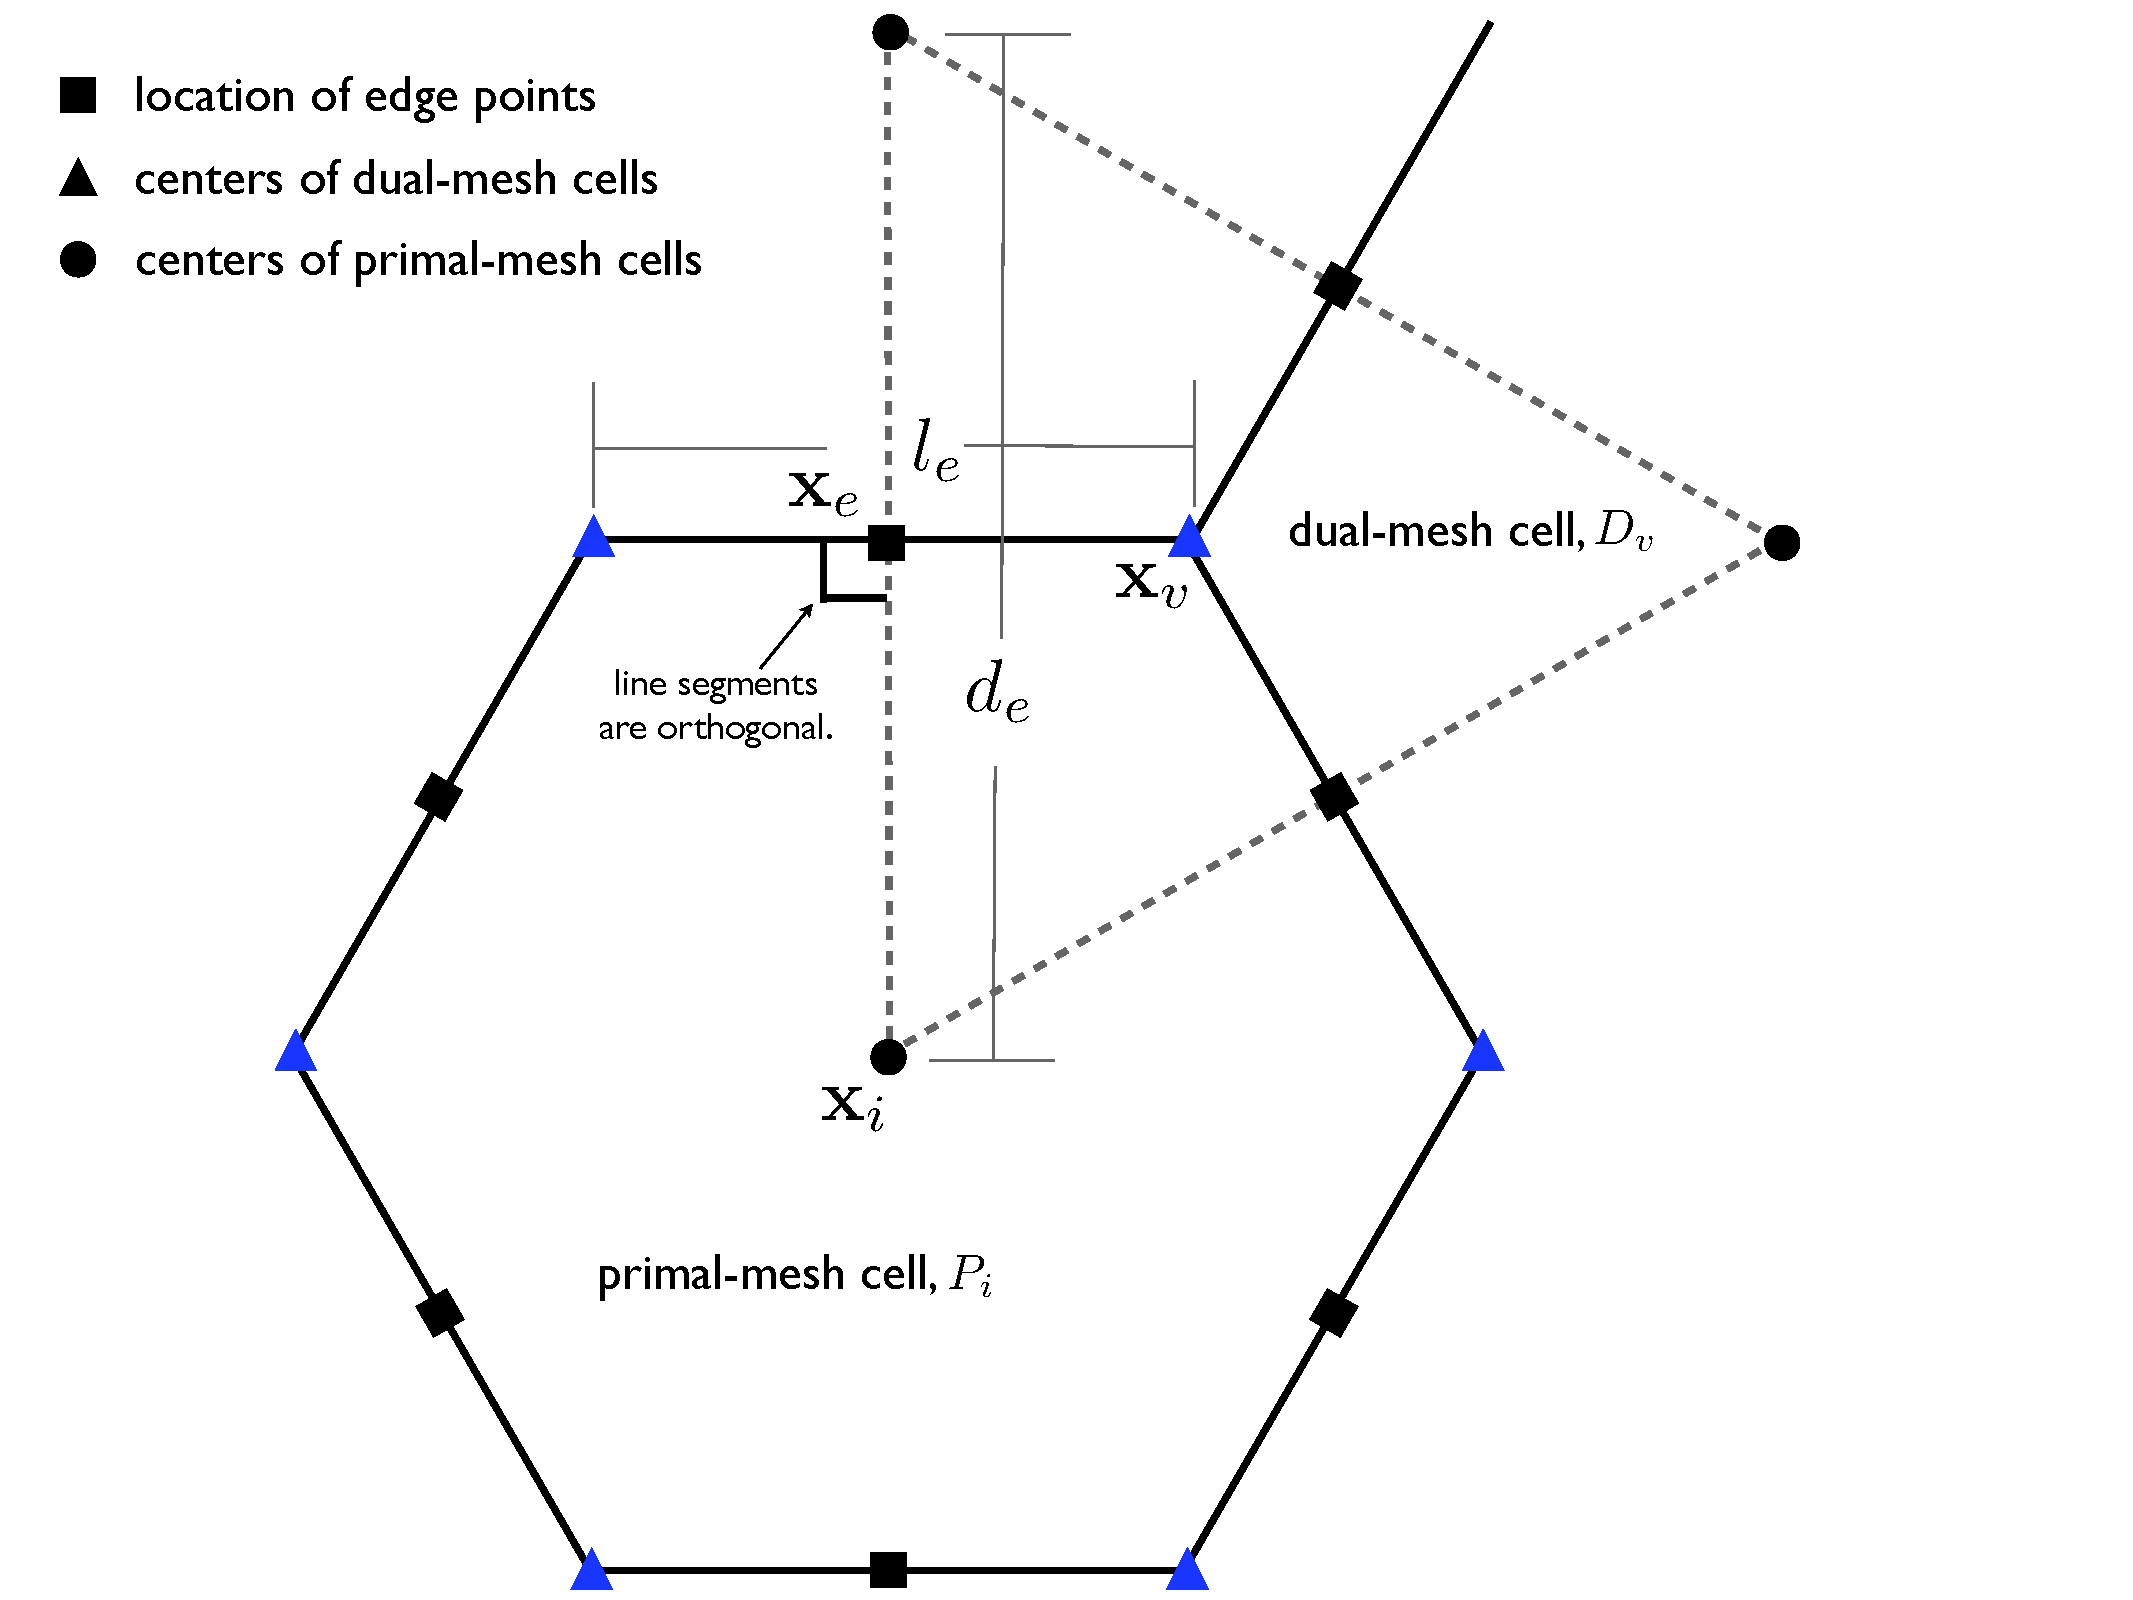
\includegraphics[width=16cm,angle=0]{figures/variablePosition.pdf}\\
  \caption{Definition of elements used to build the MPAS grid. Also see Table \ref{table:variablePosition}.}
  \label{figure:variablePosition}
\end{figure}
%
\begin{table}[p]
\caption{Definition of elements used to build the MPAS grid.}
\label{table:variablePosition}
\begin{center}
\begin{tabular}{lll}
\hline\hline
$Element$ & $Type$ & $Definition$\\
\hline
 ${\bf x}_i$   & point             & location of center of primal-mesh cells \\
 ${\bf x}_v$  &  point            & location of center of dual-mesh cells \\
 ${\bf x}_e$  & point             & location of edge points where velocity is defined \\
 $d_{e}$       & line segment & distance between neighboring ${\bf x}_i$ locations \\
 $l_{e}$       & line segment & distance between neighboring ${\bf x}_v$ locations \\
 $P_i$         & cell                 & a cell on the primal-mesh \\
 $D_v$        & cell                 & a cell on the dual-mesh \\
\hline
\end{tabular}
\end{center}
\end{table}



Table \ref{table:gridFileName} provides the names of all {\it elements} and all {\it sets of elements} as used in the MPAS framework.  Elements appear twice in the table when described in the grid file in more than one way, e.g. points are described with both cartesian and latitude/longitude coordinates. An ``ncdump -h'' of any MPAS grid, output or restart file will contain all variable names shown in second column of Table  \ref{table:gridFileName}.


In addition to these seven element types, we require the definition of {\it sets of elements}. In all, eight different types of sets are required and these are defined and explained in Table \ref{table:gridConnectivity} and Figure \ref{figure:gridConnectivity}. The notation is always of the form of, for example, $i \in CE(e)$, where the LHS indicates the type of element to be gathered (cells) based on the RHS relation to another type of element (edges).

The angle of each edge in an MPAS grid is provided in the variable {\it angleEdge}. The angle
given is the angle between a vector pointing north and a vector pointing in the
positive tangential direction of the edge. Referring to Fig. \ref{fig:angleEdge},
\[ {\rm angleEdge} = \arcsin\|{\bf \hat n} \times {\bf \hat v}\|, \]
where ${\bf \hat n}$ is the unit vector pointing north and ${\bf \hat v}$ is the unit vector
pointing from verticesOnEdge(1,iEdge) to verticesOnEdge(2,iEdge).

Given a wind vector $(u_\perp, u_\parallel)$ defined in term of components orthogonal to
and parallel to the edge, the earth-relative wind $(u,v)$ may be recovered as
\[
\begin{bmatrix}
u \\
v \\
\end{bmatrix}
=
\begin{bmatrix}
\cos\alpha && -\sin\alpha \\
\sin\alpha && \cos\alpha \\
\end{bmatrix}
\begin{bmatrix}
u_\perp \\
u_\parallel \\
\end{bmatrix},
\]
where $\alpha = {\rm angleEdge}$.
\bigskip\bigskip\bigskip


\begin{table}[h]
\caption{Variable names used to describe a MPAS grid.}
\label{table:gridFileName}
\begin{center}
\begin{tabular}{llll}
\hline\hline
$Element$ & $Name$ & $Size$ & $Comment$\\
\hline
 ${\bf x}_i$   & \{x,y,z\}Cell          & nCells  & cartesian location of ${\bf x}_i$  \\
 ${\bf x}_i$   & \{lon,lat\}Cell        & nCells  & longitude and latitude of  ${\bf x}_i$  \\
 ${\bf x}_v$   & \{x,y,z\}Vertex      & nVertices  & cartesian location of ${\bf x}_v$  \\
 ${\bf x}_v$   & \{lon,lat\}Vertex    & nVertices  & longitude and latitude of  ${\bf x}_v$  \\
 ${\bf x}_e$   & \{x,y,z\}Edge          & nEdges  & cartesian location of ${\bf x}_e$  \\
 ${\bf x}_e$   & \{lon,lat\}Edge        & nEdges  & longitude and latitude of  ${\bf x}_e$  \\
 $d_{e}$       & dcEdge                   & nEdges  & distance between ${\bf x}_i$ locations\\
 $l_{e}$         & dvEdge             & nEdges &  distance between ${\bf x}_v$ locations \\
  &  & & \\
 $e \in EC(i) $   &  edgesOnCell  & (nEdgesMax,nCells) & edges that define $P_i$. \\
 $e \in EV(v) $     & edgesOnVertex &  (3,nCells) & edges that define $D_v$. \\
 $i \in CE(e) $      & cellsOnEdge &  (2,nEdges) &  primal-mesh cells that share edge $e$. \\
 $i \in CV(v) $  &   cellsOnVertex &  (3,nVertices) &  primal-mesh cells that define $D_v$. \\
 $v\in VE(e) $  & verticesOnEdge &  (2,nEdges) &    dual-mesh cells that share edge $e$. \\
 $v \in VI(i) $   & verticesOnCell &  (nEdgesMax,nCells) & vertices that define $P_i$. \\
\hline
\end{tabular}
\end{center}
\end{table}
%

%
\begin{table}[p]
\caption{Definition of element groups used to reference connections in the MPAS grid. Examples are provided in Figure \ref{figure:gridConnectivity}.}
\label{table:gridConnectivity}
\begin{center}
\begin{tabular}{lll}
\hline\hline
$Syntax$ & $output$\\
\hline
 $e \in EC(i) $   & set of edges that define the boundary of $P_i$. \\
 $e \in EV(v) $     & set of edges that define the boundary of $D_v$. \\
 $i \in CE(e) $                 & two primal-mesh cells that share edge $e$. \\
 $i \in CV(v) $  &  set of primal-mesh cells that form the vertices of dual mesh cell $D_v$. \\
 $v\in VE(e) $  & the two dual-mesh cells that share edge $e$. \\
 $v \in VI(i) $   & the set of dual-mesh cells that form the vertices of primal-mesh cell $P_i$. \\
 $e \in ECP(e)$ & edges of cell pair meeting at edge $e$. \\
 $e \in EVC(v,i)$ & edge pair associated with vertex $v$ and mesh cell $i$. \\
\hline
\end{tabular}
\end{center}
\end{table}
%
%
\begin{figure}[p]
   \noindent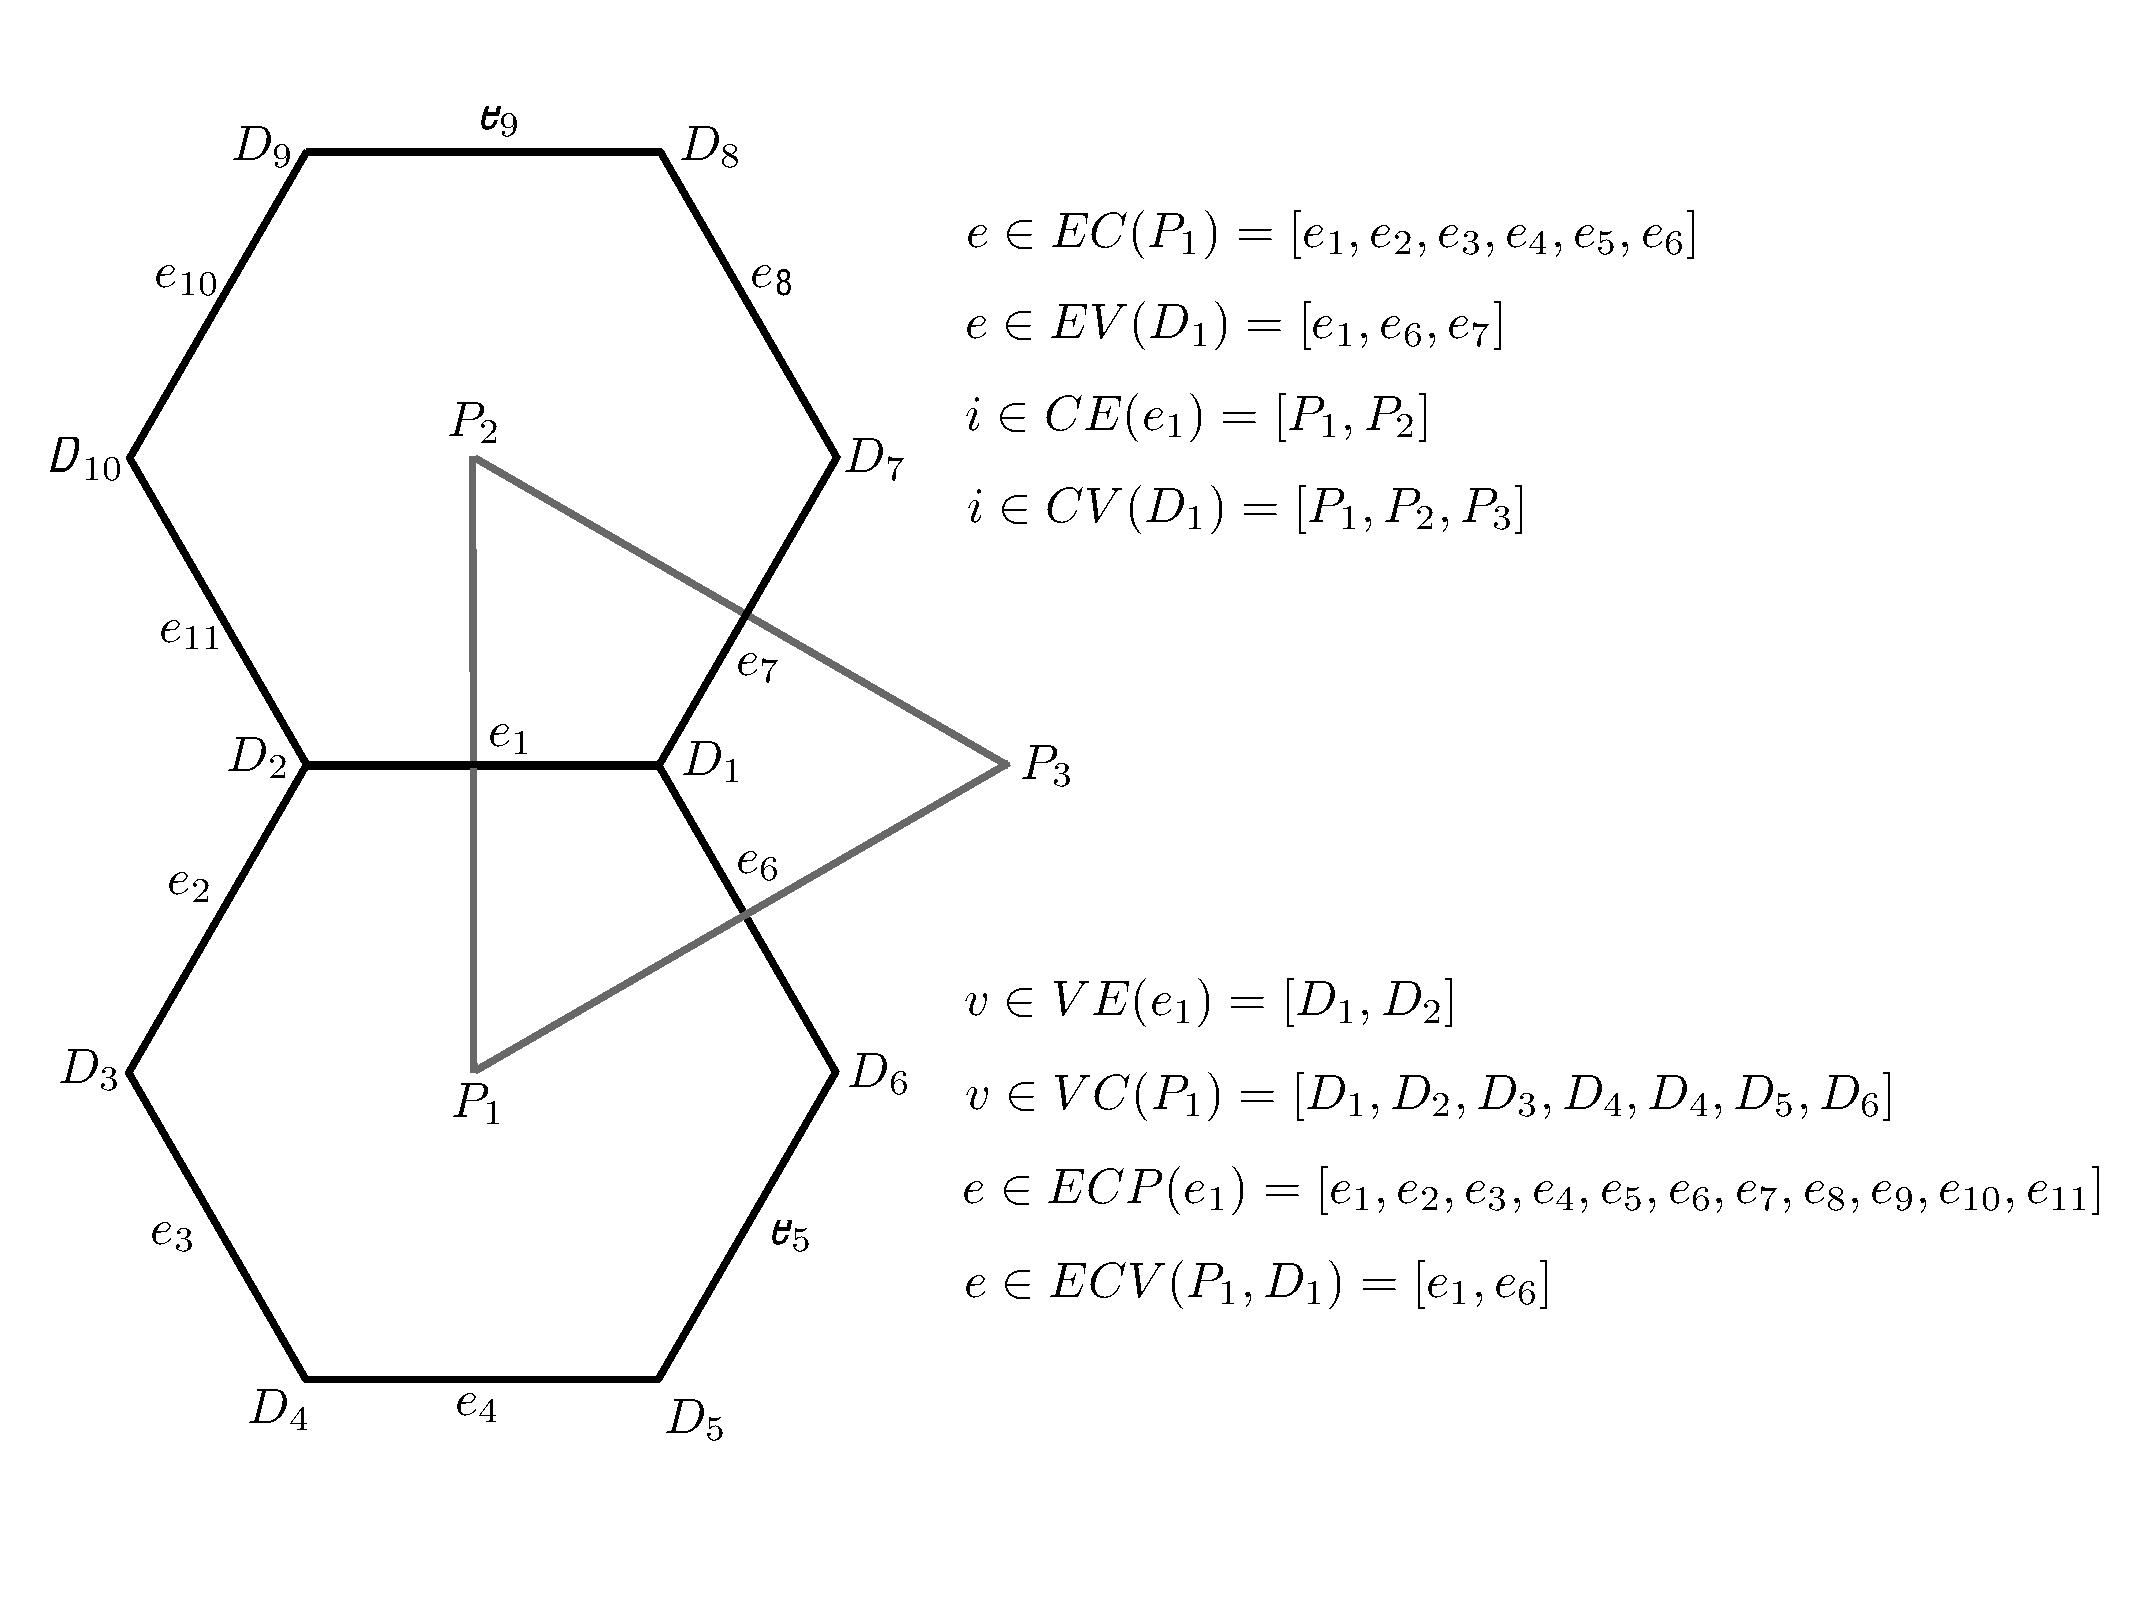
\includegraphics[width=16cm,angle=0]{figures/gridConnectivity.pdf}\\
  \caption{Definition of element groups used to reference connections in the MPAS grid. Also see Table \ref{table:gridConnectivity}.}
  \label{figure:gridConnectivity}
\end{figure}

\begin{figure}[htb]
\begin{center}
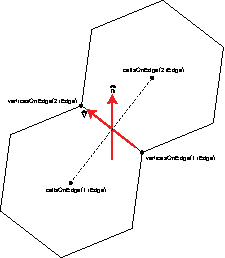
\includegraphics[height=3.2in]{figures/angleEdge.pdf}
\caption{The angle of an edge refers to the angle between a vector pointing north at an edge location
and a vector pointing in the positive tangential velocity direction of the edge.}
\label{fig:angleEdge}
\end{center}
\end{figure}

\vfill \eject

\section{Vertical grid}

The vertical coordinate in MPAS-Atmosphere is $\zeta$ and has units of length, where $0 \le \zeta \le z_{t}$ and  $z_t$ is the height of the model top.  The relationship between the vertical coordinate and height in the physical domain is given as
%
\begin{equation}
z = \zeta + A\, h_s(x,y,\zeta)
\end{equation}
%\label{v_coordinate}
%
where $(x,y)$ denotes a location on the horizontal mesh and $\zeta$ is the vertical coordinate ($\zeta$ is directed radially outward from the surface of the sphere, or perpendicular to the horizontal $(x,y)$ plane in a Cartesian coordinate MPAS-A configuration).  MPAS-A can be configured with the traditional Gal-Chen and Somerville terrain-following coordinate by setting $h_s(x,y,\zeta) = h(x,y)$ and $A = 1-\zeta/z_t$, where $h(x,y)$ is the terrain height.  Alternatively, A can be modified to allow a more rapid or less rapid transition to the constant-height upper boundary condition.  Additionally, a constant-height coordinate can be specified at some intermediate height below $h_t$.

The influence of the terrain on any coordinate surface $\zeta$ can be influenced by the specification of $h_s(x,y,\zeta)$.  Specifically, $h_s$ can be set such that $h_s(x,y,0) = h(x,y)$ (i.e. terrain following at the surface), and progressively filtered fields of $h(x,y)$ can be used at $\zeta > 0$ in $h_s(x,y,\zeta)$, such that the small-scale features in the topography are quickly filtered from the coordinate.  Example MPAS-A vertical meshes are given in Figure \ref{figure:vertical_mesh}

On the MPAS-A mesh C-grid staggering, the state variables $u$, $\rho$, $\theta$ and scalars are located halfway between $w$ levels in both physical height and in the coordinate $\zeta$.  Variables associated with the coordinate systems used in the MPAS-A solver, and possibly appearing in its input, output or history files, are defined in Table \ref{table:vertical_mesh_MPAS-A} and depicted in Figure \ref{figure:vertical_coordinate}.

Further information about the vertical coordinate can be found in \hfil\break
Klemp, J. B. (2011). A Terrain-Following Coordinate with Smoothed Coordinate Surfaces. {\it Mon. Wea. Rev.}, {\bf 139}, 2163-2169. doi:10.1175/MWR-D-10-05046.1

\begin{table}[b]
\caption{Vertical coordinate variables in MPAS-Atmosphere.  $level$ is the integer model level (usually specified with index $k$ where $k=1$ is the lowest model level and physical height increases with increasing k).   $\Delta$ denotes a vertical difference between levels, and $cell$ is a given mesh cell on the primary mesh.}
\label{table:vertical_mesh_MPAS-A}
\begin{center}
\begin{tabular}{lll}
\hline\hline
$Variable$ & $Definition$ \\
\hline
 zgrid($level, cell$)  & physical height of the $w$ points in meters. \\
 zw($level$)     & $\zeta$ at  $w$ levels. \\
 zu($level$)     & $\zeta$ at  $u$ levels; $zu(k) = [zw(k+1)+zw(k)]/2$. \\
 dzw($level$)   & $\Delta \zeta $ at  $u$ levels;  $dzw(k) = zw(k+1)-zw(k)$. \\
 dzu($level$)   & $\Delta \zeta$ at  $w$ levels; $dzu(k) = [dzw(k+1)+dzw(k)]/2$.\\
 rdzw($level$)   & $1/dzw$. \\
 rdzu($level$)   &  $1/dzu$. \\
 zz($level,cell$) & $\Delta \zeta /\Delta z$ at u levels; $(zw(k+1)-zw(k))/(zgrid(k+1,cell)-zgrid(k,cell))$. \\
 fzm($level$)   & weight for linear interpolation to $w(k)$ point for $u(k)$ level variable. \\
 fzp($level$)    & weight for linear interpolation to $w(k)$ point for $u(k-1)$ level variable.  \\
\hline
\end{tabular}
\end{center}
\end{table}



\begin{figure}[t]
\begin{center}
  \noindent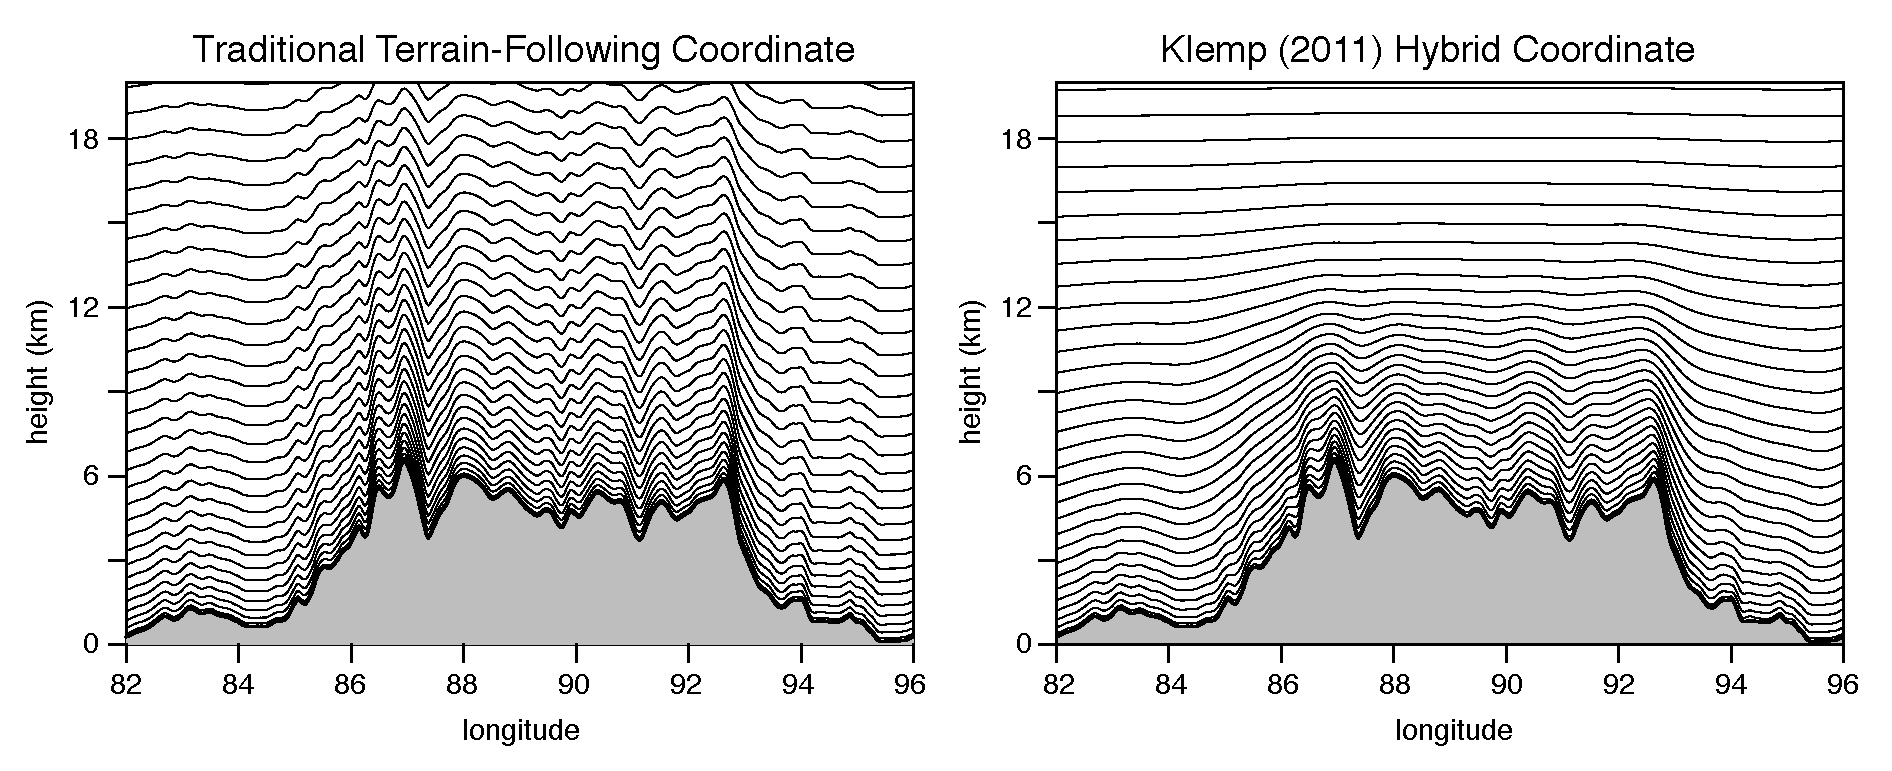
\includegraphics[height=2.6in,angle=0]{figures/MPAS-A_vertical_mesh.pdf}\\
  \caption{Example MPAS-A vertical meshes using terrain following (left) and smoothed (right) vertical coordinates.}
  \label{figure:vertical_mesh}
  \end{center}
\end{figure}

\begin{figure}[t]
\begin{center}
  \noindent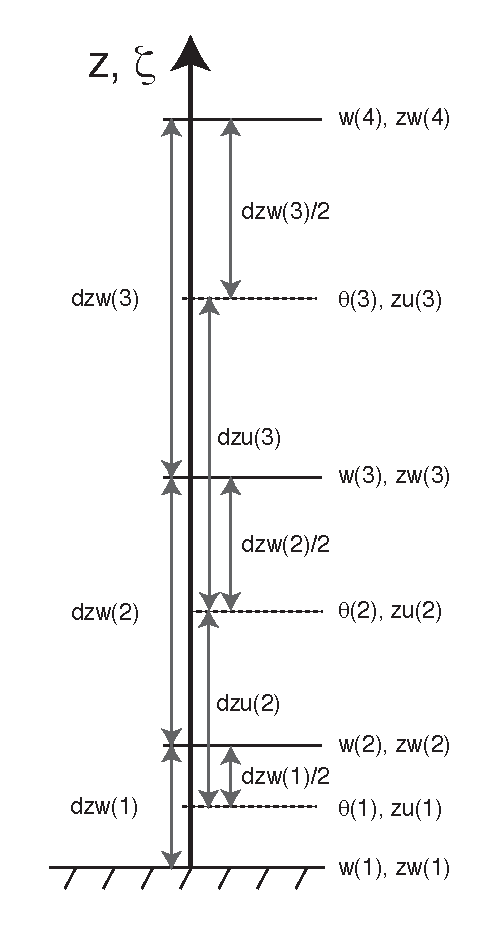
\includegraphics[height=4in,angle=0]{figures/vertical_coordinate_mpas_a.pdf}\\
  \caption{Vertical distribution of the variables in MPAS-A. Also see Table \ref{table:vertical_mesh_MPAS-A}.}
  \label{figure:vertical_coordinate}
  \end{center}
\end{figure}





\chapter{Description of Model Fields}
In this chapter, the fields required in an MPAS input file are described. The dimensionality of each field is given in Fortran storage order (i.e., the fastest-varying dimension is inner-most).
\small

\phantomsection
\addcontentsline{toc}{section}{Fields A--G}

\renewcommand{\arraystretch}{1.5}
\def\bsq#1{\lq{#1}\rq}
\vspace{10mm}
\noindent\begin{minipage}{\textwidth}
\hypertarget{a_tri}
\noindent\textbf{\large{a\_tri}} (real) (nVertLevels, nCells, Time) \\ 
\begin{tabular}{|p{.3\textwidth-2\tabcolsep} |p{.7\textwidth-2\tabcolsep} |} \hline
Units & \textit{unitless} \\ \hline
Description & \textit{implicit tridiagonal solve coefficients} \\ \hline
Accessed in code & as \bsq{a\_tri} from the \bsq{diag} pool \\ \hline
\end{tabular} 
\end{minipage}

\vspace{10mm}
\noindent\begin{minipage}{\textwidth}
\hypertarget{absnxt}
\noindent\textbf{\large{absnxt}} (real) (nVertLevels, cam\_dim1, nCells, Time) \\ 
\begin{tabular}{|p{.3\textwidth-2\tabcolsep} |p{.7\textwidth-2\tabcolsep} |} \hline
Units & \textit{-} \\ \hline
Description & \textit{Total nearest layer absorptivity} \\ \hline
Accessed in code & as \bsq{absnxt} from the \bsq{diag\_physics} pool \\ \hline
\end{tabular} 
\end{minipage}

\vspace{10mm}
\noindent\begin{minipage}{\textwidth}
\hypertarget{abstot}
\noindent\textbf{\large{abstot}} (real) (nVertLevelsP1, nVertLevelsP1, nCells, Time) \\ 
\begin{tabular}{|p{.3\textwidth-2\tabcolsep} |p{.7\textwidth-2\tabcolsep} |} \hline
Units & \textit{-} \\ \hline
Description & \textit{Total absorptivity} \\ \hline
Accessed in code & as \bsq{abstot} from the \bsq{diag\_physics} pool \\ \hline
\end{tabular} 
\end{minipage}

\vspace{10mm}
\noindent\begin{minipage}{\textwidth}
\hypertarget{aclwdnb}
\noindent\textbf{\large{aclwdnb}} (real) (nCells, Time) \\ 
\begin{tabular}{|p{.3\textwidth-2\tabcolsep} |p{.7\textwidth-2\tabcolsep} |} \hline
Units & \textit{W m\textsuperscript{-2}} \\ \hline
Description & \textit{accumulated all-sky downward surface longwave radiation flux} \\ \hline
Accessed in code & as \bsq{aclwdnb} from the \bsq{diag\_physics} pool \\ \hline
\end{tabular} 
\end{minipage}

\vspace{10mm}
\noindent\begin{minipage}{\textwidth}
\hypertarget{aclwdnbc}
\noindent\textbf{\large{aclwdnbc}} (real) (nCells, Time) \\ 
\begin{tabular}{|p{.3\textwidth-2\tabcolsep} |p{.7\textwidth-2\tabcolsep} |} \hline
Units & \textit{W m\textsuperscript{-2}} \\ \hline
Description & \textit{accumulated clear-sky downward surface longwave radiation flux} \\ \hline
Accessed in code & as \bsq{aclwdnbc} from the \bsq{diag\_physics} pool \\ \hline
\end{tabular} 
\end{minipage}

\vspace{10mm}
\noindent\begin{minipage}{\textwidth}
\hypertarget{aclwdnt}
\noindent\textbf{\large{aclwdnt}} (real) (nCells, Time) \\ 
\begin{tabular}{|p{.3\textwidth-2\tabcolsep} |p{.7\textwidth-2\tabcolsep} |} \hline
Units & \textit{W m\textsuperscript{-2}} \\ \hline
Description & \textit{accumulated clear-sky downward surface longwave radiation flux} \\ \hline
Accessed in code & as \bsq{aclwdnt} from the \bsq{diag\_physics} pool \\ \hline
\end{tabular} 
\end{minipage}

\vspace{10mm}
\noindent\begin{minipage}{\textwidth}
\hypertarget{aclwdntc}
\noindent\textbf{\large{aclwdntc}} (real) (nCells, Time) \\ 
\begin{tabular}{|p{.3\textwidth-2\tabcolsep} |p{.7\textwidth-2\tabcolsep} |} \hline
Units & \textit{W m\textsuperscript{-2}} \\ \hline
Description & \textit{accumulated clear-sky downward surface longwave radiation flux} \\ \hline
Accessed in code & as \bsq{aclwdntc} from the \bsq{diag\_physics} pool \\ \hline
\end{tabular} 
\end{minipage}

\vspace{10mm}
\noindent\begin{minipage}{\textwidth}
\hypertarget{aclwupb}
\noindent\textbf{\large{aclwupb}} (real) (nCells, Time) \\ 
\begin{tabular}{|p{.3\textwidth-2\tabcolsep} |p{.7\textwidth-2\tabcolsep} |} \hline
Units & \textit{W m\textsuperscript{-2}} \\ \hline
Description & \textit{accumulated all-sky upward surface longwave radiation flux} \\ \hline
Accessed in code & as \bsq{aclwupb} from the \bsq{diag\_physics} pool \\ \hline
\end{tabular} 
\end{minipage}

\vspace{10mm}
\noindent\begin{minipage}{\textwidth}
\hypertarget{aclwupbc}
\noindent\textbf{\large{aclwupbc}} (real) (nCells, Time) \\ 
\begin{tabular}{|p{.3\textwidth-2\tabcolsep} |p{.7\textwidth-2\tabcolsep} |} \hline
Units & \textit{W m\textsuperscript{-2}} \\ \hline
Description & \textit{accumulated all-sky upward surface longwave radiation flux} \\ \hline
Accessed in code & as \bsq{aclwupbc} from the \bsq{diag\_physics} pool \\ \hline
\end{tabular} 
\end{minipage}

\vspace{10mm}
\noindent\begin{minipage}{\textwidth}
\hypertarget{aclwupt}
\noindent\textbf{\large{aclwupt}} (real) (nCells, Time) \\ 
\begin{tabular}{|p{.3\textwidth-2\tabcolsep} |p{.7\textwidth-2\tabcolsep} |} \hline
Units & \textit{W m\textsuperscript{-2}} \\ \hline
Description & \textit{accumulated all-sky upward surface longwave radiation flux} \\ \hline
Accessed in code & as \bsq{aclwupt} from the \bsq{diag\_physics} pool \\ \hline
\end{tabular} 
\end{minipage}

\vspace{10mm}
\noindent\begin{minipage}{\textwidth}
\hypertarget{aclwuptc}
\noindent\textbf{\large{aclwuptc}} (real) (nCells, Time) \\ 
\begin{tabular}{|p{.3\textwidth-2\tabcolsep} |p{.7\textwidth-2\tabcolsep} |} \hline
Units & \textit{W m\textsuperscript{-2}} \\ \hline
Description & \textit{accumulated all-sky upward surface longwave radiation flux} \\ \hline
Accessed in code & as \bsq{aclwuptc} from the \bsq{diag\_physics} pool \\ \hline
\end{tabular} 
\end{minipage}

\vspace{10mm}
\noindent\begin{minipage}{\textwidth}
\hypertarget{acsnom}
\noindent\textbf{\large{acsnom}} (real) (nCells, Time) \\ 
\begin{tabular}{|p{.3\textwidth-2\tabcolsep} |p{.7\textwidth-2\tabcolsep} |} \hline
Units & \textit{kg m\textsuperscript{-2}} \\ \hline
Description & \textit{accumulated melted snow} \\ \hline
Accessed in code & as \bsq{acsnom} from the \bsq{diag\_physics} pool \\ \hline
\end{tabular} 
\end{minipage}

\vspace{10mm}
\noindent\begin{minipage}{\textwidth}
\hypertarget{acsnow}
\noindent\textbf{\large{acsnow}} (real) (nCells, Time) \\ 
\begin{tabular}{|p{.3\textwidth-2\tabcolsep} |p{.7\textwidth-2\tabcolsep} |} \hline
Units & \textit{kg m\textsuperscript{-2}} \\ \hline
Description & \textit{accumulated snow} \\ \hline
Accessed in code & as \bsq{acsnow} from the \bsq{diag\_physics} pool \\ \hline
\end{tabular} 
\end{minipage}

\vspace{10mm}
\noindent\begin{minipage}{\textwidth}
\hypertarget{acswdnb}
\noindent\textbf{\large{acswdnb}} (real) (nCells, Time) \\ 
\begin{tabular}{|p{.3\textwidth-2\tabcolsep} |p{.7\textwidth-2\tabcolsep} |} \hline
Units & \textit{W m\textsuperscript{-2}} \\ \hline
Description & \textit{accumulated all-sky downward surface shortwave radiation flux} \\ \hline
Accessed in code & as \bsq{acswdnb} from the \bsq{diag\_physics} pool \\ \hline
\end{tabular} 
\end{minipage}

\vspace{10mm}
\noindent\begin{minipage}{\textwidth}
\hypertarget{acswdnbc}
\noindent\textbf{\large{acswdnbc}} (real) (nCells, Time) \\ 
\begin{tabular}{|p{.3\textwidth-2\tabcolsep} |p{.7\textwidth-2\tabcolsep} |} \hline
Units & \textit{W m\textsuperscript{-2}} \\ \hline
Description & \textit{accumulated clear-sky downward surface shortwave radiation flux} \\ \hline
Accessed in code & as \bsq{acswdnbc} from the \bsq{diag\_physics} pool \\ \hline
\end{tabular} 
\end{minipage}

\vspace{10mm}
\noindent\begin{minipage}{\textwidth}
\hypertarget{acswdnt}
\noindent\textbf{\large{acswdnt}} (real) (nCells, Time) \\ 
\begin{tabular}{|p{.3\textwidth-2\tabcolsep} |p{.7\textwidth-2\tabcolsep} |} \hline
Units & \textit{W m\textsuperscript{-2}} \\ \hline
Description & \textit{accumulated all-sky downward top-of-atmosphere shortwave radiation flux} \\ \hline
Accessed in code & as \bsq{acswdnt} from the \bsq{diag\_physics} pool \\ \hline
\end{tabular} 
\end{minipage}

\vspace{10mm}
\noindent\begin{minipage}{\textwidth}
\hypertarget{acswdntc}
\noindent\textbf{\large{acswdntc}} (real) (nCells, Time) \\ 
\begin{tabular}{|p{.3\textwidth-2\tabcolsep} |p{.7\textwidth-2\tabcolsep} |} \hline
Units & \textit{W m\textsuperscript{-2}} \\ \hline
Description & \textit{accumulated clear-sky downward top-of-atmosphere shortwave radiation flux} \\ \hline
Accessed in code & as \bsq{acswdntc} from the \bsq{diag\_physics} pool \\ \hline
\end{tabular} 
\end{minipage}

\vspace{10mm}
\noindent\begin{minipage}{\textwidth}
\hypertarget{acswupb}
\noindent\textbf{\large{acswupb}} (real) (nCells, Time) \\ 
\begin{tabular}{|p{.3\textwidth-2\tabcolsep} |p{.7\textwidth-2\tabcolsep} |} \hline
Units & \textit{W m\textsuperscript{-2}} \\ \hline
Description & \textit{accumulated all-sky upward surface shortwave radiation flux} \\ \hline
Accessed in code & as \bsq{acswupb} from the \bsq{diag\_physics} pool \\ \hline
\end{tabular} 
\end{minipage}

\vspace{10mm}
\noindent\begin{minipage}{\textwidth}
\hypertarget{acswupbc}
\noindent\textbf{\large{acswupbc}} (real) (nCells, Time) \\ 
\begin{tabular}{|p{.3\textwidth-2\tabcolsep} |p{.7\textwidth-2\tabcolsep} |} \hline
Units & \textit{W m\textsuperscript{-2}} \\ \hline
Description & \textit{accumulated clear-sky upward surface shortwave radiation flux} \\ \hline
Accessed in code & as \bsq{acswupbc} from the \bsq{diag\_physics} pool \\ \hline
\end{tabular} 
\end{minipage}

\vspace{10mm}
\noindent\begin{minipage}{\textwidth}
\hypertarget{acswupt}
\noindent\textbf{\large{acswupt}} (real) (nCells, Time) \\ 
\begin{tabular}{|p{.3\textwidth-2\tabcolsep} |p{.7\textwidth-2\tabcolsep} |} \hline
Units & \textit{W m\textsuperscript{-2}} \\ \hline
Description & \textit{accumulated all-sky upward top-of-atmosphere shortwave radiation flux} \\ \hline
Accessed in code & as \bsq{acswupt} from the \bsq{diag\_physics} pool \\ \hline
\end{tabular} 
\end{minipage}

\vspace{10mm}
\noindent\begin{minipage}{\textwidth}
\hypertarget{acswuptc}
\noindent\textbf{\large{acswuptc}} (real) (nCells, Time) \\ 
\begin{tabular}{|p{.3\textwidth-2\tabcolsep} |p{.7\textwidth-2\tabcolsep} |} \hline
Units & \textit{W m\textsuperscript{-2}} \\ \hline
Description & \textit{accumulated clear-sky upward top-of-atmosphere shortwave radiation flux} \\ \hline
Accessed in code & as \bsq{acswuptc} from the \bsq{diag\_physics} pool \\ \hline
\end{tabular} 
\end{minipage}

\vspace{10mm}
\noindent\begin{minipage}{\textwidth}
\hypertarget{aerosols}
\noindent\textbf{\Large{aerosols}} (real) (nAerLevels, nCells, Time) \\ 
\begin{tabular}{|p{.3\textwidth-2\tabcolsep} |p{.7\textwidth-2\tabcolsep} |} \hline
Description & \textit{\bsq{aerosols} is a variable array used in code which is made up of the constituent fields listed below.} \\ \hline
Accessed in code & as \bsq{nr} from the \bsq{state} pool \\ \hline
\end{tabular} 
\end{minipage}

\vspace{5mm}
\noindent Contains constituents:

\vspace{10mm}
\hspace{.1\textwidth}\noindent\begin{minipage}{.9\textwidth}
\hypertarget{sul}
\noindent\textbf{\normalsize{sul}} --- \textit{constituent field of var\_array \textbf{aerosols}}  \\ 
\begin{tabular}{|p{.25\textwidth-.5\tabcolsep} |p{.65\textwidth-1.3\tabcolsep} |} \hline
Description & \textit{Sulfate soluble (SUL) aerosol concentration} \\ \hline
Units & \textit{kg m\textsuperscript{-3}} \\ \hline
Array Group & aer\_cam \\ \hline
\end{tabular} 
\end{minipage}

\vspace{10mm}
\hspace{.1\textwidth}\noindent\begin{minipage}{.9\textwidth}
\hypertarget{sslt}
\noindent\textbf{\normalsize{sslt}} --- \textit{constituent field of var\_array \textbf{aerosols}}  \\ 
\begin{tabular}{|p{.25\textwidth-.5\tabcolsep} |p{.65\textwidth-1.3\tabcolsep} |} \hline
Description & \textit{Sea-salt (SSLT) aerosol concentration} \\ \hline
Units & \textit{kg m\textsuperscript{-3}} \\ \hline
Array Group & aer\_cam \\ \hline
\end{tabular} 
\end{minipage}

\vspace{10mm}
\hspace{.1\textwidth}\noindent\begin{minipage}{.9\textwidth}
\hypertarget{dust1}
\noindent\textbf{\normalsize{dust1}} --- \textit{constituent field of var\_array \textbf{aerosols}}  \\ 
\begin{tabular}{|p{.25\textwidth-.5\tabcolsep} |p{.65\textwidth-1.3\tabcolsep} |} \hline
Description & \textit{Dust type 1 (DUST1) aerosol concentration} \\ \hline
Units & \textit{kg m\textsuperscript{-3}} \\ \hline
Array Group & aer\_cam \\ \hline
\end{tabular} 
\end{minipage}

\vspace{10mm}
\hspace{.1\textwidth}\noindent\begin{minipage}{.9\textwidth}
\hypertarget{dust2}
\noindent\textbf{\normalsize{dust2}} --- \textit{constituent field of var\_array \textbf{aerosols}}  \\ 
\begin{tabular}{|p{.25\textwidth-.5\tabcolsep} |p{.65\textwidth-1.3\tabcolsep} |} \hline
Description & \textit{Dust type 2 (DUST2) aerosol concentration} \\ \hline
Units & \textit{kg m\textsuperscript{-3}} \\ \hline
Array Group & aer\_cam \\ \hline
\end{tabular} 
\end{minipage}

\vspace{10mm}
\hspace{.1\textwidth}\noindent\begin{minipage}{.9\textwidth}
\hypertarget{dust3}
\noindent\textbf{\normalsize{dust3}} --- \textit{constituent field of var\_array \textbf{aerosols}}  \\ 
\begin{tabular}{|p{.25\textwidth-.5\tabcolsep} |p{.65\textwidth-1.3\tabcolsep} |} \hline
Description & \textit{Dust type 3 (DUST3) aerosol concentration} \\ \hline
Units & \textit{kg m\textsuperscript{-3}} \\ \hline
Array Group & aer\_cam \\ \hline
\end{tabular} 
\end{minipage}

\vspace{10mm}
\hspace{.1\textwidth}\noindent\begin{minipage}{.9\textwidth}
\hypertarget{dust4}
\noindent\textbf{\normalsize{dust4}} --- \textit{constituent field of var\_array \textbf{aerosols}}  \\ 
\begin{tabular}{|p{.25\textwidth-.5\tabcolsep} |p{.65\textwidth-1.3\tabcolsep} |} \hline
Description & \textit{Dust type 4 (DUST4) aerosol concentration} \\ \hline
Units & \textit{kg m\textsuperscript{-3}} \\ \hline
Array Group & aer\_cam \\ \hline
\end{tabular} 
\end{minipage}

\vspace{10mm}
\hspace{.1\textwidth}\noindent\begin{minipage}{.9\textwidth}
\hypertarget{ocpho}
\noindent\textbf{\normalsize{ocpho}} --- \textit{constituent field of var\_array \textbf{aerosols}}  \\ 
\begin{tabular}{|p{.25\textwidth-.5\tabcolsep} |p{.65\textwidth-1.3\tabcolsep} |} \hline
Description & \textit{Hydrophobic organic carbon (OCPHO) aerosol concentration} \\ \hline
Units & \textit{kg m\textsuperscript{-3}} \\ \hline
Array Group & aer\_cam \\ \hline
\end{tabular} 
\end{minipage}

\vspace{10mm}
\hspace{.1\textwidth}\noindent\begin{minipage}{.9\textwidth}
\hypertarget{bcpho}
\noindent\textbf{\normalsize{bcpho}} --- \textit{constituent field of var\_array \textbf{aerosols}}  \\ 
\begin{tabular}{|p{.25\textwidth-.5\tabcolsep} |p{.65\textwidth-1.3\tabcolsep} |} \hline
Description & \textit{Hydrophobic black carbon (BCPHO) aerosol concentration} \\ \hline
Units & \textit{kg m\textsuperscript{-3}} \\ \hline
Array Group & aer\_cam \\ \hline
\end{tabular} 
\end{minipage}

\vspace{10mm}
\hspace{.1\textwidth}\noindent\begin{minipage}{.9\textwidth}
\hypertarget{ocphi}
\noindent\textbf{\normalsize{ocphi}} --- \textit{constituent field of var\_array \textbf{aerosols}}  \\ 
\begin{tabular}{|p{.25\textwidth-.5\tabcolsep} |p{.65\textwidth-1.3\tabcolsep} |} \hline
Description & \textit{Hydrophilic organic carbon (OCPHI) aerosol concentration} \\ \hline
Units & \textit{kg m\textsuperscript{-3}} \\ \hline
Array Group & aer\_cam \\ \hline
\end{tabular} 
\end{minipage}

\vspace{10mm}
\hspace{.1\textwidth}\noindent\begin{minipage}{.9\textwidth}
\hypertarget{bcphi}
\noindent\textbf{\normalsize{bcphi}} --- \textit{constituent field of var\_array \textbf{aerosols}}  \\ 
\begin{tabular}{|p{.25\textwidth-.5\tabcolsep} |p{.65\textwidth-1.3\tabcolsep} |} \hline
Description & \textit{Hydrophilic black carbon (BCPHI) aerosol concentration} \\ \hline
Units & \textit{kg m\textsuperscript{-3}} \\ \hline
Array Group & aer\_cam \\ \hline
\end{tabular} 
\end{minipage}

\vspace{10mm}
\hspace{.1\textwidth}\noindent\begin{minipage}{.9\textwidth}
\hypertarget{bg}
\noindent\textbf{\normalsize{bg}} --- \textit{constituent field of var\_array \textbf{aerosols}}  \\ 
\begin{tabular}{|p{.25\textwidth-.5\tabcolsep} |p{.65\textwidth-1.3\tabcolsep} |} \hline
Description & \textit{Background (BG) aerosol concentration} \\ \hline
Units & \textit{kg m\textsuperscript{-3}} \\ \hline
Array Group & aer\_cam \\ \hline
\end{tabular} 
\end{minipage}

\vspace{10mm}
\hspace{.1\textwidth}\noindent\begin{minipage}{.9\textwidth}
\hypertarget{volc}
\noindent\textbf{\normalsize{volc}} --- \textit{constituent field of var\_array \textbf{aerosols}}  \\ 
\begin{tabular}{|p{.25\textwidth-.5\tabcolsep} |p{.65\textwidth-1.3\tabcolsep} |} \hline
Description & \textit{Volcanic (VOLC) aerosol concentration} \\ \hline
Units & \textit{kg m\textsuperscript{-3}} \\ \hline
Array Group & aer\_cam \\ \hline
\end{tabular} 
\end{minipage}

\vspace{10mm}
\noindent\begin{minipage}{\textwidth}
\hypertarget{albedo12m}
\noindent\textbf{\large{albedo12m}} (real) (nMonths, nCells) \\ 
\begin{tabular}{|p{.3\textwidth-2\tabcolsep} |p{.7\textwidth-2\tabcolsep} |} \hline
Units & \textit{unitless} \\ \hline
Description & \textit{monthly-mean climatological aurface albedo} \\ \hline
Accessed in code & as \bsq{albedo12m} from the \bsq{sfc\_input} pool \\ \hline
\end{tabular} 
\end{minipage}

\vspace{10mm}
\noindent\begin{minipage}{\textwidth}
\hypertarget{alpha_tri}
\noindent\textbf{\large{alpha\_tri}} (real) (nVertLevels, nCells, Time) \\ 
\begin{tabular}{|p{.3\textwidth-2\tabcolsep} |p{.7\textwidth-2\tabcolsep} |} \hline
Units & \textit{unitless} \\ \hline
Description & \textit{implicit tridiagonal solve coefficients} \\ \hline
Accessed in code & as \bsq{alpha\_tri} from the \bsq{diag} pool \\ \hline
\end{tabular} 
\end{minipage}

\vspace{10mm}
\noindent\hyperlink{aerosols}{\textbf{\large{bcphi}} --- \textit{see \bsq{aerosols}}}

\vspace{10mm}
\noindent\hyperlink{aerosols}{\textbf{\large{bcpho}} --- \textit{see \bsq{aerosols}}}

\vspace{10mm}
\noindent\hyperlink{aerosols}{\textbf{\large{bg}} --- \textit{see \bsq{aerosols}}}

\vspace{10mm}
\noindent\begin{minipage}{\textwidth}
\hypertarget{br}
\noindent\textbf{\large{br}} (real) (nCells, Time) \\ 
\begin{tabular}{|p{.3\textwidth-2\tabcolsep} |p{.7\textwidth-2\tabcolsep} |} \hline
Units & \textit{unitless} \\ \hline
Description & \textit{Richardson number} \\ \hline
Allocated by & mp\_thompson\_in \\ \hline
Accessed in code & as \bsq{br} from the \bsq{diag\_physics} pool \\ \hline
\end{tabular} 
\end{minipage}

\vspace{10mm}
\noindent\begin{minipage}{\textwidth}
\hypertarget{canwat}
\noindent\textbf{\large{canwat}} (real) (nCells, Time) \\ 
\begin{tabular}{|p{.3\textwidth-2\tabcolsep} |p{.7\textwidth-2\tabcolsep} |} \hline
Units & \textit{kg m\textsuperscript{-2}} \\ \hline
Description & \textit{water in canopy} \\ \hline
Accessed in code & as \bsq{canwat} from the \bsq{diag\_physics} pool \\ \hline
\end{tabular} 
\end{minipage}

\vspace{10mm}
\noindent\begin{minipage}{\textwidth}
\hypertarget{cd}
\noindent\textbf{\large{cd}} (real) (nCells, Time) \\ 
\begin{tabular}{|p{.3\textwidth-2\tabcolsep} |p{.7\textwidth-2\tabcolsep} |} \hline
Units & \textit{unitless} \\ \hline
Description & \textit{drag coefficient at 10-meter} \\ \hline
Allocated by & mp\_thompson\_in \\ \hline
Accessed in code & as \bsq{cd} from the \bsq{diag\_physics} pool \\ \hline
\end{tabular} 
\end{minipage}

\vspace{10mm}
\noindent\begin{minipage}{\textwidth}
\hypertarget{cda}
\noindent\textbf{\large{cda}} (real) (nCells, Time) \\ 
\begin{tabular}{|p{.3\textwidth-2\tabcolsep} |p{.7\textwidth-2\tabcolsep} |} \hline
Units & \textit{unitless} \\ \hline
Description & \textit{drag coefficient at lowest model level} \\ \hline
Allocated by & mp\_thompson\_in \\ \hline
Accessed in code & as \bsq{cda} from the \bsq{diag\_physics} pool \\ \hline
\end{tabular} 
\end{minipage}

\vspace{10mm}
\noindent\begin{minipage}{\textwidth}
\hypertarget{ch}
\noindent\textbf{\large{ch}} (real) (nCells, Time) \\ 
\begin{tabular}{|p{.3\textwidth-2\tabcolsep} |p{.7\textwidth-2\tabcolsep} |} \hline
Units & \textit{m s\textsuperscript{-1}} \\ \hline
Description & \textit{surface exchange coefficient for heat} \\ \hline
Allocated by & mp\_thompson\_in \\ \hline
Accessed in code & as \bsq{ch} from the \bsq{diag\_physics} pool \\ \hline
\end{tabular} 
\end{minipage}

\vspace{10mm}
\noindent\begin{minipage}{\textwidth}
\hypertarget{chklowq}
\noindent\textbf{\large{chklowq}} (real) (nCells, Time) \\ 
\begin{tabular}{|p{.3\textwidth-2\tabcolsep} |p{.7\textwidth-2\tabcolsep} |} \hline
Units & \textit{unitless} \\ \hline
Description & \textit{surface saturation flag} \\ \hline
Accessed in code & as \bsq{chklowq} from the \bsq{diag\_physics} pool \\ \hline
\end{tabular} 
\end{minipage}

\vspace{10mm}
\noindent\begin{minipage}{\textwidth}
\hypertarget{chs}
\noindent\textbf{\large{chs}} (real) (nCells, Time) \\ 
\begin{tabular}{|p{.3\textwidth-2\tabcolsep} |p{.7\textwidth-2\tabcolsep} |} \hline
Units & \textit{m s\textsuperscript{-1}} \\ \hline
Description & \textit{surface exchange coefficient for heat and moisture} \\ \hline
Allocated by & mp\_thompson\_in \\ \hline
Accessed in code & as \bsq{chs} from the \bsq{diag\_physics} pool \\ \hline
\end{tabular} 
\end{minipage}

\vspace{10mm}
\noindent\begin{minipage}{\textwidth}
\hypertarget{chs2}
\noindent\textbf{\large{chs2}} (real) (nCells, Time) \\ 
\begin{tabular}{|p{.3\textwidth-2\tabcolsep} |p{.7\textwidth-2\tabcolsep} |} \hline
Units & \textit{m s\textsuperscript{-1}} \\ \hline
Description & \textit{surface exchange coefficient for heat at 2-meter} \\ \hline
Allocated by & mp\_thompson\_in \\ \hline
Accessed in code & as \bsq{chs2} from the \bsq{diag\_physics} pool \\ \hline
\end{tabular} 
\end{minipage}

\vspace{10mm}
\noindent\begin{minipage}{\textwidth}
\hypertarget{circulation}
\noindent\textbf{\large{circulation}} (real) (nVertLevels, nVertices, Time) \\ 
\begin{tabular}{|p{.3\textwidth-2\tabcolsep} |p{.7\textwidth-2\tabcolsep} |} \hline
Units & \textit{m\textsuperscript2 s\textsuperscript{-1}} \\ \hline
Description & \textit{Horizontal circulation at vertices} \\ \hline
Accessed in code & as \bsq{circulation} from the \bsq{diag} pool \\ \hline
\end{tabular} 
\end{minipage}

\vspace{10mm}
\noindent\begin{minipage}{\textwidth}
\hypertarget{ck}
\noindent\textbf{\large{ck}} (real) (nCells, Time) \\ 
\begin{tabular}{|p{.3\textwidth-2\tabcolsep} |p{.7\textwidth-2\tabcolsep} |} \hline
Units & \textit{unitless} \\ \hline
Description & \textit{enthalpy exchange coeff at 10-meter} \\ \hline
Allocated by & mp\_thompson\_in \\ \hline
Accessed in code & as \bsq{ck} from the \bsq{diag\_physics} pool \\ \hline
\end{tabular} 
\end{minipage}

\vspace{10mm}
\noindent\begin{minipage}{\textwidth}
\hypertarget{cka}
\noindent\textbf{\large{cka}} (real) (nCells, Time) \\ 
\begin{tabular}{|p{.3\textwidth-2\tabcolsep} |p{.7\textwidth-2\tabcolsep} |} \hline
Units & \textit{unitless} \\ \hline
Description & \textit{enthalpy exchange coefficient at lowest model level} \\ \hline
Allocated by & mp\_thompson\_in \\ \hline
Accessed in code & as \bsq{cka} from the \bsq{diag\_physics} pool \\ \hline
\end{tabular} 
\end{minipage}

\vspace{10mm}
\noindent\begin{minipage}{\textwidth}
\hypertarget{cldfrac}
\noindent\textbf{\large{cldfrac}} (real) (nVertLevels, nCells, Time) \\ 
\begin{tabular}{|p{.3\textwidth-2\tabcolsep} |p{.7\textwidth-2\tabcolsep} |} \hline
Units & \textit{unitless} \\ \hline
Description & \textit{horizontal cloud fraction} \\ \hline
Accessed in code & as \bsq{cldfrac} from the \bsq{diag\_physics} pool \\ \hline
\end{tabular} 
\end{minipage}

\vspace{10mm}
\noindent\begin{minipage}{\textwidth}
\hypertarget{cofrz}
\noindent\textbf{\large{cofrz}} (real) (nVertLevels, Time) \\ 
\begin{tabular}{|p{.3\textwidth-2\tabcolsep} |p{.7\textwidth-2\tabcolsep} |} \hline
Units & \textit{s m\textsuperscript{-1}} \\ \hline
Description & \textit{coefficient for implicit contribution of Omega to density update} \\ \hline
Accessed in code & as \bsq{cofrz} from the \bsq{diag} pool \\ \hline
\end{tabular} 
\end{minipage}

\vspace{10mm}
\noindent\begin{minipage}{\textwidth}
\hypertarget{coftz}
\noindent\textbf{\large{coftz}} (real) (nVertLevelsP1, nCells, Time) \\ 
\begin{tabular}{|p{.3\textwidth-2\tabcolsep} |p{.7\textwidth-2\tabcolsep} |} \hline
Units & \textit{s K} \\ \hline
Description & \textit{coefficient for implicit contribution of omega vertical derivative to the theta\_m update} \\ \hline
Accessed in code & as \bsq{coftz} from the \bsq{diag} pool \\ \hline
\end{tabular} 
\end{minipage}

\vspace{10mm}
\noindent\begin{minipage}{\textwidth}
\hypertarget{cofwr}
\noindent\textbf{\large{cofwr}} (real) (nVertLevels, nCells, Time) \\ 
\begin{tabular}{|p{.3\textwidth-2\tabcolsep} |p{.7\textwidth-2\tabcolsep} |} \hline
Units & \textit{m s\textsuperscript{-1}} \\ \hline
Description & \textit{coefficient for implicit contribution of density to the vertical velocity update} \\ \hline
Accessed in code & as \bsq{cofwr} from the \bsq{diag} pool \\ \hline
\end{tabular} 
\end{minipage}

\vspace{10mm}
\noindent\begin{minipage}{\textwidth}
\hypertarget{cofwt}
\noindent\textbf{\large{cofwt}} (real) (nVertLevels, nCells, Time) \\ 
\begin{tabular}{|p{.3\textwidth-2\tabcolsep} |p{.7\textwidth-2\tabcolsep} |} \hline
Units & \textit{m s\textsuperscript{-1} K\textsuperscript{-1}} \\ \hline
Description & \textit{coefficient for implicit contribution of density to the vertical velocity update} \\ \hline
Accessed in code & as \bsq{cofwt} from the \bsq{diag} pool \\ \hline
\end{tabular} 
\end{minipage}

\vspace{10mm}
\noindent\begin{minipage}{\textwidth}
\hypertarget{cofwz}
\noindent\textbf{\large{cofwz}} (real) (nVertLevels, nCells, Time) \\ 
\begin{tabular}{|p{.3\textwidth-2\tabcolsep} |p{.7\textwidth-2\tabcolsep} |} \hline
Units & \textit{m s\textsuperscript{-1} K\textsuperscript{-1}} \\ \hline
Description & \textit{coefficient for implicit contribution of density to the vertical velocity update} \\ \hline
Accessed in code & as \bsq{cofwz} from the \bsq{diag} pool \\ \hline
\end{tabular} 
\end{minipage}

\vspace{10mm}
\noindent\begin{minipage}{\textwidth}
\hypertarget{con}
\noindent\textbf{\large{con}} (real) (nCells) \\ 
\begin{tabular}{|p{.3\textwidth-2\tabcolsep} |p{.7\textwidth-2\tabcolsep} |} \hline
Units & \textit{m\textsuperscript{2}} \\ \hline
Description & \textit{convexity of orography} \\ \hline
Accessed in code & as \bsq{con} from the \bsq{sfc\_input} pool \\ \hline
\end{tabular} 
\end{minipage}

\vspace{10mm}
\noindent\begin{minipage}{\textwidth}
\hypertarget{coszr}
\noindent\textbf{\large{coszr}} (real) (nCells, Time) \\ 
\begin{tabular}{|p{.3\textwidth-2\tabcolsep} |p{.7\textwidth-2\tabcolsep} |} \hline
Units & \textit{unitless} \\ \hline
Description & \textit{cosine of zenith solar angle} \\ \hline
Accessed in code & as \bsq{coszr} from the \bsq{diag\_physics} pool \\ \hline
\end{tabular} 
\end{minipage}

\vspace{10mm}
\noindent\begin{minipage}{\textwidth}
\hypertarget{cov}
\noindent\textbf{\large{cov}} (real) (nVertLevels, nCells, Time) \\ 
\begin{tabular}{|p{.3\textwidth-2\tabcolsep} |p{.7\textwidth-2\tabcolsep} |} \hline
Units & \textit{K kg kg\textsuperscript{-1}} \\ \hline
Description & \textit{liquid water - liquid water potential temperature covariance} \\ \hline
Allocated by & mp\_thompson\_in \\ \hline
Accessed in code & as \bsq{cov} from the \bsq{diag\_physics} pool \\ \hline
\end{tabular} 
\end{minipage}

\vspace{10mm}
\noindent\begin{minipage}{\textwidth}
\hypertarget{cpm}
\noindent\textbf{\large{cpm}} (real) (nCells, Time) \\ 
\begin{tabular}{|p{.3\textwidth-2\tabcolsep} |p{.7\textwidth-2\tabcolsep} |} \hline
Units & \textit{J K\textsuperscript{-1} kg\textsuperscript{-1}} \\ \hline
Description & \textit{specific heat of dry air at constant pressure at lowest model level} \\ \hline
Allocated by & mp\_thompson\_in \\ \hline
Accessed in code & as \bsq{cpm} from the \bsq{diag\_physics} pool \\ \hline
\end{tabular} 
\end{minipage}

\vspace{10mm}
\noindent\begin{minipage}{\textwidth}
\hypertarget{cqs2}
\noindent\textbf{\large{cqs2}} (real) (nCells, Time) \\ 
\begin{tabular}{|p{.3\textwidth-2\tabcolsep} |p{.7\textwidth-2\tabcolsep} |} \hline
Units & \textit{m s\textsuperscript{-1}} \\ \hline
Description & \textit{surface exchange coefficient for moisture at 2-meter} \\ \hline
Allocated by & mp\_thompson\_in \\ \hline
Accessed in code & as \bsq{cqs2} from the \bsq{diag\_physics} pool \\ \hline
\end{tabular} 
\end{minipage}

\vspace{10mm}
\noindent\begin{minipage}{\textwidth}
\hypertarget{cqu}
\noindent\textbf{\large{cqu}} (real) (nVertLevels, nEdges, Time) \\ 
\begin{tabular}{|p{.3\textwidth-2\tabcolsep} |p{.7\textwidth-2\tabcolsep} |} \hline
Units & \textit{unitless} \\ \hline
Description & \textit{rho\_d/rho\_m at cell edge (u points)} \\ \hline
Accessed in code & as \bsq{cqu} from the \bsq{diag} pool \\ \hline
\end{tabular} 
\end{minipage}

\vspace{10mm}
\noindent\begin{minipage}{\textwidth}
\hypertarget{cqw}
\noindent\textbf{\large{cqw}} (real) (nVertLevels, nCells, Time) \\ 
\begin{tabular}{|p{.3\textwidth-2\tabcolsep} |p{.7\textwidth-2\tabcolsep} |} \hline
Units & \textit{unitless} \\ \hline
Description & \textit{rho\_d/rho\_m at w points} \\ \hline
Accessed in code & as \bsq{cqw} from the \bsq{diag} pool \\ \hline
\end{tabular} 
\end{minipage}

\vspace{10mm}
\noindent\begin{minipage}{\textwidth}
\hypertarget{cubot}
\noindent\textbf{\large{cubot}} (real) (nCells, Time) \\ 
\begin{tabular}{|p{.3\textwidth-2\tabcolsep} |p{.7\textwidth-2\tabcolsep} |} \hline
Units & \textit{unitless} \\ \hline
Description & \textit{index of highest level of convection} \\ \hline
Allocated by & mp\_thompson\_in \\ \hline
Accessed in code & as \bsq{cubot} from the \bsq{diag\_physics} pool \\ \hline
\end{tabular} 
\end{minipage}

\vspace{10mm}
\noindent\begin{minipage}{\textwidth}
\hypertarget{cuprec}
\noindent\textbf{\large{cuprec}} (real) (nCells, Time) \\ 
\begin{tabular}{|p{.3\textwidth-2\tabcolsep} |p{.7\textwidth-2\tabcolsep} |} \hline
Units & \textit{mm s\textsuperscript{-1}} \\ \hline
Description & \textit{convective precipitation rate} \\ \hline
Allocated by & mp\_thompson\_in \\ \hline
Accessed in code & as \bsq{cuprec} from the \bsq{diag\_physics} pool \\ \hline
\end{tabular} 
\end{minipage}

\vspace{10mm}
\noindent\begin{minipage}{\textwidth}
\hypertarget{cutop}
\noindent\textbf{\large{cutop}} (real) (nCells, Time) \\ 
\begin{tabular}{|p{.3\textwidth-2\tabcolsep} |p{.7\textwidth-2\tabcolsep} |} \hline
Units & \textit{unitless} \\ \hline
Description & \textit{index of lowest level of convection} \\ \hline
Allocated by & mp\_thompson\_in \\ \hline
Accessed in code & as \bsq{cutop} from the \bsq{diag\_physics} pool \\ \hline
\end{tabular} 
\end{minipage}

\vspace{10mm}
\noindent\begin{minipage}{\textwidth}
\hypertarget{delta}
\noindent\textbf{\large{delta}} (real) (nCells, Time) \\ 
\begin{tabular}{|p{.3\textwidth-2\tabcolsep} |p{.7\textwidth-2\tabcolsep} |} \hline
Units & \textit{m} \\ \hline
Description & \textit{entrainment layer depth from PBL scheme} \\ \hline
Allocated by & mp\_thompson\_in \\ \hline
Accessed in code & as \bsq{delta} from the \bsq{diag\_physics} pool \\ \hline
\end{tabular} 
\end{minipage}

\vspace{10mm}
\noindent\begin{minipage}{\textwidth}
\hypertarget{divergence}
\noindent\textbf{\large{divergence}} (real) (nVertLevels, nCells, Time) \\ 
\begin{tabular}{|p{.3\textwidth-2\tabcolsep} |p{.7\textwidth-2\tabcolsep} |} \hline
Units & \textit{s\textsuperscript{-1}} \\ \hline
Description & \textit{Horizontal velocity divergence at cell center} \\ \hline
Accessed in code & as \bsq{divergence} from the \bsq{diag} pool \\ \hline
\end{tabular} 
\end{minipage}

\vspace{10mm}
\noindent\begin{minipage}{\textwidth}
\hypertarget{divergence_3d}
\noindent\textbf{\large{divergence\_3d}} (real) (nVertLevels, nCells, Time) \\ 
\begin{tabular}{|p{.3\textwidth-2\tabcolsep} |p{.7\textwidth-2\tabcolsep} |} \hline
Units & \textit{kg m\textsuperscript{-3} s\textsuperscript{-1}} \\ \hline
Description & \textit{3D divergence used for acoustic filtering} \\ \hline
Accessed in code & as \bsq{divergence\_3d} from the \bsq{diag} pool \\ \hline
\end{tabular} 
\end{minipage}

\vspace{10mm}
\noindent\begin{minipage}{\textwidth}
\hypertarget{dqke}
\noindent\textbf{\large{dqke}} (real) (nVertLevels, nCells, Time) \\ 
\begin{tabular}{|p{.3\textwidth-2\tabcolsep} |p{.7\textwidth-2\tabcolsep} |} \hline
Units & \textit{m\textsuperscript{2} s\textsuperscript{-2}} \\ \hline
Description & \textit{TKE change} \\ \hline
Allocated by & mp\_thompson\_in \\ \hline
Accessed in code & as \bsq{dqke} from the \bsq{diag\_physics} pool \\ \hline
\end{tabular} 
\end{minipage}

\vspace{10mm}
\noindent\begin{minipage}{\textwidth}
\hypertarget{dtaux3d}
\noindent\textbf{\large{dtaux3d}} (real) (nVertLevels, nCells, Time) \\ 
\begin{tabular}{|p{.3\textwidth-2\tabcolsep} |p{.7\textwidth-2\tabcolsep} |} \hline
Units & \textit{m s\textsuperscript{-1}} \\ \hline
Description & \textit{gravity wave drag over orography u-stress} \\ \hline
Accessed in code & as \bsq{dtaux3d} from the \bsq{diag\_physics} pool \\ \hline
\end{tabular} 
\end{minipage}

\vspace{10mm}
\noindent\begin{minipage}{\textwidth}
\hypertarget{dtauy3d}
\noindent\textbf{\large{dtauy3d}} (real) (nVertLevels, nCells, Time) \\ 
\begin{tabular}{|p{.3\textwidth-2\tabcolsep} |p{.7\textwidth-2\tabcolsep} |} \hline
Units & \textit{m s\textsuperscript{-1}} \\ \hline
Description & \textit{gravity wave drag over orography v-stress} \\ \hline
Accessed in code & as \bsq{dtauy3d} from the \bsq{diag\_physics} pool \\ \hline
\end{tabular} 
\end{minipage}

\vspace{10mm}
\noindent\begin{minipage}{\textwidth}
\hypertarget{dusfcg}
\noindent\textbf{\large{dusfcg}} (real) (nCells, Time) \\ 
\begin{tabular}{|p{.3\textwidth-2\tabcolsep} |p{.7\textwidth-2\tabcolsep} |} \hline
Units & \textit{Pa m s\textsuperscript{-1}} \\ \hline
Description & \textit{vertically-integrated gravity wave drag over orography u-stress} \\ \hline
Accessed in code & as \bsq{dusfcg} from the \bsq{diag\_physics} pool \\ \hline
\end{tabular} 
\end{minipage}

\vspace{10mm}
\noindent\hyperlink{aerosols}{\textbf{\large{dust1}} --- \textit{see \bsq{aerosols}}}

\vspace{10mm}
\noindent\hyperlink{aerosols}{\textbf{\large{dust2}} --- \textit{see \bsq{aerosols}}}

\vspace{10mm}
\noindent\hyperlink{aerosols}{\textbf{\large{dust3}} --- \textit{see \bsq{aerosols}}}

\vspace{10mm}
\noindent\hyperlink{aerosols}{\textbf{\large{dust4}} --- \textit{see \bsq{aerosols}}}

\vspace{10mm}
\noindent\begin{minipage}{\textwidth}
\hypertarget{dvsfcg}
\noindent\textbf{\large{dvsfcg}} (real) (nCells, Time) \\ 
\begin{tabular}{|p{.3\textwidth-2\tabcolsep} |p{.7\textwidth-2\tabcolsep} |} \hline
Units & \textit{Pa m s\textsuperscript{-1}} \\ \hline
Description & \textit{vertically-integrated gravity wave drag over orography v-stress} \\ \hline
Accessed in code & as \bsq{dvsfcg} from the \bsq{diag\_physics} pool \\ \hline
\end{tabular} 
\end{minipage}

\vspace{10mm}
\noindent\begin{minipage}{\textwidth}
\hypertarget{dzs}
\noindent\textbf{\large{dzs}} (real) (nSoilLevels, nCells, Time) \\ 
\begin{tabular}{|p{.3\textwidth-2\tabcolsep} |p{.7\textwidth-2\tabcolsep} |} \hline
Units & \textit{m} \\ \hline
Description & \textit{soil layer thickness} \\ \hline
Accessed in code & as \bsq{dzs} from the \bsq{sfc\_input} pool \\ \hline
\end{tabular} 
\end{minipage}

\vspace{10mm}
\noindent\begin{minipage}{\textwidth}
\hypertarget{el_pbl}
\noindent\textbf{\large{el\_pbl}} (real) (nVertLevels, nCells, Time) \\ 
\begin{tabular}{|p{.3\textwidth-2\tabcolsep} |p{.7\textwidth-2\tabcolsep} |} \hline
Units & \textit{m} \\ \hline
Description & \textit{mixing length from PBL scheme} \\ \hline
Allocated by & mp\_thompson\_in \\ \hline
Accessed in code & as \bsq{el\_pbl} from the \bsq{diag\_physics} pool \\ \hline
\end{tabular} 
\end{minipage}

\vspace{10mm}
\noindent\begin{minipage}{\textwidth}
\hypertarget{emstot}
\noindent\textbf{\large{emstot}} (real) (nVertLevelsP1, nCells, Time) \\ 
\begin{tabular}{|p{.3\textwidth-2\tabcolsep} |p{.7\textwidth-2\tabcolsep} |} \hline
Units & \textit{-} \\ \hline
Description & \textit{Total emissivity} \\ \hline
Accessed in code & as \bsq{emstot} from the \bsq{diag\_physics} pool \\ \hline
\end{tabular} 
\end{minipage}

\vspace{10mm}
\noindent\begin{minipage}{\textwidth}
\hypertarget{euler_tend_theta}
\noindent\textbf{\large{euler\_tend\_theta}} (real) (nVertLevels, nCells, Time) \\ 
\begin{tabular}{|p{.3\textwidth-2\tabcolsep} |p{.7\textwidth-2\tabcolsep} |} \hline
Units & \textit{kg K m\textsuperscript{-3} s\textsuperscript{-1}} \\ \hline
Description & \textit{tendency of coupled potential temperature rho*theta\_m/zz from dynamics and physics that does not change over a Runge-Kutta timestep (it excludes the flux divergence)} \\ \hline
Accessed in code & as \bsq{theta\_euler} from the \bsq{tend} pool \\ \hline
\end{tabular} 
\end{minipage}

\vspace{10mm}
\noindent\begin{minipage}{\textwidth}
\hypertarget{euler_tend_u}
\noindent\textbf{\large{euler\_tend\_u}} (real) (nVertLevels, nEdges, Time) \\ 
\begin{tabular}{|p{.3\textwidth-2\tabcolsep} |p{.7\textwidth-2\tabcolsep} |} \hline
Units & \textit{m s\textsuperscript{-2}} \\ \hline
Description & \textit{Tendency of u from dynamics} \\ \hline
Accessed in code & as \bsq{u\_euler} from the \bsq{tend} pool \\ \hline
\end{tabular} 
\end{minipage}

\vspace{10mm}
\noindent\begin{minipage}{\textwidth}
\hypertarget{euler_tend_w}
\noindent\textbf{\large{euler\_tend\_w}} (real) (nVertLevelsP1, nCells, Time) \\ 
\begin{tabular}{|p{.3\textwidth-2\tabcolsep} |p{.7\textwidth-2\tabcolsep} |} \hline
Units & \textit{m s\textsuperscript{-2}} \\ \hline
Description & \textit{Tendency of w from dynamics} \\ \hline
Accessed in code & as \bsq{w\_euler} from the \bsq{tend} pool \\ \hline
\end{tabular} 
\end{minipage}

\vspace{10mm}
\noindent\begin{minipage}{\textwidth}
\hypertarget{evapprod}
\noindent\textbf{\large{evapprod}} (real) (nVertLevels, nCells, Time) \\ 
\begin{tabular}{|p{.3\textwidth-2\tabcolsep} |p{.7\textwidth-2\tabcolsep} |} \hline
Units & \textit{s\textsuperscript{-1}} \\ \hline
Description & \textit{rain evaporation rate} \\ \hline
Allocated by & mp\_thompson\_in \\ \hline
Accessed in code & as \bsq{evapprod} from the \bsq{diag\_physics} pool \\ \hline
\end{tabular} 
\end{minipage}

\vspace{10mm}
\noindent\begin{minipage}{\textwidth}
\hypertarget{exch_h}
\noindent\textbf{\large{exch\_h}} (real) (nVertLevels, nCells, Time) \\ 
\begin{tabular}{|p{.3\textwidth-2\tabcolsep} |p{.7\textwidth-2\tabcolsep} |} \hline
Units & \textit{m\textsuperscript{2} s\textsuperscript{-1}} \\ \hline
Description & \textit{exchange coefficient} \\ \hline
Allocated by & mp\_thompson\_in \\ \hline
Accessed in code & as \bsq{exch\_h} from the \bsq{diag\_physics} pool \\ \hline
\end{tabular} 
\end{minipage}

\vspace{10mm}
\noindent\begin{minipage}{\textwidth}
\hypertarget{exner}
\noindent\textbf{\large{exner}} (real) (nVertLevels, nCells, Time) \\ 
\begin{tabular}{|p{.3\textwidth-2\tabcolsep} |p{.7\textwidth-2\tabcolsep} |} \hline
Units & \textit{unitless} \\ \hline
Description & \textit{Exner function} \\ \hline
Accessed in code & as \bsq{exner} from the \bsq{diag} pool \\ \hline
\end{tabular} 
\end{minipage}

\vspace{10mm}
\noindent\begin{minipage}{\textwidth}
\hypertarget{exner_base}
\noindent\textbf{\large{exner\_base}} (real) (nVertLevels, nCells, Time) \\ 
\begin{tabular}{|p{.3\textwidth-2\tabcolsep} |p{.7\textwidth-2\tabcolsep} |} \hline
Units & \textit{unitless} \\ \hline
Description & \textit{Base-state Exner function} \\ \hline
Accessed in code & as \bsq{exner\_base} from the \bsq{diag} pool \\ \hline
\end{tabular} 
\end{minipage}

\vspace{10mm}
\noindent\begin{minipage}{\textwidth}
\hypertarget{fh}
\noindent\textbf{\large{fh}} (real) (nCells, Time) \\ 
\begin{tabular}{|p{.3\textwidth-2\tabcolsep} |p{.7\textwidth-2\tabcolsep} |} \hline
Units & \textit{unitless} \\ \hline
Description & \textit{integrated stability function for heat} \\ \hline
Allocated by & mp\_thompson\_in \\ \hline
Accessed in code & as \bsq{fh} from the \bsq{diag\_physics} pool \\ \hline
\end{tabular} 
\end{minipage}

\vspace{10mm}
\noindent\begin{minipage}{\textwidth}
\hypertarget{flhc}
\noindent\textbf{\large{flhc}} (real) (nCells, Time) \\ 
\begin{tabular}{|p{.3\textwidth-2\tabcolsep} |p{.7\textwidth-2\tabcolsep} |} \hline
Units & \textit{W m\textsuperscript{-2} K\textsuperscript{-1}} \\ \hline
Description & \textit{exchange coefficient for heat} \\ \hline
Allocated by & mp\_thompson\_in \\ \hline
Accessed in code & as \bsq{flhc} from the \bsq{diag\_physics} pool \\ \hline
\end{tabular} 
\end{minipage}

\vspace{10mm}
\noindent\begin{minipage}{\textwidth}
\hypertarget{flqc}
\noindent\textbf{\large{flqc}} (real) (nCells, Time) \\ 
\begin{tabular}{|p{.3\textwidth-2\tabcolsep} |p{.7\textwidth-2\tabcolsep} |} \hline
Units & \textit{kg m\textsuperscript{-2} s\textsuperscript{-1}} \\ \hline
Description & \textit{exchange coefficient for moisture} \\ \hline
Allocated by & mp\_thompson\_in \\ \hline
Accessed in code & as \bsq{flqc} from the \bsq{diag\_physics} pool \\ \hline
\end{tabular} 
\end{minipage}

\vspace{10mm}
\noindent\begin{minipage}{\textwidth}
\hypertarget{fm}
\noindent\textbf{\large{fm}} (real) (nCells, Time) \\ 
\begin{tabular}{|p{.3\textwidth-2\tabcolsep} |p{.7\textwidth-2\tabcolsep} |} \hline
Units & \textit{unitless} \\ \hline
Description & \textit{integrated stability function for moisture} \\ \hline
Allocated by & mp\_thompson\_in \\ \hline
Accessed in code & as \bsq{fm} from the \bsq{diag\_physics} pool \\ \hline
\end{tabular} 
\end{minipage}

\vspace{10mm}
\noindent\begin{minipage}{\textwidth}
\hypertarget{gamma_tri}
\noindent\textbf{\large{gamma\_tri}} (real) (nVertLevels, nCells, Time) \\ 
\begin{tabular}{|p{.3\textwidth-2\tabcolsep} |p{.7\textwidth-2\tabcolsep} |} \hline
Units & \textit{unitless} \\ \hline
Description & \textit{implicit tridiagonal solve coefficients} \\ \hline
Accessed in code & as \bsq{gamma\_tri} from the \bsq{diag} pool \\ \hline
\end{tabular} 
\end{minipage}

\vspace{10mm}
\noindent\begin{minipage}{\textwidth}
\hypertarget{glw}
\noindent\textbf{\large{glw}} (real) (nCells, Time) \\ 
\begin{tabular}{|p{.3\textwidth-2\tabcolsep} |p{.7\textwidth-2\tabcolsep} |} \hline
Units & \textit{W m\textsuperscript{-2}} \\ \hline
Description & \textit{all downward surface longwave radiation} \\ \hline
Accessed in code & as \bsq{glw} from the \bsq{diag\_physics} pool \\ \hline
\end{tabular} 
\end{minipage}

\vspace{10mm}
\noindent\begin{minipage}{\textwidth}
\hypertarget{gradPVn}
\noindent\textbf{\large{gradPVn}} (real) (nVertLevels, nEdges, Time) \\ 
\begin{tabular}{|p{.3\textwidth-2\tabcolsep} |p{.7\textwidth-2\tabcolsep} |} \hline
Units & \textit{???} \\ \hline
Description & \textit{Gradient in the normal direction of PV at edge locations} \\ \hline
Accessed in code & as \bsq{gradPVn} from the \bsq{diag} pool \\ \hline
\end{tabular} 
\end{minipage}

\vspace{10mm}
\noindent\begin{minipage}{\textwidth}
\hypertarget{gradPVt}
\noindent\textbf{\large{gradPVt}} (real) (nVertLevels, nEdges, Time) \\ 
\begin{tabular}{|p{.3\textwidth-2\tabcolsep} |p{.7\textwidth-2\tabcolsep} |} \hline
Units & \textit{???} \\ \hline
Description & \textit{Gradient in the tangential direction of PV at edge locations} \\ \hline
Accessed in code & as \bsq{gradPVt} from the \bsq{diag} pool \\ \hline
\end{tabular} 
\end{minipage}

\vspace{10mm}
\noindent\begin{minipage}{\textwidth}
\hypertarget{graupelnc}
\noindent\textbf{\large{graupelnc}} (real) (nCells, Time) \\ 
\begin{tabular}{|p{.3\textwidth-2\tabcolsep} |p{.7\textwidth-2\tabcolsep} |} \hline
Units & \textit{mm} \\ \hline
Description & \textit{accumulated grid-scale precipitation of graupel} \\ \hline
Allocated by & mp\_thompson\_in \\ \hline
Accessed in code & as \bsq{graupelnc} from the \bsq{diag\_physics} pool \\ \hline
\end{tabular} 
\end{minipage}

\vspace{10mm}
\noindent\begin{minipage}{\textwidth}
\hypertarget{graupelncv}
\noindent\textbf{\large{graupelncv}} (real) (nCells, Time) \\ 
\begin{tabular}{|p{.3\textwidth-2\tabcolsep} |p{.7\textwidth-2\tabcolsep} |} \hline
Units & \textit{mm} \\ \hline
Description & \textit{time-step grid-scale precipitation of graupel} \\ \hline
Allocated by & mp\_thompson\_in \\ \hline
Accessed in code & as \bsq{graupelncv} from the \bsq{diag\_physics} pool \\ \hline
\end{tabular} 
\end{minipage}

\vspace{10mm}
\noindent\begin{minipage}{\textwidth}
\hypertarget{grdflx}
\noindent\textbf{\large{grdflx}} (real) (nCells, Time) \\ 
\begin{tabular}{|p{.3\textwidth-2\tabcolsep} |p{.7\textwidth-2\tabcolsep} |} \hline
Units & \textit{W m\textsuperscript{-2}} \\ \hline
Description & \textit{ground heat flux} \\ \hline
Accessed in code & as \bsq{grdflx} from the \bsq{diag\_physics} pool \\ \hline
\end{tabular} 
\end{minipage}

\vspace{10mm}
\noindent\begin{minipage}{\textwidth}
\hypertarget{greenfrac}
\noindent\textbf{\large{greenfrac}} (real) (nMonths, nCells) \\ 
\begin{tabular}{|p{.3\textwidth-2\tabcolsep} |p{.7\textwidth-2\tabcolsep} |} \hline
Units & \textit{unitless} \\ \hline
Description & \textit{monthly-mean climatological greeness fraction} \\ \hline
Accessed in code & as \bsq{greenfrac} from the \bsq{sfc\_input} pool \\ \hline
\end{tabular} 
\end{minipage}

\vspace{10mm}
\noindent\begin{minipage}{\textwidth}
\hypertarget{gsw}
\noindent\textbf{\large{gsw}} (real) (nCells, Time) \\ 
\begin{tabular}{|p{.3\textwidth-2\tabcolsep} |p{.7\textwidth-2\tabcolsep} |} \hline
Units & \textit{W m\textsuperscript{-2}} \\ \hline
Description & \textit{net surface shortwave radiation flux} \\ \hline
Accessed in code & as \bsq{gsw} from the \bsq{diag\_physics} pool \\ \hline
\end{tabular} 
\end{minipage}

\vspace{10mm}
\noindent\begin{minipage}{\textwidth}
\hypertarget{gz1oz0}
\noindent\textbf{\large{gz1oz0}} (real) (nCells, Time) \\ 
\begin{tabular}{|p{.3\textwidth-2\tabcolsep} |p{.7\textwidth-2\tabcolsep} |} \hline
Units & \textit{unitless} \\ \hline
Description & \textit{log(z/z0) where z0 is roughness length} \\ \hline
Allocated by & mp\_thompson\_in \\ \hline
Accessed in code & as \bsq{gz1oz0} from the \bsq{diag\_physics} pool \\ \hline
\end{tabular} 
\end{minipage}

\phantomsection
\addcontentsline{toc}{section}{Fields H--P}

\vspace{10mm}
\noindent\begin{minipage}{\textwidth}
\hypertarget{h_divergence}
\noindent\textbf{\large{h\_divergence}} (real) (nVertLevels, nCells, Time) \\ 
\begin{tabular}{|p{.3\textwidth-2\tabcolsep} |p{.7\textwidth-2\tabcolsep} |} \hline
Units & \textit{???} \\ \hline
Description & \textit{???} \\ \hline
Accessed in code & as \bsq{h\_divergence} from the \bsq{diag} pool \\ \hline
\end{tabular} 
\end{minipage}

\vspace{10mm}
\noindent\begin{minipage}{\textwidth}
\hypertarget{h_oml}
\noindent\textbf{\large{h\_oml}} (real) (nCells, Time) \\ 
\begin{tabular}{|p{.3\textwidth-2\tabcolsep} |p{.7\textwidth-2\tabcolsep} |} \hline
Units & \textit{m} \\ \hline
Description & \textit{ocean mixed layer depth} \\ \hline
Accessed in code & as \bsq{h\_oml} from the \bsq{diag\_physics} pool \\ \hline
\end{tabular} 
\end{minipage}

\vspace{10mm}
\noindent\begin{minipage}{\textwidth}
\hypertarget{h_oml_initial}
\noindent\textbf{\large{h\_oml\_initial}} (real) (nCells, Time) \\ 
\begin{tabular}{|p{.3\textwidth-2\tabcolsep} |p{.7\textwidth-2\tabcolsep} |} \hline
Units & \textit{m} \\ \hline
Description & \textit{ocean mixed layer depth at initial time} \\ \hline
Accessed in code & as \bsq{h\_oml\_initial} from the \bsq{diag\_physics} pool \\ \hline
\end{tabular} 
\end{minipage}

\vspace{10mm}
\noindent\begin{minipage}{\textwidth}
\hypertarget{hfx}
\noindent\textbf{\large{hfx}} (real) (nCells, Time) \\ 
\begin{tabular}{|p{.3\textwidth-2\tabcolsep} |p{.7\textwidth-2\tabcolsep} |} \hline
Units & \textit{W m\textsuperscript{-2}} \\ \hline
Description & \textit{upward heat flux at the surface} \\ \hline
Allocated by & mp\_thompson\_in \\ \hline
Accessed in code & as \bsq{hfx} from the \bsq{diag\_physics} pool \\ \hline
\end{tabular} 
\end{minipage}

\vspace{10mm}
\noindent\begin{minipage}{\textwidth}
\hypertarget{hpbl}
\noindent\textbf{\large{hpbl}} (real) (nCells, Time) \\ 
\begin{tabular}{|p{.3\textwidth-2\tabcolsep} |p{.7\textwidth-2\tabcolsep} |} \hline
Units & \textit{m} \\ \hline
Description & \textit{Planetary Boundary Layer (PBL) height} \\ \hline
Allocated by & mp\_thompson\_in \\ \hline
Accessed in code & as \bsq{hpbl} from the \bsq{diag\_physics} pool \\ \hline
\end{tabular} 
\end{minipage}

\vspace{10mm}
\noindent\begin{minipage}{\textwidth}
\hypertarget{hu_oml}
\noindent\textbf{\large{hu\_oml}} (real) (nCells, Time) \\ 
\begin{tabular}{|p{.3\textwidth-2\tabcolsep} |p{.7\textwidth-2\tabcolsep} |} \hline
Units & \textit{m\textsuperscript2 s\textsuperscript{-1}} \\ \hline
Description & \textit{ocean mixed layer integrated u (zonal velocity)} \\ \hline
Accessed in code & as \bsq{hu\_oml} from the \bsq{diag\_physics} pool \\ \hline
\end{tabular} 
\end{minipage}

\vspace{10mm}
\noindent\begin{minipage}{\textwidth}
\hypertarget{hv_oml}
\noindent\textbf{\large{hv\_oml}} (real) (nCells, Time) \\ 
\begin{tabular}{|p{.3\textwidth-2\tabcolsep} |p{.7\textwidth-2\tabcolsep} |} \hline
Units & \textit{m\textsuperscript2 s\textsuperscript{-1}} \\ \hline
Description & \textit{ocean mixed layer integrated v (meridional velocity)} \\ \hline
Accessed in code & as \bsq{hv\_oml} from the \bsq{diag\_physics} pool \\ \hline
\end{tabular} 
\end{minipage}

\vspace{10mm}
\noindent\begin{minipage}{\textwidth}
\hypertarget{i_aclwdnb}
\noindent\textbf{\large{i\_aclwdnb}} (integer) (nCells, Time) \\ 
\begin{tabular}{|p{.3\textwidth-2\tabcolsep} |p{.7\textwidth-2\tabcolsep} |} \hline
Units & \textit{unitless} \\ \hline
Description & \textit{incidence of accumulated all-sky downward surface longwave radiation greater than config\_bucket\_radt} \\ \hline
Accessed in code & as \bsq{i\_aclwdnb} from the \bsq{diag\_physics} pool \\ \hline
\end{tabular} 
\end{minipage}

\vspace{10mm}
\noindent\begin{minipage}{\textwidth}
\hypertarget{i_aclwdnbc}
\noindent\textbf{\large{i\_aclwdnbc}} (integer) (nCells, Time) \\ 
\begin{tabular}{|p{.3\textwidth-2\tabcolsep} |p{.7\textwidth-2\tabcolsep} |} \hline
Units & \textit{unitless} \\ \hline
Description & \textit{incidence of accumulated clear-sky downward surface longwave radiation greater than config\_bucket\_radt} \\ \hline
Accessed in code & as \bsq{i\_aclwdnbc} from the \bsq{diag\_physics} pool \\ \hline
\end{tabular} 
\end{minipage}

\vspace{10mm}
\noindent\begin{minipage}{\textwidth}
\hypertarget{i_aclwdnt}
\noindent\textbf{\large{i\_aclwdnt}} (integer) (nCells, Time) \\ 
\begin{tabular}{|p{.3\textwidth-2\tabcolsep} |p{.7\textwidth-2\tabcolsep} |} \hline
Units & \textit{unitless} \\ \hline
Description & \textit{incidence of accumulated all-sky downward top-of-atmosphere longwave radiation greater than config\_bucket\_radt} \\ \hline
Accessed in code & as \bsq{i\_aclwdnt} from the \bsq{diag\_physics} pool \\ \hline
\end{tabular} 
\end{minipage}

\vspace{10mm}
\noindent\begin{minipage}{\textwidth}
\hypertarget{i_aclwdntc}
\noindent\textbf{\large{i\_aclwdntc}} (integer) (nCells, Time) \\ 
\begin{tabular}{|p{.3\textwidth-2\tabcolsep} |p{.7\textwidth-2\tabcolsep} |} \hline
Units & \textit{unitless} \\ \hline
Description & \textit{incidence of accumulated clear-sky downward top-of-atmosphere longwave radiation greater than config\_bucket\_radt} \\ \hline
Accessed in code & as \bsq{i\_aclwdntc} from the \bsq{diag\_physics} pool \\ \hline
\end{tabular} 
\end{minipage}

\vspace{10mm}
\noindent\begin{minipage}{\textwidth}
\hypertarget{i_aclwupb}
\noindent\textbf{\large{i\_aclwupb}} (integer) (nCells, Time) \\ 
\begin{tabular}{|p{.3\textwidth-2\tabcolsep} |p{.7\textwidth-2\tabcolsep} |} \hline
Units & \textit{unitless} \\ \hline
Description & \textit{incidence of accumulated all-sky upward surface longwave radiation greater than config\_bucket\_radt} \\ \hline
Accessed in code & as \bsq{i\_aclwupb} from the \bsq{diag\_physics} pool \\ \hline
\end{tabular} 
\end{minipage}

\vspace{10mm}
\noindent\begin{minipage}{\textwidth}
\hypertarget{i_aclwupbc}
\noindent\textbf{\large{i\_aclwupbc}} (integer) (nCells, Time) \\ 
\begin{tabular}{|p{.3\textwidth-2\tabcolsep} |p{.7\textwidth-2\tabcolsep} |} \hline
Units & \textit{unitless} \\ \hline
Description & \textit{incidence of accumulated clear-sky upward surface longwave radiation greater than config\_bucket\_radt} \\ \hline
Accessed in code & as \bsq{i\_aclwupbc} from the \bsq{diag\_physics} pool \\ \hline
\end{tabular} 
\end{minipage}

\vspace{10mm}
\noindent\begin{minipage}{\textwidth}
\hypertarget{i_aclwupt}
\noindent\textbf{\large{i\_aclwupt}} (integer) (nCells, Time) \\ 
\begin{tabular}{|p{.3\textwidth-2\tabcolsep} |p{.7\textwidth-2\tabcolsep} |} \hline
Units & \textit{unitless} \\ \hline
Description & \textit{incidence of accumulated all-sky upward top-of-atmosphere longwave radiation greater than config\_bucket\_radt} \\ \hline
Accessed in code & as \bsq{i\_aclwupt} from the \bsq{diag\_physics} pool \\ \hline
\end{tabular} 
\end{minipage}

\vspace{10mm}
\noindent\begin{minipage}{\textwidth}
\hypertarget{i_aclwuptc}
\noindent\textbf{\large{i\_aclwuptc}} (integer) (nCells, Time) \\ 
\begin{tabular}{|p{.3\textwidth-2\tabcolsep} |p{.7\textwidth-2\tabcolsep} |} \hline
Units & \textit{unitless} \\ \hline
Description & \textit{incidence of accumulated clear-sky upward top-of-atmosphere longwave radiation greater than config\_bucket\_radt} \\ \hline
Accessed in code & as \bsq{i\_aclwuptc} from the \bsq{diag\_physics} pool \\ \hline
\end{tabular} 
\end{minipage}

\vspace{10mm}
\noindent\begin{minipage}{\textwidth}
\hypertarget{i_acswdnb}
\noindent\textbf{\large{i\_acswdnb}} (integer) (nCells, Time) \\ 
\begin{tabular}{|p{.3\textwidth-2\tabcolsep} |p{.7\textwidth-2\tabcolsep} |} \hline
Units & \textit{unitless} \\ \hline
Description & \textit{incidence of accumulated all-sky downward surface shortwave radiation greater than config\_bucket\_radt} \\ \hline
Accessed in code & as \bsq{i\_acswdnb} from the \bsq{diag\_physics} pool \\ \hline
\end{tabular} 
\end{minipage}

\vspace{10mm}
\noindent\begin{minipage}{\textwidth}
\hypertarget{i_acswdnbc}
\noindent\textbf{\large{i\_acswdnbc}} (integer) (nCells, Time) \\ 
\begin{tabular}{|p{.3\textwidth-2\tabcolsep} |p{.7\textwidth-2\tabcolsep} |} \hline
Units & \textit{unitless} \\ \hline
Description & \textit{incidence of accumulated clear-sky downward surface shortwave radiation greater than config\_bucket\_radt} \\ \hline
Accessed in code & as \bsq{i\_acswdnbc} from the \bsq{diag\_physics} pool \\ \hline
\end{tabular} 
\end{minipage}

\vspace{10mm}
\noindent\begin{minipage}{\textwidth}
\hypertarget{i_acswdnt}
\noindent\textbf{\large{i\_acswdnt}} (integer) (nCells, Time) \\ 
\begin{tabular}{|p{.3\textwidth-2\tabcolsep} |p{.7\textwidth-2\tabcolsep} |} \hline
Units & \textit{unitless} \\ \hline
Description & \textit{incidence of accumulated all-sky downward top-of-atmosphere shortwave radiation greater than config\_bucket\_radt} \\ \hline
Accessed in code & as \bsq{i\_acswdnt} from the \bsq{diag\_physics} pool \\ \hline
\end{tabular} 
\end{minipage}

\vspace{10mm}
\noindent\begin{minipage}{\textwidth}
\hypertarget{i_acswdntc}
\noindent\textbf{\large{i\_acswdntc}} (integer) (nCells, Time) \\ 
\begin{tabular}{|p{.3\textwidth-2\tabcolsep} |p{.7\textwidth-2\tabcolsep} |} \hline
Units & \textit{unitless} \\ \hline
Description & \textit{incidence of accumulated clear-sky downward top-of-atmosphere shortwave radiation greater than config\_bucket\_radt} \\ \hline
Accessed in code & as \bsq{i\_acswdntc} from the \bsq{diag\_physics} pool \\ \hline
\end{tabular} 
\end{minipage}

\vspace{10mm}
\noindent\begin{minipage}{\textwidth}
\hypertarget{i_acswupb}
\noindent\textbf{\large{i\_acswupb}} (integer) (nCells, Time) \\ 
\begin{tabular}{|p{.3\textwidth-2\tabcolsep} |p{.7\textwidth-2\tabcolsep} |} \hline
Units & \textit{unitless} \\ \hline
Description & \textit{incidence of accumulated all-sky upward surface shortwave radiation greater than config\_bucket\_radt} \\ \hline
Accessed in code & as \bsq{i\_acswupb} from the \bsq{diag\_physics} pool \\ \hline
\end{tabular} 
\end{minipage}

\vspace{10mm}
\noindent\begin{minipage}{\textwidth}
\hypertarget{i_acswupbc}
\noindent\textbf{\large{i\_acswupbc}} (integer) (nCells, Time) \\ 
\begin{tabular}{|p{.3\textwidth-2\tabcolsep} |p{.7\textwidth-2\tabcolsep} |} \hline
Units & \textit{unitless} \\ \hline
Description & \textit{incidence of accumulated clear-sky upward surface shortwave radiation greater than config\_bucket\_radt} \\ \hline
Accessed in code & as \bsq{i\_acswupbc} from the \bsq{diag\_physics} pool \\ \hline
\end{tabular} 
\end{minipage}

\vspace{10mm}
\noindent\begin{minipage}{\textwidth}
\hypertarget{i_acswupt}
\noindent\textbf{\large{i\_acswupt}} (integer) (nCells, Time) \\ 
\begin{tabular}{|p{.3\textwidth-2\tabcolsep} |p{.7\textwidth-2\tabcolsep} |} \hline
Units & \textit{unitless} \\ \hline
Description & \textit{incidence of accumulated all-sky upward top-of-atmosphere shortwave radiation greater than config\_bucket\_radt} \\ \hline
Accessed in code & as \bsq{i\_acswupt} from the \bsq{diag\_physics} pool \\ \hline
\end{tabular} 
\end{minipage}

\vspace{10mm}
\noindent\begin{minipage}{\textwidth}
\hypertarget{i_acswuptc}
\noindent\textbf{\large{i\_acswuptc}} (integer) (nCells, Time) \\ 
\begin{tabular}{|p{.3\textwidth-2\tabcolsep} |p{.7\textwidth-2\tabcolsep} |} \hline
Units & \textit{unitless} \\ \hline
Description & \textit{incidence of accumulated clear-sky upward top-of-atmosphere shortwave radiation greater than config\_bucket\_radt} \\ \hline
Accessed in code & as \bsq{i\_acswuptc} from the \bsq{diag\_physics} pool \\ \hline
\end{tabular} 
\end{minipage}

\vspace{10mm}
\noindent\begin{minipage}{\textwidth}
\hypertarget{i_rainc}
\noindent\textbf{\large{i\_rainc}} (integer) (nCells, Time) \\ 
\begin{tabular}{|p{.3\textwidth-2\tabcolsep} |p{.7\textwidth-2\tabcolsep} |} \hline
Units & \textit{unitless} \\ \hline
Description & \textit{incidence of accumulated convective precipitation greater than config\_bucket\_rainc} \\ \hline
Allocated by & mp\_thompson\_in \\ \hline
Accessed in code & as \bsq{i\_rainc} from the \bsq{diag\_physics} pool \\ \hline
\end{tabular} 
\end{minipage}

\vspace{10mm}
\noindent\begin{minipage}{\textwidth}
\hypertarget{i_rainnc}
\noindent\textbf{\large{i\_rainnc}} (integer) (nCells, Time) \\ 
\begin{tabular}{|p{.3\textwidth-2\tabcolsep} |p{.7\textwidth-2\tabcolsep} |} \hline
Units & \textit{unitless} \\ \hline
Description & \textit{incidence of accumulated grid-scale precipitation greater than config\_bucket\_rainnc} \\ \hline
Allocated by & mp\_thompson\_in \\ \hline
Accessed in code & as \bsq{i\_rainnc} from the \bsq{diag\_physics} pool \\ \hline
\end{tabular} 
\end{minipage}

\vspace{10mm}
\noindent\begin{minipage}{\textwidth}
\hypertarget{isltyp}
\noindent\textbf{\large{isltyp}} (integer) (nCells) \\ 
\begin{tabular}{|p{.3\textwidth-2\tabcolsep} |p{.7\textwidth-2\tabcolsep} |} \hline
Units & \textit{unitless} \\ \hline
Description & \textit{dominant soil category} \\ \hline
Accessed in code & as \bsq{isltyp} from the \bsq{sfc\_input} pool \\ \hline
\end{tabular} 
\end{minipage}

\vspace{10mm}
\noindent\begin{minipage}{\textwidth}
\hypertarget{ivgtyp}
\noindent\textbf{\large{ivgtyp}} (integer) (nCells) \\ 
\begin{tabular}{|p{.3\textwidth-2\tabcolsep} |p{.7\textwidth-2\tabcolsep} |} \hline
Units & \textit{unitless} \\ \hline
Description & \textit{dominant vegetation category} \\ \hline
Accessed in code & as \bsq{ivgtyp} from the \bsq{sfc\_input} pool \\ \hline
\end{tabular} 
\end{minipage}

\vspace{10mm}
\noindent\begin{minipage}{\textwidth}
\hypertarget{k22_shallow}
\noindent\textbf{\large{k22\_shallow}} (integer) (nCells, Time) \\ 
\begin{tabular}{|p{.3\textwidth-2\tabcolsep} |p{.7\textwidth-2\tabcolsep} |} \hline
Units & \textit{unitless} \\ \hline
Description & \textit{index of convection at k22 level in Grell-Freitas convection scheme} \\ \hline
Allocated by & mp\_thompson\_in \\ \hline
Accessed in code & as \bsq{k22\_shallow} from the \bsq{diag\_physics} pool \\ \hline
\end{tabular} 
\end{minipage}

\vspace{10mm}
\noindent\begin{minipage}{\textwidth}
\hypertarget{kbcon_shallow}
\noindent\textbf{\large{kbcon\_shallow}} (integer) (nCells, Time) \\ 
\begin{tabular}{|p{.3\textwidth-2\tabcolsep} |p{.7\textwidth-2\tabcolsep} |} \hline
Units & \textit{unitless} \\ \hline
Description & \textit{index of lowest level of shallow convection in Grell-Freitas convection scheme} \\ \hline
Allocated by & mp\_thompson\_in \\ \hline
Accessed in code & as \bsq{kbcon\_shallow} from the \bsq{diag\_physics} pool \\ \hline
\end{tabular} 
\end{minipage}

\vspace{10mm}
\noindent\begin{minipage}{\textwidth}
\hypertarget{kdiff}
\noindent\textbf{\large{kdiff}} (real) (nVertLevels, nCells, Time) \\ 
\begin{tabular}{|p{.3\textwidth-2\tabcolsep} |p{.7\textwidth-2\tabcolsep} |} \hline
Units & \textit{m\textsuperscript2 s\textsuperscript{-1}} \\ \hline
Description & \textit{Smagorinsky horizontal eddy viscosity} \\ \hline
Accessed in code & as \bsq{kdiff} from the \bsq{diag} pool \\ \hline
\end{tabular} 
\end{minipage}

\vspace{10mm}
\noindent\begin{minipage}{\textwidth}
\hypertarget{ke}
\noindent\textbf{\large{ke}} (real) (nVertLevels, nCells, Time) \\ 
\begin{tabular}{|p{.3\textwidth-2\tabcolsep} |p{.7\textwidth-2\tabcolsep} |} \hline
Units & \textit{m\textsuperscript2 s\textsuperscript{-2}} \\ \hline
Description & \textit{Kinetic energy at a cell center} \\ \hline
Accessed in code & as \bsq{ke} from the \bsq{diag} pool \\ \hline
\end{tabular} 
\end{minipage}

\vspace{10mm}
\noindent\begin{minipage}{\textwidth}
\hypertarget{kpbl}
\noindent\textbf{\large{kpbl}} (integer) (nCells, Time) \\ 
\begin{tabular}{|p{.3\textwidth-2\tabcolsep} |p{.7\textwidth-2\tabcolsep} |} \hline
Units & \textit{unitless} \\ \hline
Description & \textit{index level of PBL top} \\ \hline
Allocated by & mp\_thompson\_in \\ \hline
Accessed in code & as \bsq{kpbl} from the \bsq{diag\_physics} pool \\ \hline
\end{tabular} 
\end{minipage}

\vspace{10mm}
\noindent\begin{minipage}{\textwidth}
\hypertarget{ktop_deep}
\noindent\textbf{\large{ktop\_deep}} (integer) (nCells, Time) \\ 
\begin{tabular}{|p{.3\textwidth-2\tabcolsep} |p{.7\textwidth-2\tabcolsep} |} \hline
Units & \textit{unitless} \\ \hline
Description & \textit{index of highest level of deep convection in Grell-Freitas convection scheme} \\ \hline
Allocated by & mp\_thompson\_in \\ \hline
Accessed in code & as \bsq{ktop\_deep} from the \bsq{diag\_physics} pool \\ \hline
\end{tabular} 
\end{minipage}

\vspace{10mm}
\noindent\begin{minipage}{\textwidth}
\hypertarget{ktop_shallow}
\noindent\textbf{\large{ktop\_shallow}} (integer) (nCells, Time) \\ 
\begin{tabular}{|p{.3\textwidth-2\tabcolsep} |p{.7\textwidth-2\tabcolsep} |} \hline
Units & \textit{unitless} \\ \hline
Description & \textit{index of highest level of shallow convection in Grell-Freitas convection scheme} \\ \hline
Allocated by & mp\_thompson\_in \\ \hline
Accessed in code & as \bsq{ktop\_shallow} from the \bsq{diag\_physics} pool \\ \hline
\end{tabular} 
\end{minipage}

\vspace{10mm}
\noindent\begin{minipage}{\textwidth}
\hypertarget{kzh}
\noindent\textbf{\large{kzh}} (real) (nVertLevels, nCells, Time) \\ 
\begin{tabular}{|p{.3\textwidth-2\tabcolsep} |p{.7\textwidth-2\tabcolsep} |} \hline
Units & \textit{m\textsuperscript{2} s\textsuperscript{-1}} \\ \hline
Description & \textit{vertical diffusion coefficient of potential temperature} \\ \hline
Allocated by & mp\_thompson\_in \\ \hline
Accessed in code & as \bsq{kzh} from the \bsq{diag\_physics} pool \\ \hline
\end{tabular} 
\end{minipage}

\vspace{10mm}
\noindent\begin{minipage}{\textwidth}
\hypertarget{kzm}
\noindent\textbf{\large{kzm}} (real) (nVertLevels, nCells, Time) \\ 
\begin{tabular}{|p{.3\textwidth-2\tabcolsep} |p{.7\textwidth-2\tabcolsep} |} \hline
Units & \textit{m\textsuperscript{2} s\textsuperscript{-1}} \\ \hline
Description & \textit{vertical diffusion coefficient of mommentum} \\ \hline
Allocated by & mp\_thompson\_in \\ \hline
Accessed in code & as \bsq{kzm} from the \bsq{diag\_physics} pool \\ \hline
\end{tabular} 
\end{minipage}

\vspace{10mm}
\noindent\begin{minipage}{\textwidth}
\hypertarget{kzq}
\noindent\textbf{\large{kzq}} (real) (nVertLevels, nCells, Time) \\ 
\begin{tabular}{|p{.3\textwidth-2\tabcolsep} |p{.7\textwidth-2\tabcolsep} |} \hline
Units & \textit{m\textsuperscript{2} s\textsuperscript{-1}} \\ \hline
Description & \textit{vertical diffusion coefficient of water vapor and cloud condensates} \\ \hline
Allocated by & mp\_thompson\_in \\ \hline
Accessed in code & as \bsq{kzq} from the \bsq{diag\_physics} pool \\ \hline
\end{tabular} 
\end{minipage}

\vspace{10mm}
\noindent\begin{minipage}{\textwidth}
\hypertarget{lai}
\noindent\textbf{\large{lai}} (real) (nCells, Time) \\ 
\begin{tabular}{|p{.3\textwidth-2\tabcolsep} |p{.7\textwidth-2\tabcolsep} |} \hline
Units & \textit{m\textsuperscript{-2} m\textsuperscript{-2}} \\ \hline
Description & \textit{leaf area index} \\ \hline
Accessed in code & as \bsq{lai} from the \bsq{diag\_physics} pool \\ \hline
\end{tabular} 
\end{minipage}

\vspace{10mm}
\noindent\begin{minipage}{\textwidth}
\hypertarget{landmask}
\noindent\textbf{\large{landmask}} (integer) (nCells) \\ 
\begin{tabular}{|p{.3\textwidth-2\tabcolsep} |p{.7\textwidth-2\tabcolsep} |} \hline
Units & \textit{unitless} \\ \hline
Description & \textit{land-ocean mask (1=land ; 0=ocean)} \\ \hline
Accessed in code & as \bsq{landmask} from the \bsq{sfc\_input} pool \\ \hline
\end{tabular} 
\end{minipage}

\vspace{10mm}
\noindent\begin{minipage}{\textwidth}
\hypertarget{lh}
\noindent\textbf{\large{lh}} (real) (nCells, Time) \\ 
\begin{tabular}{|p{.3\textwidth-2\tabcolsep} |p{.7\textwidth-2\tabcolsep} |} \hline
Units & \textit{W m\textsuperscript{-2}} \\ \hline
Description & \textit{latent heat flux at the surface} \\ \hline
Allocated by & mp\_thompson\_in \\ \hline
Accessed in code & as \bsq{lh} from the \bsq{diag\_physics} pool \\ \hline
\end{tabular} 
\end{minipage}

\vspace{10mm}
\noindent\begin{minipage}{\textwidth}
\hypertarget{lwcf}
\noindent\textbf{\large{lwcf}} (real) (nCells, Time) \\ 
\begin{tabular}{|p{.3\textwidth-2\tabcolsep} |p{.7\textwidth-2\tabcolsep} |} \hline
Units & \textit{W m\textsuperscript{-2}} \\ \hline
Description & \textit{top-of-atmosphere cloud longwave radiative forcing} \\ \hline
Accessed in code & as \bsq{lwcf} from the \bsq{diag\_physics} pool \\ \hline
\end{tabular} 
\end{minipage}

\vspace{10mm}
\noindent\begin{minipage}{\textwidth}
\hypertarget{lwdnb}
\noindent\textbf{\large{lwdnb}} (real) (nCells, Time) \\ 
\begin{tabular}{|p{.3\textwidth-2\tabcolsep} |p{.7\textwidth-2\tabcolsep} |} \hline
Units & \textit{W m\textsuperscript{-2}} \\ \hline
Description & \textit{all-sky downward surface longwave radiation flux} \\ \hline
Accessed in code & as \bsq{lwdnb} from the \bsq{diag\_physics} pool \\ \hline
\end{tabular} 
\end{minipage}

\vspace{10mm}
\noindent\begin{minipage}{\textwidth}
\hypertarget{lwdnbc}
\noindent\textbf{\large{lwdnbc}} (real) (nCells, Time) \\ 
\begin{tabular}{|p{.3\textwidth-2\tabcolsep} |p{.7\textwidth-2\tabcolsep} |} \hline
Units & \textit{W m\textsuperscript{-2}} \\ \hline
Description & \textit{clear-sky downward surface longwave radiation flux} \\ \hline
Accessed in code & as \bsq{lwdnbc} from the \bsq{diag\_physics} pool \\ \hline
\end{tabular} 
\end{minipage}

\vspace{10mm}
\noindent\begin{minipage}{\textwidth}
\hypertarget{lwdnt}
\noindent\textbf{\large{lwdnt}} (real) (nCells, Time) \\ 
\begin{tabular}{|p{.3\textwidth-2\tabcolsep} |p{.7\textwidth-2\tabcolsep} |} \hline
Units & \textit{W m\textsuperscript{-2}} \\ \hline
Description & \textit{clear-sky downward surface longwave radiation flux} \\ \hline
Accessed in code & as \bsq{lwdnt} from the \bsq{diag\_physics} pool \\ \hline
\end{tabular} 
\end{minipage}

\vspace{10mm}
\noindent\begin{minipage}{\textwidth}
\hypertarget{lwdntc}
\noindent\textbf{\large{lwdntc}} (real) (nCells, Time) \\ 
\begin{tabular}{|p{.3\textwidth-2\tabcolsep} |p{.7\textwidth-2\tabcolsep} |} \hline
Units & \textit{W m\textsuperscript{-2}} \\ \hline
Description & \textit{clear-sky downward surface longwave radiation flux} \\ \hline
Accessed in code & as \bsq{lwdntc} from the \bsq{diag\_physics} pool \\ \hline
\end{tabular} 
\end{minipage}

\vspace{10mm}
\noindent\begin{minipage}{\textwidth}
\hypertarget{lwupb}
\noindent\textbf{\large{lwupb}} (real) (nCells, Time) \\ 
\begin{tabular}{|p{.3\textwidth-2\tabcolsep} |p{.7\textwidth-2\tabcolsep} |} \hline
Units & \textit{W m\textsuperscript{-2}} \\ \hline
Description & \textit{all-sky upward surface longwave radiation flux} \\ \hline
Accessed in code & as \bsq{lwupb} from the \bsq{diag\_physics} pool \\ \hline
\end{tabular} 
\end{minipage}

\vspace{10mm}
\noindent\begin{minipage}{\textwidth}
\hypertarget{lwupbc}
\noindent\textbf{\large{lwupbc}} (real) (nCells, Time) \\ 
\begin{tabular}{|p{.3\textwidth-2\tabcolsep} |p{.7\textwidth-2\tabcolsep} |} \hline
Units & \textit{W m\textsuperscript{-2}} \\ \hline
Description & \textit{all-sky upward surface longwave radiation flux} \\ \hline
Accessed in code & as \bsq{lwupbc} from the \bsq{diag\_physics} pool \\ \hline
\end{tabular} 
\end{minipage}

\vspace{10mm}
\noindent\begin{minipage}{\textwidth}
\hypertarget{lwupt}
\noindent\textbf{\large{lwupt}} (real) (nCells, Time) \\ 
\begin{tabular}{|p{.3\textwidth-2\tabcolsep} |p{.7\textwidth-2\tabcolsep} |} \hline
Units & \textit{W m\textsuperscript{-2}} \\ \hline
Description & \textit{all-sky upward surface longwave radiation flux} \\ \hline
Accessed in code & as \bsq{lwupt} from the \bsq{diag\_physics} pool \\ \hline
\end{tabular} 
\end{minipage}

\vspace{10mm}
\noindent\begin{minipage}{\textwidth}
\hypertarget{lwuptc}
\noindent\textbf{\large{lwuptc}} (real) (nCells, Time) \\ 
\begin{tabular}{|p{.3\textwidth-2\tabcolsep} |p{.7\textwidth-2\tabcolsep} |} \hline
Units & \textit{W m\textsuperscript{-2}} \\ \hline
Description & \textit{all-sky upward surface longwave radiation flux} \\ \hline
Accessed in code & as \bsq{lwuptc} from the \bsq{diag\_physics} pool \\ \hline
\end{tabular} 
\end{minipage}

\vspace{10mm}
\noindent\begin{minipage}{\textwidth}
\hypertarget{m_ps}
\noindent\textbf{\large{m\_ps}} (real) (nCells, Time) \\ 
\begin{tabular}{|p{.3\textwidth-2\tabcolsep} |p{.7\textwidth-2\tabcolsep} |} \hline
Units & \textit{Pa} \\ \hline
Description & \textit{Surface pressure from match on MPAS grid} \\ \hline
Accessed in code & as \bsq{m\_ps} from the \bsq{state} pool \\ \hline
\end{tabular} 
\end{minipage}

\vspace{10mm}
\noindent\begin{minipage}{\textwidth}
\hypertarget{mavail}
\noindent\textbf{\large{mavail}} (real) (nCells, Time) \\ 
\begin{tabular}{|p{.3\textwidth-2\tabcolsep} |p{.7\textwidth-2\tabcolsep} |} \hline
Units & \textit{unitless} \\ \hline
Description & \textit{surface moisture availability (between 0 and 1)} \\ \hline
Allocated by & mp\_thompson\_in \\ \hline
Accessed in code & as \bsq{mavail} from the \bsq{diag\_physics} pool \\ \hline
\end{tabular} 
\end{minipage}

\vspace{10mm}
\noindent\begin{minipage}{\textwidth}
\hypertarget{mminlu}
\noindent\textbf{\large{mminlu}} (text) () \\ 
\begin{tabular}{|p{.3\textwidth-2\tabcolsep} |p{.7\textwidth-2\tabcolsep} |} \hline
Units & \textit{unitless} \\ \hline
Description & \textit{land use classification} \\ \hline
Accessed in code & as \bsq{mminlu} from the \bsq{sfc\_input} pool \\ \hline
\end{tabular} 
\end{minipage}

\vspace{10mm}
\noindent\begin{minipage}{\textwidth}
\hypertarget{mol}
\noindent\textbf{\large{mol}} (real) (nCells, Time) \\ 
\begin{tabular}{|p{.3\textwidth-2\tabcolsep} |p{.7\textwidth-2\tabcolsep} |} \hline
Units & \textit{K} \\ \hline
Description & \textit{T* in similarity theory} \\ \hline
Allocated by & mp\_thompson\_in \\ \hline
Accessed in code & as \bsq{mol} from the \bsq{diag\_physics} pool \\ \hline
\end{tabular} 
\end{minipage}

\vspace{10mm}
\noindent\begin{minipage}{\textwidth}
\hypertarget{mu_c}
\noindent\textbf{\large{mu\_c}} (real) (nCells) \\ 
\begin{tabular}{|p{.3\textwidth-2\tabcolsep} |p{.7\textwidth-2\tabcolsep} |} \hline
Units & \textit{unitless} \\ \hline
Description & \textit{gamma shape parameter} \\ \hline
Allocated by & mp\_thompson\_in \\ \hline
Accessed in code & as \bsq{mu\_c} from the \bsq{diag\_physics} pool \\ \hline
\end{tabular} 
\end{minipage}

\vspace{10mm}
\noindent\begin{minipage}{\textwidth}
\hypertarget{nca}
\noindent\textbf{\large{nca}} (real) (nCells, Time) \\ 
\begin{tabular}{|p{.3\textwidth-2\tabcolsep} |p{.7\textwidth-2\tabcolsep} |} \hline
Units & \textit{s} \\ \hline
Description & \textit{relaxation time for KF parameterization of convection} \\ \hline
Allocated by & mp\_thompson\_in \\ \hline
Accessed in code & as \bsq{nca} from the \bsq{diag\_physics} pool \\ \hline
\end{tabular} 
\end{minipage}

\vspace{10mm}
\noindent\begin{minipage}{\textwidth}
\hypertarget{ndays_accum}
\noindent\textbf{\large{ndays\_accum}} (real) (nCells, Time) \\ 
\begin{tabular}{|p{.3\textwidth-2\tabcolsep} |p{.7\textwidth-2\tabcolsep} |} \hline
Units & \textit{unitless} \\ \hline
Description & \textit{number of accumulated days in a year} \\ \hline
Accessed in code & as \bsq{ndays\_accum} from the \bsq{diag\_physics} pool \\ \hline
\end{tabular} 
\end{minipage}

\vspace{10mm}
\noindent\hyperlink{scalars}{\textbf{\large{ni}} --- \textit{see \bsq{scalars}}}

\vspace{10mm}
\noindent\begin{minipage}{\textwidth}
\hypertarget{nlrad}
\noindent\textbf{\large{nlrad}} (integer) (nCells, Time) \\ 
\begin{tabular}{|p{.3\textwidth-2\tabcolsep} |p{.7\textwidth-2\tabcolsep} |} \hline
Units & \textit{-} \\ \hline
Description & \textit{number of layers added above the model-top in the RRTMG lw radiation code} \\ \hline
Accessed in code & as \bsq{nlrad} from the \bsq{diag\_physics} pool \\ \hline
\end{tabular} 
\end{minipage}

\vspace{10mm}
\noindent\begin{minipage}{\textwidth}
\hypertarget{noahres}
\noindent\textbf{\large{noahres}} (real) (nCells, Time) \\ 
\begin{tabular}{|p{.3\textwidth-2\tabcolsep} |p{.7\textwidth-2\tabcolsep} |} \hline
Units & \textit{W m\textsuperscript{-2}} \\ \hline
Description & \textit{residual of the Noah surface energy budget} \\ \hline
Accessed in code & as \bsq{noahres} from the \bsq{diag\_physics} pool \\ \hline
\end{tabular} 
\end{minipage}

\vspace{10mm}
\noindent\hyperlink{scalars}{\textbf{\large{nr}} --- \textit{see \bsq{scalars}}}

\vspace{10mm}
\noindent\begin{minipage}{\textwidth}
\hypertarget{nsteps_accum}
\noindent\textbf{\large{nsteps\_accum}} (real) (nCells, Time) \\ 
\begin{tabular}{|p{.3\textwidth-2\tabcolsep} |p{.7\textwidth-2\tabcolsep} |} \hline
Units & \textit{unitless} \\ \hline
Description & \textit{number of accumulated time-steps in a day} \\ \hline
Accessed in code & as \bsq{nsteps\_accum} from the \bsq{diag\_physics} pool \\ \hline
\end{tabular} 
\end{minipage}

\vspace{10mm}
\noindent\begin{minipage}{\textwidth}
\hypertarget{nt_c}
\noindent\textbf{\large{nt\_c}} (real) (nCells) \\ 
\begin{tabular}{|p{.3\textwidth-2\tabcolsep} |p{.7\textwidth-2\tabcolsep} |} \hline
Units & \textit{nb kg\textsuperscript{-1}} \\ \hline
Description & \textit{one-moment constant cloud water droplet concentration} \\ \hline
Allocated by & mp\_thompson\_in \\ \hline
Accessed in code & as \bsq{nt\_c} from the \bsq{diag\_physics} pool \\ \hline
\end{tabular} 
\end{minipage}

\vspace{10mm}
\noindent\begin{minipage}{\textwidth}
\hypertarget{o3clim}
\noindent\textbf{\large{o3clim}} (real) (nOznLevels, nCells, Time) \\ 
\begin{tabular}{|p{.3\textwidth-2\tabcolsep} |p{.7\textwidth-2\tabcolsep} |} \hline
Units & \textit{mol mol\textsuperscript{-1}} \\ \hline
Description & \textit{climatological ozone on prescribed pressure levels at current time} \\ \hline
Accessed in code & as \bsq{o3clim} from the \bsq{diag\_physics} pool \\ \hline
\end{tabular} 
\end{minipage}

\vspace{10mm}
\noindent\begin{minipage}{\textwidth}
\hypertarget{o3vmr}
\noindent\textbf{\large{o3vmr}} (real) (nVertLevels, nCells, Time) \\ 
\begin{tabular}{|p{.3\textwidth-2\tabcolsep} |p{.7\textwidth-2\tabcolsep} |} \hline
Units & \textit{mol mol\textsuperscript{-1}} \\ \hline
Description & \textit{ozone volume mixing ratio} \\ \hline
Accessed in code & as \bsq{o3vmr} from the \bsq{diag\_physics} pool \\ \hline
\end{tabular} 
\end{minipage}

\vspace{10mm}
\noindent\begin{minipage}{\textwidth}
\hypertarget{oa1}
\noindent\textbf{\large{oa1}} (real) (nCells) \\ 
\begin{tabular}{|p{.3\textwidth-2\tabcolsep} |p{.7\textwidth-2\tabcolsep} |} \hline
Units & \textit{unitless} \\ \hline
Description & \textit{directional asymmetry function of orography} \\ \hline
Accessed in code & as \bsq{oa1} from the \bsq{sfc\_input} pool \\ \hline
\end{tabular} 
\end{minipage}

\vspace{10mm}
\noindent\begin{minipage}{\textwidth}
\hypertarget{oa2}
\noindent\textbf{\large{oa2}} (real) (nCells) \\ 
\begin{tabular}{|p{.3\textwidth-2\tabcolsep} |p{.7\textwidth-2\tabcolsep} |} \hline
Units & \textit{unitless} \\ \hline
Description & \textit{directional asymmetry function of orography} \\ \hline
Accessed in code & as \bsq{oa2} from the \bsq{sfc\_input} pool \\ \hline
\end{tabular} 
\end{minipage}

\vspace{10mm}
\noindent\begin{minipage}{\textwidth}
\hypertarget{oa3}
\noindent\textbf{\large{oa3}} (real) (nCells) \\ 
\begin{tabular}{|p{.3\textwidth-2\tabcolsep} |p{.7\textwidth-2\tabcolsep} |} \hline
Units & \textit{unitless} \\ \hline
Description & \textit{directional asymmetry function of orography} \\ \hline
Accessed in code & as \bsq{oa3} from the \bsq{sfc\_input} pool \\ \hline
\end{tabular} 
\end{minipage}

\vspace{10mm}
\noindent\begin{minipage}{\textwidth}
\hypertarget{oa4}
\noindent\textbf{\large{oa4}} (real) (nCells) \\ 
\begin{tabular}{|p{.3\textwidth-2\tabcolsep} |p{.7\textwidth-2\tabcolsep} |} \hline
Units & \textit{unitless} \\ \hline
Description & \textit{directional asymmetry function of orography} \\ \hline
Accessed in code & as \bsq{oa4} from the \bsq{sfc\_input} pool \\ \hline
\end{tabular} 
\end{minipage}

\vspace{10mm}
\noindent\hyperlink{aerosols}{\textbf{\large{ocphi}} --- \textit{see \bsq{aerosols}}}

\vspace{10mm}
\noindent\hyperlink{aerosols}{\textbf{\large{ocpho}} --- \textit{see \bsq{aerosols}}}

\vspace{10mm}
\noindent\begin{minipage}{\textwidth}
\hypertarget{ol1}
\noindent\textbf{\large{ol1}} (real) (nCells) \\ 
\begin{tabular}{|p{.3\textwidth-2\tabcolsep} |p{.7\textwidth-2\tabcolsep} |} \hline
Units & \textit{unitless} \\ \hline
Description & \textit{directional asymmetry function of orography} \\ \hline
Accessed in code & as \bsq{ol1} from the \bsq{sfc\_input} pool \\ \hline
\end{tabular} 
\end{minipage}

\vspace{10mm}
\noindent\begin{minipage}{\textwidth}
\hypertarget{ol2}
\noindent\textbf{\large{ol2}} (real) (nCells) \\ 
\begin{tabular}{|p{.3\textwidth-2\tabcolsep} |p{.7\textwidth-2\tabcolsep} |} \hline
Units & \textit{unitless} \\ \hline
Description & \textit{directional asymmetry function of orography} \\ \hline
Accessed in code & as \bsq{ol2} from the \bsq{sfc\_input} pool \\ \hline
\end{tabular} 
\end{minipage}

\vspace{10mm}
\noindent\begin{minipage}{\textwidth}
\hypertarget{ol3}
\noindent\textbf{\large{ol3}} (real) (nCells) \\ 
\begin{tabular}{|p{.3\textwidth-2\tabcolsep} |p{.7\textwidth-2\tabcolsep} |} \hline
Units & \textit{unitles} \\ \hline
Description & \textit{directional asymmetry function of orography} \\ \hline
Accessed in code & as \bsq{ol3} from the \bsq{sfc\_input} pool \\ \hline
\end{tabular} 
\end{minipage}

\vspace{10mm}
\noindent\begin{minipage}{\textwidth}
\hypertarget{ol4}
\noindent\textbf{\large{ol4}} (real) (nCells) \\ 
\begin{tabular}{|p{.3\textwidth-2\tabcolsep} |p{.7\textwidth-2\tabcolsep} |} \hline
Units & \textit{unitless} \\ \hline
Description & \textit{directional asymmetry function of orography} \\ \hline
Accessed in code & as \bsq{ol4} from the \bsq{sfc\_input} pool \\ \hline
\end{tabular} 
\end{minipage}

\vspace{10mm}
\noindent\begin{minipage}{\textwidth}
\hypertarget{olrtoa}
\noindent\textbf{\large{olrtoa}} (real) (nCells, Time) \\ 
\begin{tabular}{|p{.3\textwidth-2\tabcolsep} |p{.7\textwidth-2\tabcolsep} |} \hline
Units & \textit{W m\textsuperscript{-2}} \\ \hline
Description & \textit{top-of-atmosphere outgoing longwave radiation flux} \\ \hline
Accessed in code & as \bsq{olrtoa} from the \bsq{diag\_physics} pool \\ \hline
\end{tabular} 
\end{minipage}

\vspace{10mm}
\noindent\begin{minipage}{\textwidth}
\hypertarget{ozmixm}
\noindent\textbf{\large{ozmixm}} (real) (nMonths, nOznLevels, nCells) \\ 
\begin{tabular}{|p{.3\textwidth-2\tabcolsep} |p{.7\textwidth-2\tabcolsep} |} \hline
Units & \textit{mol mol\textsuperscript{-1}} \\ \hline
Description & \textit{monthly-mean climatological ozone defined at fixed pressure levels} \\ \hline
Accessed in code & as \bsq{ozmixm} from the \bsq{atm\_input} pool \\ \hline
\end{tabular} 
\end{minipage}

\vspace{10mm}
\noindent\begin{minipage}{\textwidth}
\hypertarget{pin}
\noindent\textbf{\large{pin}} (real) (nOznLevels) \\ 
\begin{tabular}{|p{.3\textwidth-2\tabcolsep} |p{.7\textwidth-2\tabcolsep} |} \hline
Units & \textit{Pa} \\ \hline
Description & \textit{fixed pressure levels at which climatological ozone is defined} \\ \hline
Accessed in code & as \bsq{pin} from the \bsq{atm\_input} pool \\ \hline
\end{tabular} 
\end{minipage}

\vspace{10mm}
\noindent\begin{minipage}{\textwidth}
\hypertarget{plrad}
\noindent\textbf{\large{plrad}} (real) (nCells, Time) \\ 
\begin{tabular}{|p{.3\textwidth-2\tabcolsep} |p{.7\textwidth-2\tabcolsep} |} \hline
Units & \textit{Pa} \\ \hline
Description & \textit{pressure at model-top} \\ \hline
Accessed in code & as \bsq{plrad} from the \bsq{diag\_physics} pool \\ \hline
\end{tabular} 
\end{minipage}

\vspace{10mm}
\noindent\begin{minipage}{\textwidth}
\hypertarget{potevp}
\noindent\textbf{\large{potevp}} (real) (nCells, Time) \\ 
\begin{tabular}{|p{.3\textwidth-2\tabcolsep} |p{.7\textwidth-2\tabcolsep} |} \hline
Units & \textit{m} \\ \hline
Description & \textit{accumulated potential evaporation} \\ \hline
Accessed in code & as \bsq{potevp} from the \bsq{diag\_physics} pool \\ \hline
\end{tabular} 
\end{minipage}

\vspace{10mm}
\noindent\begin{minipage}{\textwidth}
\hypertarget{precipw}
\noindent\textbf{\large{precipw}} (real) (nCells, Time) \\ 
\begin{tabular}{|p{.3\textwidth-2\tabcolsep} |p{.7\textwidth-2\tabcolsep} |} \hline
Units & \textit{kg m\textsuperscript{-2}} \\ \hline
Description & \textit{precipitable water} \\ \hline
Accessed in code & as \bsq{precipw} from the \bsq{diag\_physics} pool \\ \hline
\end{tabular} 
\end{minipage}

\vspace{10mm}
\noindent\begin{minipage}{\textwidth}
\hypertarget{pressure}
\noindent\textbf{\large{pressure}} (real) (nVertLevels, nCells, Time) \\ 
\begin{tabular}{|p{.3\textwidth-2\tabcolsep} |p{.7\textwidth-2\tabcolsep} |} \hline
Units & \textit{Pa} \\ \hline
Description & \textit{Pressure} \\ \hline
Accessed in code & as \bsq{pressure} from the \bsq{diag} pool \\ \hline
\end{tabular} 
\end{minipage}

\vspace{10mm}
\noindent\begin{minipage}{\textwidth}
\hypertarget{pressure_base}
\noindent\textbf{\large{pressure\_base}} (real) (nVertLevels, nCells, Time) \\ 
\begin{tabular}{|p{.3\textwidth-2\tabcolsep} |p{.7\textwidth-2\tabcolsep} |} \hline
Units & \textit{Pa} \\ \hline
Description & \textit{Base state pressure} \\ \hline
Accessed in code & as \bsq{pressure\_base} from the \bsq{diag} pool \\ \hline
\end{tabular} 
\end{minipage}

\vspace{10mm}
\noindent\begin{minipage}{\textwidth}
\hypertarget{pressure_p}
\noindent\textbf{\large{pressure\_p}} (real) (nVertLevels, nCells, Time) \\ 
\begin{tabular}{|p{.3\textwidth-2\tabcolsep} |p{.7\textwidth-2\tabcolsep} |} \hline
Units & \textit{Pa} \\ \hline
Description & \textit{Perturbation pressure} \\ \hline
Accessed in code & as \bsq{pressure\_p} from the \bsq{diag} pool \\ \hline
\end{tabular} 
\end{minipage}

\vspace{10mm}
\noindent\begin{minipage}{\textwidth}
\hypertarget{psih}
\noindent\textbf{\large{psih}} (real) (nCells, Time) \\ 
\begin{tabular}{|p{.3\textwidth-2\tabcolsep} |p{.7\textwidth-2\tabcolsep} |} \hline
Units & \textit{unitless} \\ \hline
Description & \textit{similarity stability function for heat} \\ \hline
Allocated by & mp\_thompson\_in \\ \hline
Accessed in code & as \bsq{psih} from the \bsq{diag\_physics} pool \\ \hline
\end{tabular} 
\end{minipage}

\vspace{10mm}
\noindent\begin{minipage}{\textwidth}
\hypertarget{psim}
\noindent\textbf{\large{psim}} (real) (nCells, Time) \\ 
\begin{tabular}{|p{.3\textwidth-2\tabcolsep} |p{.7\textwidth-2\tabcolsep} |} \hline
Units & \textit{unitless} \\ \hline
Description & \textit{similarity stability function for momentum} \\ \hline
Allocated by & mp\_thompson\_in \\ \hline
Accessed in code & as \bsq{psim} from the \bsq{diag\_physics} pool \\ \hline
\end{tabular} 
\end{minipage}

\vspace{10mm}
\noindent\begin{minipage}{\textwidth}
\hypertarget{pv_cell}
\noindent\textbf{\large{pv\_cell}} (real) (nVertLevels, nCells, Time) \\ 
\begin{tabular}{|p{.3\textwidth-2\tabcolsep} |p{.7\textwidth-2\tabcolsep} |} \hline
Units & \textit{s\textsuperscript{-1} kg\textsuperscript{-1} m\textsuperscript3} \\ \hline
Description & \textit{absolute vorticity/rho\_zz averaged to the cell center from the vertices} \\ \hline
Accessed in code & as \bsq{pv\_cell} from the \bsq{diag} pool \\ \hline
\end{tabular} 
\end{minipage}

\vspace{10mm}
\noindent\begin{minipage}{\textwidth}
\hypertarget{pv_edge}
\noindent\textbf{\large{pv\_edge}} (real) (nVertLevels, nEdges, Time) \\ 
\begin{tabular}{|p{.3\textwidth-2\tabcolsep} |p{.7\textwidth-2\tabcolsep} |} \hline
Units & \textit{s\textsuperscript{-1} kg\textsuperscript{-1} m\textsuperscript3} \\ \hline
Description & \textit{absolute vorticity/rho\_zz averaged to the cell edge from the vertices} \\ \hline
Accessed in code & as \bsq{pv\_edge} from the \bsq{diag} pool \\ \hline
\end{tabular} 
\end{minipage}

\vspace{10mm}
\noindent\begin{minipage}{\textwidth}
\hypertarget{pv_vertex}
\noindent\textbf{\large{pv\_vertex}} (real) (nVertLevels, nVertices, Time) \\ 
\begin{tabular}{|p{.3\textwidth-2\tabcolsep} |p{.7\textwidth-2\tabcolsep} |} \hline
Units & \textit{s\textsuperscript{-1} kg\textsuperscript{-1} m\textsuperscript3} \\ \hline
Description & \textit{absolute vorticity/rho\_zz at a vertex} \\ \hline
Accessed in code & as \bsq{pv\_vertex} from the \bsq{diag} pool \\ \hline
\end{tabular} 
\end{minipage}

\phantomsection
\addcontentsline{toc}{section}{Fields Q--S}

\vspace{10mm}
\noindent\begin{minipage}{\textwidth}
\hypertarget{q2}
\noindent\textbf{\large{q2}} (real) (nCells, Time) \\ 
\begin{tabular}{|p{.3\textwidth-2\tabcolsep} |p{.7\textwidth-2\tabcolsep} |} \hline
Units & \textit{kg kg\textsuperscript{-1}} \\ \hline
Description & \textit{2-meter specific humidity} \\ \hline
Allocated by & mp\_thompson\_in \\ \hline
Accessed in code & as \bsq{q2} from the \bsq{diag\_physics} pool \\ \hline
\end{tabular} 
\end{minipage}

\vspace{10mm}
\noindent\begin{minipage}{\textwidth}
\hypertarget{qbuoy}
\noindent\textbf{\large{qbuoy}} (real) (nVertLevels, nCells, Time) \\ 
\begin{tabular}{|p{.3\textwidth-2\tabcolsep} |p{.7\textwidth-2\tabcolsep} |} \hline
Units & \textit{m\textsuperscript{2} s\textsuperscript{-2}} \\ \hline
Description & \textit{TKE production - buoyancy} \\ \hline
Allocated by & mp\_thompson\_in \\ \hline
Accessed in code & as \bsq{qbuoy} from the \bsq{diag\_physics} pool \\ \hline
\end{tabular} 
\end{minipage}

\vspace{10mm}
\noindent\hyperlink{scalars}{\textbf{\large{qc}} --- \textit{see \bsq{scalars}}}

\vspace{10mm}
\noindent\hyperlink{scalars_amb}{\textbf{\large{qc\_amb}} --- \textit{see \bsq{scalars\_amb}}}

\vspace{10mm}
\noindent\begin{minipage}{\textwidth}
\hypertarget{qc_cu}
\noindent\textbf{\large{qc\_cu}} (real) (nVertLevels, nCells, Time) \\ 
\begin{tabular}{|p{.3\textwidth-2\tabcolsep} |p{.7\textwidth-2\tabcolsep} |} \hline
Units & \textit{kg kg\textsuperscript{-1}} \\ \hline
Description & \textit{in-cloud cloud water mixing ratio in Grell-Freitas cloud model} \\ \hline
Allocated by & mp\_thompson\_in \\ \hline
Accessed in code & as \bsq{qc\_cu} from the \bsq{diag\_physics} pool \\ \hline
\end{tabular} 
\end{minipage}

\vspace{10mm}
\noindent\begin{minipage}{\textwidth}
\hypertarget{qcg}
\noindent\textbf{\large{qcg}} (real) (nCells, Time) \\ 
\begin{tabular}{|p{.3\textwidth-2\tabcolsep} |p{.7\textwidth-2\tabcolsep} |} \hline
Units & \textit{kg kg\textsuperscript{-1}} \\ \hline
Description & \textit{cloud water mixing ratio at the ground surface} \\ \hline
Allocated by & mp\_thompson\_in \\ \hline
Accessed in code & as \bsq{qcg} from the \bsq{diag\_physics} pool \\ \hline
\end{tabular} 
\end{minipage}

\vspace{10mm}
\noindent\begin{minipage}{\textwidth}
\hypertarget{qdiss}
\noindent\textbf{\large{qdiss}} (real) (nVertLevels, nCells, Time) \\ 
\begin{tabular}{|p{.3\textwidth-2\tabcolsep} |p{.7\textwidth-2\tabcolsep} |} \hline
Units & \textit{m\textsuperscript{2} s\textsuperscript{-2}} \\ \hline
Description & \textit{TKE dissipation} \\ \hline
Allocated by & mp\_thompson\_in \\ \hline
Accessed in code & as \bsq{qdiss} from the \bsq{diag\_physics} pool \\ \hline
\end{tabular} 
\end{minipage}

\vspace{10mm}
\noindent\begin{minipage}{\textwidth}
\hypertarget{qfx}
\noindent\textbf{\large{qfx}} (real) (nCells, Time) \\ 
\begin{tabular}{|p{.3\textwidth-2\tabcolsep} |p{.7\textwidth-2\tabcolsep} |} \hline
Units & \textit{kg m\textsuperscript{-2} s\textsuperscript{-1}} \\ \hline
Description & \textit{upward moisture flux at the surface} \\ \hline
Allocated by & mp\_thompson\_in \\ \hline
Accessed in code & as \bsq{qfx} from the \bsq{diag\_physics} pool \\ \hline
\end{tabular} 
\end{minipage}

\vspace{10mm}
\noindent\hyperlink{scalars}{\textbf{\large{qg}} --- \textit{see \bsq{scalars}}}

\vspace{10mm}
\noindent\hyperlink{scalars_amb}{\textbf{\large{qg\_amb}} --- \textit{see \bsq{scalars\_amb}}}

\vspace{10mm}
\noindent\begin{minipage}{\textwidth}
\hypertarget{qgh}
\noindent\textbf{\large{qgh}} (real) (nCells, Time) \\ 
\begin{tabular}{|p{.3\textwidth-2\tabcolsep} |p{.7\textwidth-2\tabcolsep} |} \hline
Units & \textit{kg kg\textsuperscript{-1}} \\ \hline
Description & \textit{lowest level saturation mixing ratio} \\ \hline
Allocated by & mp\_thompson\_in \\ \hline
Accessed in code & as \bsq{qgh} from the \bsq{diag\_physics} pool \\ \hline
\end{tabular} 
\end{minipage}

\vspace{10mm}
\noindent\hyperlink{scalars}{\textbf{\large{qi}} --- \textit{see \bsq{scalars}}}

\vspace{10mm}
\noindent\hyperlink{scalars_amb}{\textbf{\large{qi\_amb}} --- \textit{see \bsq{scalars\_amb}}}

\vspace{10mm}
\noindent\begin{minipage}{\textwidth}
\hypertarget{qi_cu}
\noindent\textbf{\large{qi\_cu}} (real) (nVertLevels, nCells, Time) \\ 
\begin{tabular}{|p{.3\textwidth-2\tabcolsep} |p{.7\textwidth-2\tabcolsep} |} \hline
Units & \textit{kg kg\textsuperscript{-1}} \\ \hline
Description & \textit{in-cloud cloud ice mixing ratio in Grell-Freitas cloud model} \\ \hline
Allocated by & mp\_thompson\_in \\ \hline
Accessed in code & as \bsq{qi\_cu} from the \bsq{diag\_physics} pool \\ \hline
\end{tabular} 
\end{minipage}

\vspace{10mm}
\noindent\begin{minipage}{\textwidth}
\hypertarget{qke}
\noindent\textbf{\large{qke}} (real) (nVertLevels, nCells, Time) \\ 
\begin{tabular}{|p{.3\textwidth-2\tabcolsep} |p{.7\textwidth-2\tabcolsep} |} \hline
Units & \textit{m\textsuperscript{2} s\textsuperscript{-2}} \\ \hline
Description & \textit{twice turbulent kinetic energy} \\ \hline
Allocated by & mp\_thompson\_in \\ \hline
Accessed in code & as \bsq{qke} from the \bsq{diag\_physics} pool \\ \hline
\end{tabular} 
\end{minipage}

\vspace{10mm}
\noindent\begin{minipage}{\textwidth}
\hypertarget{qke_adv}
\noindent\textbf{\large{qke\_adv}} (real) (nVertLevels, nCells, Time) \\ 
\begin{tabular}{|p{.3\textwidth-2\tabcolsep} |p{.7\textwidth-2\tabcolsep} |} \hline
Units & \textit{m\textsuperscript{2} s\textsuperscript{-2}} \\ \hline
Description & \textit{twice turbulent kinetic energy} \\ \hline
Allocated by & mp\_thompson\_in \\ \hline
Accessed in code & as \bsq{qke\_adv} from the \bsq{diag\_physics} pool \\ \hline
\end{tabular} 
\end{minipage}

\vspace{10mm}
\noindent\hyperlink{scalars}{\textbf{\large{qr}} --- \textit{see \bsq{scalars}}}

\vspace{10mm}
\noindent\hyperlink{scalars_amb}{\textbf{\large{qr\_amb}} --- \textit{see \bsq{scalars\_amb}}}

\vspace{10mm}
\noindent\hyperlink{scalars}{\textbf{\large{qs}} --- \textit{see \bsq{scalars}}}

\vspace{10mm}
\noindent\hyperlink{scalars_amb}{\textbf{\large{qs\_amb}} --- \textit{see \bsq{scalars\_amb}}}

\vspace{10mm}
\noindent\begin{minipage}{\textwidth}
\hypertarget{qsfc}
\noindent\textbf{\large{qsfc}} (real) (nCells, Time) \\ 
\begin{tabular}{|p{.3\textwidth-2\tabcolsep} |p{.7\textwidth-2\tabcolsep} |} \hline
Units & \textit{kg kg\textsuperscript{-1}} \\ \hline
Description & \textit{specific humidity at lower boundary} \\ \hline
Allocated by & mp\_thompson\_in \\ \hline
Accessed in code & as \bsq{qsfc} from the \bsq{diag\_physics} pool \\ \hline
\end{tabular} 
\end{minipage}

\vspace{10mm}
\noindent\begin{minipage}{\textwidth}
\hypertarget{qshear}
\noindent\textbf{\large{qshear}} (real) (nVertLevels, nCells, Time) \\ 
\begin{tabular}{|p{.3\textwidth-2\tabcolsep} |p{.7\textwidth-2\tabcolsep} |} \hline
Units & \textit{m\textsuperscript{2} s\textsuperscript{-2}} \\ \hline
Description & \textit{TKE production - shear} \\ \hline
Allocated by & mp\_thompson\_in \\ \hline
Accessed in code & as \bsq{qshear} from the \bsq{diag\_physics} pool \\ \hline
\end{tabular} 
\end{minipage}

\vspace{10mm}
\noindent\begin{minipage}{\textwidth}
\hypertarget{qsq}
\noindent\textbf{\large{qsq}} (real) (nVertLevels, nCells, Time) \\ 
\begin{tabular}{|p{.3\textwidth-2\tabcolsep} |p{.7\textwidth-2\tabcolsep} |} \hline
Units & \textit{{kg kg\textsuperscript{-1}}\textsuperscript2} \\ \hline
Description & \textit{liquid water variance} \\ \hline
Allocated by & mp\_thompson\_in \\ \hline
Accessed in code & as \bsq{qsq} from the \bsq{diag\_physics} pool \\ \hline
\end{tabular} 
\end{minipage}

\vspace{10mm}
\noindent\hyperlink{scalars}{\textbf{\large{qv}} --- \textit{see \bsq{scalars}}}

\vspace{10mm}
\noindent\hyperlink{scalars_amb}{\textbf{\large{qv\_amb}} --- \textit{see \bsq{scalars\_amb}}}

\vspace{10mm}
\noindent\begin{minipage}{\textwidth}
\hypertarget{qwt}
\noindent\textbf{\large{qwt}} (real) (nVertLevels, nCells, Time) \\ 
\begin{tabular}{|p{.3\textwidth-2\tabcolsep} |p{.7\textwidth-2\tabcolsep} |} \hline
Units & \textit{m\textsuperscript{2} s\textsuperscript{-2}} \\ \hline
Description & \textit{TKE vertical distribution} \\ \hline
Allocated by & mp\_thompson\_in \\ \hline
Accessed in code & as \bsq{qwt} from the \bsq{diag\_physics} pool \\ \hline
\end{tabular} 
\end{minipage}

\vspace{10mm}
\noindent\begin{minipage}{\textwidth}
\hypertarget{rainc}
\noindent\textbf{\large{rainc}} (real) (nCells, Time) \\ 
\begin{tabular}{|p{.3\textwidth-2\tabcolsep} |p{.7\textwidth-2\tabcolsep} |} \hline
Units & \textit{mm} \\ \hline
Description & \textit{accumulated convective precipitation} \\ \hline
Allocated by & mp\_thompson\_in \\ \hline
Accessed in code & as \bsq{rainc} from the \bsq{diag\_physics} pool \\ \hline
\end{tabular} 
\end{minipage}

\vspace{10mm}
\noindent\begin{minipage}{\textwidth}
\hypertarget{raincv}
\noindent\textbf{\large{raincv}} (real) (nCells, Time) \\ 
\begin{tabular}{|p{.3\textwidth-2\tabcolsep} |p{.7\textwidth-2\tabcolsep} |} \hline
Units & \textit{mm} \\ \hline
Description & \textit{time-step convective precipitation} \\ \hline
Allocated by & mp\_thompson\_in \\ \hline
Accessed in code & as \bsq{raincv} from the \bsq{diag\_physics} pool \\ \hline
\end{tabular} 
\end{minipage}

\vspace{10mm}
\noindent\begin{minipage}{\textwidth}
\hypertarget{rainnc}
\noindent\textbf{\large{rainnc}} (real) (nCells, Time) \\ 
\begin{tabular}{|p{.3\textwidth-2\tabcolsep} |p{.7\textwidth-2\tabcolsep} |} \hline
Units & \textit{mm} \\ \hline
Description & \textit{accumulated total grid-scale precipitation} \\ \hline
Allocated by & mp\_thompson\_in \\ \hline
Accessed in code & as \bsq{rainnc} from the \bsq{diag\_physics} pool \\ \hline
\end{tabular} 
\end{minipage}

\vspace{10mm}
\noindent\begin{minipage}{\textwidth}
\hypertarget{rainncv}
\noindent\textbf{\large{rainncv}} (real) (nCells, Time) \\ 
\begin{tabular}{|p{.3\textwidth-2\tabcolsep} |p{.7\textwidth-2\tabcolsep} |} \hline
Units & \textit{mm} \\ \hline
Description & \textit{time-step total grid-scale precipitation} \\ \hline
Allocated by & mp\_thompson\_in \\ \hline
Accessed in code & as \bsq{rainncv} from the \bsq{diag\_physics} pool \\ \hline
\end{tabular} 
\end{minipage}

\vspace{10mm}
\noindent\begin{minipage}{\textwidth}
\hypertarget{rainprod}
\noindent\textbf{\large{rainprod}} (real) (nVertLevels, nCells, Time) \\ 
\begin{tabular}{|p{.3\textwidth-2\tabcolsep} |p{.7\textwidth-2\tabcolsep} |} \hline
Units & \textit{s\textsuperscript{-1}} \\ \hline
Description & \textit{rain production rate} \\ \hline
Allocated by & mp\_thompson\_in \\ \hline
Accessed in code & as \bsq{rainprod} from the \bsq{diag\_physics} pool \\ \hline
\end{tabular} 
\end{minipage}

\vspace{10mm}
\noindent\begin{minipage}{\textwidth}
\hypertarget{re_cloud}
\noindent\textbf{\large{re\_cloud}} (real) (nVertLevels, nCells, Time) \\ 
\begin{tabular}{|p{.3\textwidth-2\tabcolsep} |p{.7\textwidth-2\tabcolsep} |} \hline
Units & \textit{m} \\ \hline
Description & \textit{effective radius of cloud water droplets} \\ \hline
Allocated by & mp\_thompson\_in \\ \hline
Accessed in code & as \bsq{re\_cloud} from the \bsq{diag\_physics} pool \\ \hline
\end{tabular} 
\end{minipage}

\vspace{10mm}
\noindent\begin{minipage}{\textwidth}
\hypertarget{re_ice}
\noindent\textbf{\large{re\_ice}} (real) (nVertLevels, nCells, Time) \\ 
\begin{tabular}{|p{.3\textwidth-2\tabcolsep} |p{.7\textwidth-2\tabcolsep} |} \hline
Units & \textit{m} \\ \hline
Description & \textit{effective radius of cloud ice crystals} \\ \hline
Allocated by & mp\_thompson\_in \\ \hline
Accessed in code & as \bsq{re\_ice} from the \bsq{diag\_physics} pool \\ \hline
\end{tabular} 
\end{minipage}

\vspace{10mm}
\noindent\begin{minipage}{\textwidth}
\hypertarget{re_snow}
\noindent\textbf{\large{re\_snow}} (real) (nVertLevels, nCells, Time) \\ 
\begin{tabular}{|p{.3\textwidth-2\tabcolsep} |p{.7\textwidth-2\tabcolsep} |} \hline
Units & \textit{m} \\ \hline
Description & \textit{effective radius of snow crystals} \\ \hline
Allocated by & mp\_thompson\_in \\ \hline
Accessed in code & as \bsq{re\_snow} from the \bsq{diag\_physics} pool \\ \hline
\end{tabular} 
\end{minipage}

\vspace{10mm}
\noindent\begin{minipage}{\textwidth}
\hypertarget{refl10cm_1km}
\noindent\textbf{\large{refl10cm\_1km}} (real) (nCells, Time) \\ 
\begin{tabular}{|p{.3\textwidth-2\tabcolsep} |p{.7\textwidth-2\tabcolsep} |} \hline
Units & \textit{dBZ} \\ \hline
Description & \textit{diagnosed 10 cm radar reflectivity at 1 km AGL} \\ \hline
Allocated by & mp\_thompson\_in \\ \hline
Accessed in code & as \bsq{refl10cm\_1km} from the \bsq{diag\_physics} pool \\ \hline
\end{tabular} 
\end{minipage}

\vspace{10mm}
\noindent\begin{minipage}{\textwidth}
\hypertarget{refl10cm_1km_max}
\noindent\textbf{\large{refl10cm\_1km\_max}} (real) (nCells, Time) \\ 
\begin{tabular}{|p{.3\textwidth-2\tabcolsep} |p{.7\textwidth-2\tabcolsep} |} \hline
Units & \textit{dBZ} \\ \hline
Description & \textit{maximum diagnosed 10 cm radar reflectivity at 1 km AGL since last output time} \\ \hline
Allocated by & mp\_thompson\_in \\ \hline
Accessed in code & as \bsq{refl10cm\_1km\_max} from the \bsq{diag\_physics} pool \\ \hline
\end{tabular} 
\end{minipage}

\vspace{10mm}
\noindent\begin{minipage}{\textwidth}
\hypertarget{refl10cm_max}
\noindent\textbf{\large{refl10cm\_max}} (real) (nCells, Time) \\ 
\begin{tabular}{|p{.3\textwidth-2\tabcolsep} |p{.7\textwidth-2\tabcolsep} |} \hline
Units & \textit{dBZ} \\ \hline
Description & \textit{10 cm maximum radar reflectivity} \\ \hline
Allocated by & mp\_thompson\_in \\ \hline
Accessed in code & as \bsq{refl10cm\_max} from the \bsq{diag\_physics} pool \\ \hline
\end{tabular} 
\end{minipage}

\vspace{10mm}
\noindent\begin{minipage}{\textwidth}
\hypertarget{regime}
\noindent\textbf{\large{regime}} (real) (nCells, Time) \\ 
\begin{tabular}{|p{.3\textwidth-2\tabcolsep} |p{.7\textwidth-2\tabcolsep} |} \hline
Units & \textit{unitless} \\ \hline
Description & \textit{flag indicating the PBL regime (stable,unstable,...)} \\ \hline
Allocated by & mp\_thompson\_in \\ \hline
Accessed in code & as \bsq{regime} from the \bsq{diag\_physics} pool \\ \hline
\end{tabular} 
\end{minipage}

\vspace{10mm}
\noindent\begin{minipage}{\textwidth}
\hypertarget{relhum}
\noindent\textbf{\large{relhum}} (real) (nVertLevels, nCells, Time) \\ 
\begin{tabular}{|p{.3\textwidth-2\tabcolsep} |p{.7\textwidth-2\tabcolsep} |} \hline
Units & \textit{percent} \\ \hline
Description & \textit{Relative humidity} \\ \hline
Accessed in code & as \bsq{relhum} from the \bsq{diag} pool \\ \hline
\end{tabular} 
\end{minipage}

\vspace{10mm}
\noindent\begin{minipage}{\textwidth}
\hypertarget{rho}
\noindent\textbf{\large{rho}} (real) (nVertLevels, nCells, Time) \\ 
\begin{tabular}{|p{.3\textwidth-2\tabcolsep} |p{.7\textwidth-2\tabcolsep} |} \hline
Units & \textit{kg m\textsuperscript{-3}} \\ \hline
Description & \textit{Dry air density} \\ \hline
Accessed in code & as \bsq{rho} from the \bsq{diag} pool \\ \hline
\end{tabular} 
\end{minipage}

\vspace{10mm}
\noindent\begin{minipage}{\textwidth}
\hypertarget{rho_amb}
\noindent\textbf{\large{rho\_amb}} (real) (nVertLevels, nCells, Time) \\ 
\begin{tabular}{|p{.3\textwidth-2\tabcolsep} |p{.7\textwidth-2\tabcolsep} |} \hline
Units & \textit{kg m\textsuperscript{-3}} \\ \hline
Description & \textit{Dry air density increment} \\ \hline
Accessed in code & as \bsq{rho} from the \bsq{tend\_iau} pool \\ \hline
\end{tabular} 
\end{minipage}

\vspace{10mm}
\noindent\begin{minipage}{\textwidth}
\hypertarget{rho_base}
\noindent\textbf{\large{rho\_base}} (real) (nVertLevels, nCells, Time) \\ 
\begin{tabular}{|p{.3\textwidth-2\tabcolsep} |p{.7\textwidth-2\tabcolsep} |} \hline
Units & \textit{kg m\textsuperscript{-3}} \\ \hline
Description & \textit{Base state dry air density} \\ \hline
Accessed in code & as \bsq{rho\_base} from the \bsq{diag} pool \\ \hline
\end{tabular} 
\end{minipage}

\vspace{10mm}
\noindent\begin{minipage}{\textwidth}
\hypertarget{rho_edge}
\noindent\textbf{\large{rho\_edge}} (real) (nVertLevels, nEdges, Time) \\ 
\begin{tabular}{|p{.3\textwidth-2\tabcolsep} |p{.7\textwidth-2\tabcolsep} |} \hline
Units & \textit{kg m\textsuperscript{-3}} \\ \hline
Description & \textit{rho\_zz averaged from cell centers to the cell edge} \\ \hline
Accessed in code & as \bsq{rho\_edge} from the \bsq{diag} pool \\ \hline
\end{tabular} 
\end{minipage}

\vspace{10mm}
\noindent\begin{minipage}{\textwidth}
\hypertarget{rho_p}
\noindent\textbf{\large{rho\_p}} (real) (nVertLevels, nCells, Time) \\ 
\begin{tabular}{|p{.3\textwidth-2\tabcolsep} |p{.7\textwidth-2\tabcolsep} |} \hline
Units & \textit{kg m\textsuperscript{-3}} \\ \hline
Description & \textit{rho/zz perturbation from the reference state value, advanced over acoustic steps} \\ \hline
Accessed in code & as \bsq{rho\_p} from the \bsq{diag} pool \\ \hline
\end{tabular} 
\end{minipage}

\vspace{10mm}
\noindent\begin{minipage}{\textwidth}
\hypertarget{rho_p_save}
\noindent\textbf{\large{rho\_p\_save}} (real) (nVertLevels, nCells, Time) \\ 
\begin{tabular}{|p{.3\textwidth-2\tabcolsep} |p{.7\textwidth-2\tabcolsep} |} \hline
Units & \textit{kg m\textsuperscript{-3}} \\ \hline
Description & \textit{predicted value rho\_p, saved before acoustic steps} \\ \hline
Accessed in code & as \bsq{rho\_p\_save} from the \bsq{diag} pool \\ \hline
\end{tabular} 
\end{minipage}

\vspace{10mm}
\noindent\begin{minipage}{\textwidth}
\hypertarget{rho_pp}
\noindent\textbf{\large{rho\_pp}} (real) (nVertLevels, nCells, Time) \\ 
\begin{tabular}{|p{.3\textwidth-2\tabcolsep} |p{.7\textwidth-2\tabcolsep} |} \hline
Units & \textit{kg m\textsuperscript{-3}} \\ \hline
Description & \textit{rho/zz perturbation from rho\_pp, advanced over acoustic steps} \\ \hline
Accessed in code & as \bsq{rho\_pp} from the \bsq{diag} pool \\ \hline
\end{tabular} 
\end{minipage}

\vspace{10mm}
\noindent\begin{minipage}{\textwidth}
\hypertarget{rho_zz}
\noindent\textbf{\large{rho\_zz}} (real) (nVertLevels, nCells, Time) \\ 
\begin{tabular}{|p{.3\textwidth-2\tabcolsep} |p{.7\textwidth-2\tabcolsep} |} \hline
Units & \textit{kg m\textsuperscript{-3}} \\ \hline
Description & \textit{Dry air density divided by d(zeta)/dz} \\ \hline
Accessed in code & as \bsq{rho\_zz} from the \bsq{state} pool \\ \hline
\end{tabular} 
\end{minipage}

\vspace{10mm}
\noindent\begin{minipage}{\textwidth}
\hypertarget{rho_zz_old_split}
\noindent\textbf{\large{rho\_zz\_old\_split}} (real) (nVertLevels, nCells, Time) \\ 
\begin{tabular}{|p{.3\textwidth-2\tabcolsep} |p{.7\textwidth-2\tabcolsep} |} \hline
Units & \textit{kg m\textsuperscript{-3}} \\ \hline
Description & \textit{rho/zz} \\ \hline
Accessed in code & as \bsq{rho\_zz\_old\_split} from the \bsq{diag} pool \\ \hline
\end{tabular} 
\end{minipage}

\vspace{10mm}
\noindent\begin{minipage}{\textwidth}
\hypertarget{rmol}
\noindent\textbf{\large{rmol}} (real) (nCells, Time) \\ 
\begin{tabular}{|p{.3\textwidth-2\tabcolsep} |p{.7\textwidth-2\tabcolsep} |} \hline
Units & \textit{unitless} \\ \hline
Description & \textit{1./L Monin Obukhov length} \\ \hline
Allocated by & mp\_thompson\_in \\ \hline
Accessed in code & as \bsq{rmol} from the \bsq{diag\_physics} pool \\ \hline
\end{tabular} 
\end{minipage}

\vspace{10mm}
\noindent\begin{minipage}{\textwidth}
\hypertarget{rniblten}
\noindent\textbf{\large{rniblten}} (real) (nVertLevels, nCells, Time) \\ 
\begin{tabular}{|p{.3\textwidth-2\tabcolsep} |p{.7\textwidth-2\tabcolsep} |} \hline
Units & \textit{nb kg\textsuperscript{-1} s\textsuperscript{-1}} \\ \hline
Description & \textit{tendency of cloud ice number concentration due to pbl processes} \\ \hline
Allocated by & mp\_thompson\_in \\ \hline
Accessed in code & as \bsq{rniblten} from the \bsq{tend\_physics} pool \\ \hline
\end{tabular} 
\end{minipage}

\vspace{10mm}
\noindent\begin{minipage}{\textwidth}
\hypertarget{rqcblten}
\noindent\textbf{\large{rqcblten}} (real) (nVertLevels, nCells, Time) \\ 
\begin{tabular}{|p{.3\textwidth-2\tabcolsep} |p{.7\textwidth-2\tabcolsep} |} \hline
Units & \textit{kg kg\textsuperscript{-1} s\textsuperscript{-1}} \\ \hline
Description & \textit{tendency of cloud water mixing ratio due to pbl processes} \\ \hline
Allocated by & mp\_thompson\_in \\ \hline
Accessed in code & as \bsq{rqcblten} from the \bsq{tend\_physics} pool \\ \hline
\end{tabular} 
\end{minipage}

\vspace{10mm}
\noindent\begin{minipage}{\textwidth}
\hypertarget{rqccuten}
\noindent\textbf{\large{rqccuten}} (real) (nVertLevels, nCells, Time) \\ 
\begin{tabular}{|p{.3\textwidth-2\tabcolsep} |p{.7\textwidth-2\tabcolsep} |} \hline
Units & \textit{kg kg\textsuperscript{-1} s\textsuperscript{-1}} \\ \hline
Description & \textit{tendency of cloud water mixing ratio due to cumulus convection} \\ \hline
Allocated by & mp\_thompson\_in \\ \hline
Accessed in code & as \bsq{rqccuten} from the \bsq{tend\_physics} pool \\ \hline
\end{tabular} 
\end{minipage}

\vspace{10mm}
\noindent\begin{minipage}{\textwidth}
\hypertarget{rqiblten}
\noindent\textbf{\large{rqiblten}} (real) (nVertLevels, nCells, Time) \\ 
\begin{tabular}{|p{.3\textwidth-2\tabcolsep} |p{.7\textwidth-2\tabcolsep} |} \hline
Units & \textit{kg kg\textsuperscript{-1} s\textsuperscript{-1}} \\ \hline
Description & \textit{tendency of cloud ice mixing ratio due to pbl processes} \\ \hline
Allocated by & mp\_thompson\_in \\ \hline
Accessed in code & as \bsq{rqiblten} from the \bsq{tend\_physics} pool \\ \hline
\end{tabular} 
\end{minipage}

\vspace{10mm}
\noindent\begin{minipage}{\textwidth}
\hypertarget{rqicuten}
\noindent\textbf{\large{rqicuten}} (real) (nVertLevels, nCells, Time) \\ 
\begin{tabular}{|p{.3\textwidth-2\tabcolsep} |p{.7\textwidth-2\tabcolsep} |} \hline
Units & \textit{kg kg\textsuperscript{-1} s\textsuperscript{-1}} \\ \hline
Description & \textit{tendency of cloud ice mixing ratio due to cumulus convection} \\ \hline
Allocated by & mp\_thompson\_in \\ \hline
Accessed in code & as \bsq{rqicuten} from the \bsq{tend\_physics} pool \\ \hline
\end{tabular} 
\end{minipage}

\vspace{10mm}
\noindent\begin{minipage}{\textwidth}
\hypertarget{rqrcuten}
\noindent\textbf{\large{rqrcuten}} (real) (nVertLevels, nCells, Time) \\ 
\begin{tabular}{|p{.3\textwidth-2\tabcolsep} |p{.7\textwidth-2\tabcolsep} |} \hline
Units & \textit{kg kg\textsuperscript{-1} s\textsuperscript{-1}} \\ \hline
Description & \textit{tendency of rain mixing ratio due to cumulus convection} \\ \hline
Allocated by & mp\_thompson\_in \\ \hline
Accessed in code & as \bsq{rqrcuten} from the \bsq{tend\_physics} pool \\ \hline
\end{tabular} 
\end{minipage}

\vspace{10mm}
\noindent\begin{minipage}{\textwidth}
\hypertarget{rqscuten}
\noindent\textbf{\large{rqscuten}} (real) (nVertLevels, nCells, Time) \\ 
\begin{tabular}{|p{.3\textwidth-2\tabcolsep} |p{.7\textwidth-2\tabcolsep} |} \hline
Units & \textit{kg kg\textsuperscript{-1} s\textsuperscript{-1}} \\ \hline
Description & \textit{tendency of snow mixing ratio due to cumulus convection} \\ \hline
Allocated by & mp\_thompson\_in \\ \hline
Accessed in code & as \bsq{rqscuten} from the \bsq{tend\_physics} pool \\ \hline
\end{tabular} 
\end{minipage}

\vspace{10mm}
\noindent\begin{minipage}{\textwidth}
\hypertarget{rqvblten}
\noindent\textbf{\large{rqvblten}} (real) (nVertLevels, nCells, Time) \\ 
\begin{tabular}{|p{.3\textwidth-2\tabcolsep} |p{.7\textwidth-2\tabcolsep} |} \hline
Units & \textit{kg kg\textsuperscript{-1} s\textsuperscript{-1}} \\ \hline
Description & \textit{tendency of water vapor mixing ratio due to pbl processes} \\ \hline
Allocated by & mp\_thompson\_in \\ \hline
Accessed in code & as \bsq{rqvblten} from the \bsq{tend\_physics} pool \\ \hline
\end{tabular} 
\end{minipage}

\vspace{10mm}
\noindent\begin{minipage}{\textwidth}
\hypertarget{rqvcuten}
\noindent\textbf{\large{rqvcuten}} (real) (nVertLevels, nCells, Time) \\ 
\begin{tabular}{|p{.3\textwidth-2\tabcolsep} |p{.7\textwidth-2\tabcolsep} |} \hline
Units & \textit{kg kg\textsuperscript{-1} s\textsuperscript{-1}} \\ \hline
Description & \textit{tendency of water vapor mixing ratio due to cumulus convection} \\ \hline
Allocated by & mp\_thompson\_in \\ \hline
Accessed in code & as \bsq{rqvcuten} from the \bsq{tend\_physics} pool \\ \hline
\end{tabular} 
\end{minipage}

\vspace{10mm}
\noindent\begin{minipage}{\textwidth}
\hypertarget{rqvdynten}
\noindent\textbf{\large{rqvdynten}} (real) (nVertLevels, nCells, Time) \\ 
\begin{tabular}{|p{.3\textwidth-2\tabcolsep} |p{.7\textwidth-2\tabcolsep} |} \hline
Units & \textit{kg kg\textsuperscript{-1} s\textsuperscript{-1}} \\ \hline
Description & \textit{tendency of water vapor due to horizontal and vertical advections} \\ \hline
Allocated by & mp\_thompson\_in \\ \hline
Accessed in code & as \bsq{rqvdynten} from the \bsq{tend\_physics} pool \\ \hline
\end{tabular} 
\end{minipage}

\vspace{10mm}
\noindent\begin{minipage}{\textwidth}
\hypertarget{rre_cloud}
\noindent\textbf{\large{rre\_cloud}} (real) (nVertLevels, nCells, Time) \\ 
\begin{tabular}{|p{.3\textwidth-2\tabcolsep} |p{.7\textwidth-2\tabcolsep} |} \hline
Units & \textit{microns} \\ \hline
Description & \textit{effective radius of cloud water droplets calculated in RRTMG radiation} \\ \hline
Accessed in code & as \bsq{rre\_cloud} from the \bsq{diag\_physics} pool \\ \hline
\end{tabular} 
\end{minipage}

\vspace{10mm}
\noindent\begin{minipage}{\textwidth}
\hypertarget{rre_ice}
\noindent\textbf{\large{rre\_ice}} (real) (nVertLevels, nCells, Time) \\ 
\begin{tabular}{|p{.3\textwidth-2\tabcolsep} |p{.7\textwidth-2\tabcolsep} |} \hline
Units & \textit{microns} \\ \hline
Description & \textit{effective radius of cloud ice crystals calculated in RRTMG radiation} \\ \hline
Accessed in code & as \bsq{rre\_ice} from the \bsq{diag\_physics} pool \\ \hline
\end{tabular} 
\end{minipage}

\vspace{10mm}
\noindent\begin{minipage}{\textwidth}
\hypertarget{rre_snow}
\noindent\textbf{\large{rre\_snow}} (real) (nVertLevels, nCells, Time) \\ 
\begin{tabular}{|p{.3\textwidth-2\tabcolsep} |p{.7\textwidth-2\tabcolsep} |} \hline
Units & \textit{} \\ \hline
Description & \textit{} \\ \hline
Accessed in code & as \bsq{rre\_snow} from the \bsq{diag\_physics} pool \\ \hline
\end{tabular} 
\end{minipage}

\vspace{10mm}
\noindent\begin{minipage}{\textwidth}
\hypertarget{rt_diabatic_tend}
\noindent\textbf{\large{rt\_diabatic\_tend}} (real) (nVertLevels, nCells, Time) \\ 
\begin{tabular}{|p{.3\textwidth-2\tabcolsep} |p{.7\textwidth-2\tabcolsep} |} \hline
Units & \textit{kg K s\textsuperscript{-1}} \\ \hline
Description & \textit{Tendency of coupled potential temperature from physics} \\ \hline
Accessed in code & as \bsq{rt\_diabatic\_tend} from the \bsq{tend} pool \\ \hline
\end{tabular} 
\end{minipage}

\vspace{10mm}
\noindent\begin{minipage}{\textwidth}
\hypertarget{rthblten}
\noindent\textbf{\large{rthblten}} (real) (nVertLevels, nCells, Time) \\ 
\begin{tabular}{|p{.3\textwidth-2\tabcolsep} |p{.7\textwidth-2\tabcolsep} |} \hline
Units & \textit{K s\textsuperscript{-1}} \\ \hline
Description & \textit{tendency of potential temperature due to pbl processes} \\ \hline
Allocated by & mp\_thompson\_in \\ \hline
Accessed in code & as \bsq{rthblten} from the \bsq{tend\_physics} pool \\ \hline
\end{tabular} 
\end{minipage}

\vspace{10mm}
\noindent\begin{minipage}{\textwidth}
\hypertarget{rthcuten}
\noindent\textbf{\large{rthcuten}} (real) (nVertLevels, nCells, Time) \\ 
\begin{tabular}{|p{.3\textwidth-2\tabcolsep} |p{.7\textwidth-2\tabcolsep} |} \hline
Units & \textit{K s\textsuperscript{-1}} \\ \hline
Description & \textit{tendency of potential temperature due to cumulus convection} \\ \hline
Allocated by & mp\_thompson\_in \\ \hline
Accessed in code & as \bsq{rthcuten} from the \bsq{tend\_physics} pool \\ \hline
\end{tabular} 
\end{minipage}

\vspace{10mm}
\noindent\begin{minipage}{\textwidth}
\hypertarget{rthdynten}
\noindent\textbf{\large{rthdynten}} (real) (nVertLevels, nCells, Time) \\ 
\begin{tabular}{|p{.3\textwidth-2\tabcolsep} |p{.7\textwidth-2\tabcolsep} |} \hline
Units & \textit{K s\textsuperscript{-1}} \\ \hline
Description & \textit{tendency of temperature due to horizontal and vertical advections} \\ \hline
Allocated by & mp\_thompson\_in \\ \hline
Accessed in code & as \bsq{rthdynten} from the \bsq{tend\_physics} pool \\ \hline
\end{tabular} 
\end{minipage}

\vspace{10mm}
\noindent\begin{minipage}{\textwidth}
\hypertarget{rtheta_base}
\noindent\textbf{\large{rtheta\_base}} (real) (nVertLevels, nCells, Time) \\ 
\begin{tabular}{|p{.3\textwidth-2\tabcolsep} |p{.7\textwidth-2\tabcolsep} |} \hline
Units & \textit{kg K m\textsuperscript{-3}} \\ \hline
Description & \textit{reference state rho*theta/zz} \\ \hline
Accessed in code & as \bsq{rtheta\_base} from the \bsq{diag} pool \\ \hline
\end{tabular} 
\end{minipage}

\vspace{10mm}
\noindent\begin{minipage}{\textwidth}
\hypertarget{rtheta_p}
\noindent\textbf{\large{rtheta\_p}} (real) (nVertLevels, nCells, Time) \\ 
\begin{tabular}{|p{.3\textwidth-2\tabcolsep} |p{.7\textwidth-2\tabcolsep} |} \hline
Units & \textit{kg K m\textsuperscript{-3}} \\ \hline
Description & \textit{rho*theta\_m/zz perturbation from the reference state value} \\ \hline
Accessed in code & as \bsq{rtheta\_p} from the \bsq{diag} pool \\ \hline
\end{tabular} 
\end{minipage}

\vspace{10mm}
\noindent\begin{minipage}{\textwidth}
\hypertarget{rtheta_p_save}
\noindent\textbf{\large{rtheta\_p\_save}} (real) (nVertLevels, nCells, Time) \\ 
\begin{tabular}{|p{.3\textwidth-2\tabcolsep} |p{.7\textwidth-2\tabcolsep} |} \hline
Units & \textit{kg K m\textsuperscript{-3}} \\ \hline
Description & \textit{predicted value rtheta\_p, saved before acoustic steps} \\ \hline
Accessed in code & as \bsq{rtheta\_p\_save} from the \bsq{diag} pool \\ \hline
\end{tabular} 
\end{minipage}

\vspace{10mm}
\noindent\begin{minipage}{\textwidth}
\hypertarget{rtheta_pp}
\noindent\textbf{\large{rtheta\_pp}} (real) (nVertLevels, nCells, Time) \\ 
\begin{tabular}{|p{.3\textwidth-2\tabcolsep} |p{.7\textwidth-2\tabcolsep} |} \hline
Units & \textit{kg K m\textsuperscript{-3}} \\ \hline
Description & \textit{rho*theta\_m/zz perturbation from rtheta\_p} \\ \hline
Accessed in code & as \bsq{rtheta\_pp} from the \bsq{diag} pool \\ \hline
\end{tabular} 
\end{minipage}

\vspace{10mm}
\noindent\begin{minipage}{\textwidth}
\hypertarget{rtheta_pp_old}
\noindent\textbf{\large{rtheta\_pp\_old}} (real) (nVertLevels, nCells, Time) \\ 
\begin{tabular}{|p{.3\textwidth-2\tabcolsep} |p{.7\textwidth-2\tabcolsep} |} \hline
Units & \textit{kg K m\textsuperscript{-3}} \\ \hline
Description & \textit{predicted value rtheta\_pp, saved during acoustic steps for divergence damping calculation} \\ \hline
Accessed in code & as \bsq{rtheta\_pp\_old} from the \bsq{diag} pool \\ \hline
\end{tabular} 
\end{minipage}

\vspace{10mm}
\noindent\begin{minipage}{\textwidth}
\hypertarget{rthratenlw}
\noindent\textbf{\large{rthratenlw}} (real) (nVertLevels, nCells, Time) \\ 
\begin{tabular}{|p{.3\textwidth-2\tabcolsep} |p{.7\textwidth-2\tabcolsep} |} \hline
Units & \textit{K s\textsuperscript{-1}} \\ \hline
Description & \textit{tendency of potential temperature due to short wave radiation} \\ \hline
Accessed in code & as \bsq{rthratenlw} from the \bsq{tend\_physics} pool \\ \hline
\end{tabular} 
\end{minipage}

\vspace{10mm}
\noindent\begin{minipage}{\textwidth}
\hypertarget{rthratensw}
\noindent\textbf{\large{rthratensw}} (real) (nVertLevels, nCells, Time) \\ 
\begin{tabular}{|p{.3\textwidth-2\tabcolsep} |p{.7\textwidth-2\tabcolsep} |} \hline
Units & \textit{K s\textsuperscript{-1}} \\ \hline
Description & \textit{tendency of potential temperature due to short wave radiation} \\ \hline
Accessed in code & as \bsq{rthratensw} from the \bsq{tend\_physics} pool \\ \hline
\end{tabular} 
\end{minipage}

\vspace{10mm}
\noindent\begin{minipage}{\textwidth}
\hypertarget{ru}
\noindent\textbf{\large{ru}} (real) (nVertLevels, nEdges, Time) \\ 
\begin{tabular}{|p{.3\textwidth-2\tabcolsep} |p{.7\textwidth-2\tabcolsep} |} \hline
Units & \textit{kg m\textsuperscript{-2} s\textsuperscript{-1}} \\ \hline
Description & \textit{horizontal momentum at cell edge (rho*u/zz)} \\ \hline
Accessed in code & as \bsq{ru} from the \bsq{diag} pool \\ \hline
\end{tabular} 
\end{minipage}

\vspace{10mm}
\noindent\begin{minipage}{\textwidth}
\hypertarget{ruAvg}
\noindent\textbf{\large{ruAvg}} (real) (nVertLevels, nEdges, Time) \\ 
\begin{tabular}{|p{.3\textwidth-2\tabcolsep} |p{.7\textwidth-2\tabcolsep} |} \hline
Units & \textit{kg m\textsuperscript{-2} s\textsuperscript{-1}} \\ \hline
Description & \textit{time-averaged rho*u/zz used in scalar transport} \\ \hline
Accessed in code & as \bsq{ruAvg} from the \bsq{diag} pool \\ \hline
\end{tabular} 
\end{minipage}

\vspace{10mm}
\noindent\begin{minipage}{\textwidth}
\hypertarget{ruAvg_split}
\noindent\textbf{\large{ruAvg\_split}} (real) (nVertLevels, nEdges, Time) \\ 
\begin{tabular}{|p{.3\textwidth-2\tabcolsep} |p{.7\textwidth-2\tabcolsep} |} \hline
Units & \textit{kg m\textsuperscript{-2} s\textsuperscript{-1}} \\ \hline
Description & \textit{time-averaged rho*u/zz used in scalar transport} \\ \hline
Accessed in code & as \bsq{ruAvg\_split} from the \bsq{diag} pool \\ \hline
\end{tabular} 
\end{minipage}

\vspace{10mm}
\noindent\begin{minipage}{\textwidth}
\hypertarget{ru_p}
\noindent\textbf{\large{ru\_p}} (real) (nVertLevels, nEdges, Time) \\ 
\begin{tabular}{|p{.3\textwidth-2\tabcolsep} |p{.7\textwidth-2\tabcolsep} |} \hline
Units & \textit{kg m\textsuperscript{-2} s\textsuperscript{-1}} \\ \hline
Description & \textit{acoustic perturbation horizontal momentum at cell edge  (rho*u/zz)} \\ \hline
Accessed in code & as \bsq{ru\_p} from the \bsq{diag} pool \\ \hline
\end{tabular} 
\end{minipage}

\vspace{10mm}
\noindent\begin{minipage}{\textwidth}
\hypertarget{ru_save}
\noindent\textbf{\large{ru\_save}} (real) (nVertLevels, nEdges, Time) \\ 
\begin{tabular}{|p{.3\textwidth-2\tabcolsep} |p{.7\textwidth-2\tabcolsep} |} \hline
Units & \textit{kg m\textsuperscript{-2} s\textsuperscript{-1}} \\ \hline
Description & \textit{predicted value of horizontal momentum, saved before acoustic steps} \\ \hline
Accessed in code & as \bsq{ru\_save} from the \bsq{diag} pool \\ \hline
\end{tabular} 
\end{minipage}

\vspace{10mm}
\noindent\begin{minipage}{\textwidth}
\hypertarget{rubldiff}
\noindent\textbf{\large{rubldiff}} (real) (nVertLevels, nCells, Time) \\ 
\begin{tabular}{|p{.3\textwidth-2\tabcolsep} |p{.7\textwidth-2\tabcolsep} |} \hline
Units & \textit{m s\textsuperscript{-2}} \\ \hline
Description & \textit{change in PBL zonal wind tendency due to gravity wave drag over orography} \\ \hline
Accessed in code & as \bsq{rubldiff} from the \bsq{diag\_physics} pool \\ \hline
\end{tabular} 
\end{minipage}

\vspace{10mm}
\noindent\begin{minipage}{\textwidth}
\hypertarget{rublten}
\noindent\textbf{\large{rublten}} (real) (nVertLevels, nCells, Time) \\ 
\begin{tabular}{|p{.3\textwidth-2\tabcolsep} |p{.7\textwidth-2\tabcolsep} |} \hline
Units & \textit{m s\textsuperscript{-1} s\textsuperscript{-1}} \\ \hline
Description & \textit{tendency of zonal wind due to pbl processes} \\ \hline
Allocated by & mp\_thompson\_in \\ \hline
Accessed in code & as \bsq{rublten} from the \bsq{tend\_physics} pool \\ \hline
\end{tabular} 
\end{minipage}

\vspace{10mm}
\noindent\begin{minipage}{\textwidth}
\hypertarget{rublten_Edge}
\noindent\textbf{\large{rublten\_Edge}} (real) (nVertLevels, nEdges, Time) \\ 
\begin{tabular}{|p{.3\textwidth-2\tabcolsep} |p{.7\textwidth-2\tabcolsep} |} \hline
Units & \textit{} \\ \hline
Description & \textit{} \\ \hline
Accessed in code & as \bsq{rublten\_Edge} from the \bsq{tend\_physics} pool \\ \hline
\end{tabular} 
\end{minipage}

\vspace{10mm}
\noindent\begin{minipage}{\textwidth}
\hypertarget{rucuten}
\noindent\textbf{\large{rucuten}} (real) (nVertLevels, nCells, Time) \\ 
\begin{tabular}{|p{.3\textwidth-2\tabcolsep} |p{.7\textwidth-2\tabcolsep} |} \hline
Units & \textit{m s\textsuperscript{-1} s\textsuperscript{-1}} \\ \hline
Description & \textit{tendency of zonal wind due to cumulus convection} \\ \hline
Allocated by & mp\_thompson\_in \\ \hline
Accessed in code & as \bsq{rucuten} from the \bsq{tend\_physics} pool \\ \hline
\end{tabular} 
\end{minipage}

\vspace{10mm}
\noindent\begin{minipage}{\textwidth}
\hypertarget{rucuten_Edge}
\noindent\textbf{\large{rucuten\_Edge}} (real) (nVertLevels, nEdges, Time) \\ 
\begin{tabular}{|p{.3\textwidth-2\tabcolsep} |p{.7\textwidth-2\tabcolsep} |} \hline
Units & \textit{} \\ \hline
Description & \textit{} \\ \hline
Accessed in code & as \bsq{rucuten\_Edge} from the \bsq{tend\_physics} pool \\ \hline
\end{tabular} 
\end{minipage}

\vspace{10mm}
\noindent\begin{minipage}{\textwidth}
\hypertarget{rv}
\noindent\textbf{\large{rv}} (real) (nVertLevels, nEdges, Time) \\ 
\begin{tabular}{|p{.3\textwidth-2\tabcolsep} |p{.7\textwidth-2\tabcolsep} |} \hline
Units & \textit{???} \\ \hline
Description & \textit{???} \\ \hline
Accessed in code & as \bsq{rv} from the \bsq{diag} pool \\ \hline
\end{tabular} 
\end{minipage}

\vspace{10mm}
\noindent\begin{minipage}{\textwidth}
\hypertarget{rvbldiff}
\noindent\textbf{\large{rvbldiff}} (real) (nVertLevels, nCells, Time) \\ 
\begin{tabular}{|p{.3\textwidth-2\tabcolsep} |p{.7\textwidth-2\tabcolsep} |} \hline
Units & \textit{m s\textsuperscript{-2}} \\ \hline
Description & \textit{change in PBL meridional wind tendency due to gravity wave drag over orography} \\ \hline
Accessed in code & as \bsq{rvbldiff} from the \bsq{diag\_physics} pool \\ \hline
\end{tabular} 
\end{minipage}

\vspace{10mm}
\noindent\begin{minipage}{\textwidth}
\hypertarget{rvblten}
\noindent\textbf{\large{rvblten}} (real) (nVertLevels, nCells, Time) \\ 
\begin{tabular}{|p{.3\textwidth-2\tabcolsep} |p{.7\textwidth-2\tabcolsep} |} \hline
Units & \textit{m s\textsuperscript{-1} s\textsuperscript{-1}} \\ \hline
Description & \textit{tendency of meridional wind due to pbl processes} \\ \hline
Allocated by & mp\_thompson\_in \\ \hline
Accessed in code & as \bsq{rvblten} from the \bsq{tend\_physics} pool \\ \hline
\end{tabular} 
\end{minipage}

\vspace{10mm}
\noindent\begin{minipage}{\textwidth}
\hypertarget{rvcuten}
\noindent\textbf{\large{rvcuten}} (real) (nVertLevels, nCells, Time) \\ 
\begin{tabular}{|p{.3\textwidth-2\tabcolsep} |p{.7\textwidth-2\tabcolsep} |} \hline
Units & \textit{m s\textsuperscript{-1} s\textsuperscript{-1}} \\ \hline
Description & \textit{tendency of meridional wind due to cumulus convection} \\ \hline
Allocated by & mp\_thompson\_in \\ \hline
Accessed in code & as \bsq{rvcuten} from the \bsq{tend\_physics} pool \\ \hline
\end{tabular} 
\end{minipage}

\vspace{10mm}
\noindent\begin{minipage}{\textwidth}
\hypertarget{rw}
\noindent\textbf{\large{rw}} (real) (nVertLevelsP1, nCells, Time) \\ 
\begin{tabular}{|p{.3\textwidth-2\tabcolsep} |p{.7\textwidth-2\tabcolsep} |} \hline
Units & \textit{kg m\textsuperscript{-2} s\textsuperscript{-1}} \\ \hline
Description & \textit{rho*omega/zz carried at w points} \\ \hline
Accessed in code & as \bsq{rw} from the \bsq{diag} pool \\ \hline
\end{tabular} 
\end{minipage}

\vspace{10mm}
\noindent\begin{minipage}{\textwidth}
\hypertarget{rw_p}
\noindent\textbf{\large{rw\_p}} (real) (nVertLevelsP1, nCells, Time) \\ 
\begin{tabular}{|p{.3\textwidth-2\tabcolsep} |p{.7\textwidth-2\tabcolsep} |} \hline
Units & \textit{kg m\textsuperscript{-2} s\textsuperscript{-1}} \\ \hline
Description & \textit{acoustic perturbation rho*omega/zz carried at w points} \\ \hline
Accessed in code & as \bsq{rw\_p} from the \bsq{diag} pool \\ \hline
\end{tabular} 
\end{minipage}

\vspace{10mm}
\noindent\begin{minipage}{\textwidth}
\hypertarget{rw_save}
\noindent\textbf{\large{rw\_save}} (real) (nVertLevelsP1, nCells, Time) \\ 
\begin{tabular}{|p{.3\textwidth-2\tabcolsep} |p{.7\textwidth-2\tabcolsep} |} \hline
Units & \textit{kg m\textsuperscript{-2} s\textsuperscript{-1}} \\ \hline
Description & \textit{predicted value of rho*omega/zz, saved before acoustic steps} \\ \hline
Accessed in code & as \bsq{rw\_save} from the \bsq{diag} pool \\ \hline
\end{tabular} 
\end{minipage}

\vspace{10mm}
\noindent\begin{minipage}{\textwidth}
\hypertarget{scalars}
\noindent\textbf{\Large{scalars}} (real) (nVertLevels, nCells, Time) \\ 
\begin{tabular}{|p{.3\textwidth-2\tabcolsep} |p{.7\textwidth-2\tabcolsep} |} \hline
Description & \textit{\bsq{scalars} is a variable array used in code which is made up of the constituent fields listed below.} \\ \hline
Accessed in code & as \bsq{m\_ps} from the \bsq{state} pool \\ \hline
\end{tabular} 
\end{minipage}

\vspace{5mm}
\noindent Contains constituents:

\vspace{10mm}
\hspace{.1\textwidth}\noindent\begin{minipage}{.9\textwidth}
\hypertarget{qv}
\noindent\textbf{\normalsize{qv}} --- \textit{constituent field of var\_array \textbf{scalars}}  \\ 
\begin{tabular}{|p{.25\textwidth-.5\tabcolsep} |p{.65\textwidth-1.3\tabcolsep} |} \hline
Description & \textit{Water vapor mixing ratio} \\ \hline
Units & \textit{kg kg\textsuperscript{-1}} \\ \hline
Array Group & moist \\ \hline
\end{tabular} 
\end{minipage}

\vspace{10mm}
\hspace{.1\textwidth}\noindent\begin{minipage}{.9\textwidth}
\hypertarget{qc}
\noindent\textbf{\normalsize{qc}} --- \textit{constituent field of var\_array \textbf{scalars}}  \\ 
\begin{tabular}{|p{.25\textwidth-.5\tabcolsep} |p{.65\textwidth-1.3\tabcolsep} |} \hline
Description & \textit{Cloud water mixing ratio} \\ \hline
Units & \textit{kg kg\textsuperscript{-1}} \\ \hline
Array Group & moist \\ \hline
Allocated by & bl\_mynn\_in, bl\_ysu\_in, cu\_tiedtke\_in, mp\_kessler\_in, mp\_thompson\_in, mp\_wsm6\_in \\ \hline
\end{tabular} 
\end{minipage}

\vspace{10mm}
\hspace{.1\textwidth}\noindent\begin{minipage}{.9\textwidth}
\hypertarget{qr}
\noindent\textbf{\normalsize{qr}} --- \textit{constituent field of var\_array \textbf{scalars}}  \\ 
\begin{tabular}{|p{.25\textwidth-.5\tabcolsep} |p{.65\textwidth-1.3\tabcolsep} |} \hline
Description & \textit{Rain water mixing ratio} \\ \hline
Units & \textit{kg kg\textsuperscript{-1}} \\ \hline
Array Group & moist \\ \hline
Allocated by & mp\_kessler\_in, mp\_thompson\_in, mp\_wsm6\_in \\ \hline
\end{tabular} 
\end{minipage}

\vspace{10mm}
\hspace{.1\textwidth}\noindent\begin{minipage}{.9\textwidth}
\hypertarget{qi}
\noindent\textbf{\normalsize{qi}} --- \textit{constituent field of var\_array \textbf{scalars}}  \\ 
\begin{tabular}{|p{.25\textwidth-.5\tabcolsep} |p{.65\textwidth-1.3\tabcolsep} |} \hline
Description & \textit{Ice mixing ratio} \\ \hline
Units & \textit{kg kg\textsuperscript{-1}} \\ \hline
Array Group & moist \\ \hline
Allocated by & bl\_mynn\_in, bl\_ysu\_in, cu\_tiedtke\_in, mp\_thompson\_in, mp\_wsm6\_in \\ \hline
\end{tabular} 
\end{minipage}

\vspace{10mm}
\hspace{.1\textwidth}\noindent\begin{minipage}{.9\textwidth}
\hypertarget{qs}
\noindent\textbf{\normalsize{qs}} --- \textit{constituent field of var\_array \textbf{scalars}}  \\ 
\begin{tabular}{|p{.25\textwidth-.5\tabcolsep} |p{.65\textwidth-1.3\tabcolsep} |} \hline
Description & \textit{Snow mixing ratio} \\ \hline
Units & \textit{kg kg\textsuperscript{-1}} \\ \hline
Array Group & moist \\ \hline
Allocated by & mp\_thompson\_in, mp\_wsm6\_in \\ \hline
\end{tabular} 
\end{minipage}

\vspace{10mm}
\hspace{.1\textwidth}\noindent\begin{minipage}{.9\textwidth}
\hypertarget{qg}
\noindent\textbf{\normalsize{qg}} --- \textit{constituent field of var\_array \textbf{scalars}}  \\ 
\begin{tabular}{|p{.25\textwidth-.5\tabcolsep} |p{.65\textwidth-1.3\tabcolsep} |} \hline
Description & \textit{Graupel mixing ratio} \\ \hline
Units & \textit{kg kg\textsuperscript{-1}} \\ \hline
Array Group & moist \\ \hline
Allocated by & mp\_thompson\_in, mp\_wsm6\_in \\ \hline
\end{tabular} 
\end{minipage}

\vspace{10mm}
\hspace{.1\textwidth}\noindent\begin{minipage}{.9\textwidth}
\hypertarget{ni}
\noindent\textbf{\normalsize{ni}} --- \textit{constituent field of var\_array \textbf{scalars}}  \\ 
\begin{tabular}{|p{.25\textwidth-.5\tabcolsep} |p{.65\textwidth-1.3\tabcolsep} |} \hline
Description & \textit{Cloud ice number concentration} \\ \hline
Units & \textit{nb kg\textsuperscript{-1}} \\ \hline
Array Group & number \\ \hline
Allocated by & bl\_mynn\_in, mp\_thompson\_in \\ \hline
\end{tabular} 
\end{minipage}

\vspace{10mm}
\hspace{.1\textwidth}\noindent\begin{minipage}{.9\textwidth}
\hypertarget{nr}
\noindent\textbf{\normalsize{nr}} --- \textit{constituent field of var\_array \textbf{scalars}}  \\ 
\begin{tabular}{|p{.25\textwidth-.5\tabcolsep} |p{.65\textwidth-1.3\tabcolsep} |} \hline
Description & \textit{} \\ \hline
Units & \textit{nb kg\textsuperscript{-1}} \\ \hline
Array Group & number \\ \hline
Allocated by & mp\_thompson\_in \\ \hline
\end{tabular} 
\end{minipage}

\vspace{10mm}
\noindent\begin{minipage}{\textwidth}
\hypertarget{scalars_amb}
\noindent\textbf{\Large{scalars\_amb}} (real) (nVertLevels, nCells, Time) \\ 
\begin{tabular}{|p{.3\textwidth-2\tabcolsep} |p{.7\textwidth-2\tabcolsep} |} \hline
Description & \textit{\bsq{scalars\_amb} is a variable array used in code which is made up of the constituent fields listed below.} \\ \hline
Accessed in code & as \bsq{scalars} from the \bsq{tend\_iau} pool \\ \hline
\end{tabular} 
\end{minipage}

\vspace{5mm}
\noindent Contains constituents:

\vspace{10mm}
\hspace{.1\textwidth}\noindent\begin{minipage}{.9\textwidth}
\hypertarget{qv_amb}
\noindent\textbf{\normalsize{qv\_amb}} --- \textit{constituent field of var\_array \textbf{scalars\_amb}}  \\ 
\begin{tabular}{|p{.25\textwidth-.5\tabcolsep} |p{.65\textwidth-1.3\tabcolsep} |} \hline
Description & \textit{Water vapor mixing ratio increment} \\ \hline
Units & \textit{kg kg\textsuperscript{-1}} \\ \hline
Array Group & moist \\ \hline
\end{tabular} 
\end{minipage}

\vspace{10mm}
\hspace{.1\textwidth}\noindent\begin{minipage}{.9\textwidth}
\hypertarget{qc_amb}
\noindent\textbf{\normalsize{qc\_amb}} --- \textit{constituent field of var\_array \textbf{scalars\_amb}}  \\ 
\begin{tabular}{|p{.25\textwidth-.5\tabcolsep} |p{.65\textwidth-1.3\tabcolsep} |} \hline
Description & \textit{Cloud water mixing ratio increment} \\ \hline
Units & \textit{kg kg\textsuperscript{-1}} \\ \hline
Array Group & moist \\ \hline
Allocated by & bl\_mynn\_in, bl\_ysu\_in, cu\_tiedtke\_in, mp\_kessler\_in, mp\_thompson\_in, mp\_wsm6\_in \\ \hline
\end{tabular} 
\end{minipage}

\vspace{10mm}
\hspace{.1\textwidth}\noindent\begin{minipage}{.9\textwidth}
\hypertarget{qr_amb}
\noindent\textbf{\normalsize{qr\_amb}} --- \textit{constituent field of var\_array \textbf{scalars\_amb}}  \\ 
\begin{tabular}{|p{.25\textwidth-.5\tabcolsep} |p{.65\textwidth-1.3\tabcolsep} |} \hline
Description & \textit{Rain water mixing ratio increment} \\ \hline
Units & \textit{kg kg\textsuperscript{-1}} \\ \hline
Array Group & moist \\ \hline
Allocated by & mp\_kessler\_in, mp\_thompson\_in, mp\_wsm6\_in \\ \hline
\end{tabular} 
\end{minipage}

\vspace{10mm}
\hspace{.1\textwidth}\noindent\begin{minipage}{.9\textwidth}
\hypertarget{qi_amb}
\noindent\textbf{\normalsize{qi\_amb}} --- \textit{constituent field of var\_array \textbf{scalars\_amb}}  \\ 
\begin{tabular}{|p{.25\textwidth-.5\tabcolsep} |p{.65\textwidth-1.3\tabcolsep} |} \hline
Description & \textit{Ice mixing ratio increment} \\ \hline
Units & \textit{kg kg\textsuperscript{-1}} \\ \hline
Array Group & moist \\ \hline
Allocated by & bl\_mynn\_in, bl\_ysu\_in, cu\_tiedtke\_in, mp\_thompson\_in, mp\_wsm6\_in \\ \hline
\end{tabular} 
\end{minipage}

\vspace{10mm}
\hspace{.1\textwidth}\noindent\begin{minipage}{.9\textwidth}
\hypertarget{qs_amb}
\noindent\textbf{\normalsize{qs\_amb}} --- \textit{constituent field of var\_array \textbf{scalars\_amb}}  \\ 
\begin{tabular}{|p{.25\textwidth-.5\tabcolsep} |p{.65\textwidth-1.3\tabcolsep} |} \hline
Description & \textit{Snow mixing ratio increment} \\ \hline
Units & \textit{kg kg\textsuperscript{-1}} \\ \hline
Array Group & moist \\ \hline
Allocated by & mp\_thompson\_in, mp\_wsm6\_in \\ \hline
\end{tabular} 
\end{minipage}

\vspace{10mm}
\hspace{.1\textwidth}\noindent\begin{minipage}{.9\textwidth}
\hypertarget{qg_amb}
\noindent\textbf{\normalsize{qg\_amb}} --- \textit{constituent field of var\_array \textbf{scalars\_amb}}  \\ 
\begin{tabular}{|p{.25\textwidth-.5\tabcolsep} |p{.65\textwidth-1.3\tabcolsep} |} \hline
Description & \textit{Graupel mixing ratio increment} \\ \hline
Units & \textit{kg kg\textsuperscript{-1}} \\ \hline
Array Group & moist \\ \hline
Allocated by & mp\_thompson\_in, mp\_wsm6\_in \\ \hline
\end{tabular} 
\end{minipage}

\vspace{10mm}
\noindent\begin{minipage}{\textwidth}
\hypertarget{scalars_tend}
\noindent\textbf{\Large{scalars\_tend}} (real) (nVertLevels, nCells, Time) \\ 
\begin{tabular}{|p{.3\textwidth-2\tabcolsep} |p{.7\textwidth-2\tabcolsep} |} \hline
Description & \textit{\bsq{scalars\_tend} is a variable array used in code which is made up of the constituent fields listed below.} \\ \hline
Accessed in code & as \bsq{tend\_sfc\_pressure} from the \bsq{tend} pool \\ \hline
\end{tabular} 
\end{minipage}

\vspace{5mm}
\noindent Contains constituents:

\vspace{10mm}
\hspace{.1\textwidth}\noindent\begin{minipage}{.9\textwidth}
\hypertarget{tend_qv}
\noindent\textbf{\normalsize{tend\_qv}} --- \textit{constituent field of var\_array \textbf{scalars\_tend}}  \\ 
\begin{tabular}{|p{.25\textwidth-.5\tabcolsep} |p{.65\textwidth-1.3\tabcolsep} |} \hline
Description & \textit{Tendency of water vapor mixing ratio} \\ \hline
Units & \textit{kg kg\textsuperscript{-1} s\textsuperscript{-1}} \\ \hline
Array Group & moist \\ \hline
\end{tabular} 
\end{minipage}

\vspace{10mm}
\hspace{.1\textwidth}\noindent\begin{minipage}{.9\textwidth}
\hypertarget{tend_qc}
\noindent\textbf{\normalsize{tend\_qc}} --- \textit{constituent field of var\_array \textbf{scalars\_tend}}  \\ 
\begin{tabular}{|p{.25\textwidth-.5\tabcolsep} |p{.65\textwidth-1.3\tabcolsep} |} \hline
Description & \textit{Tendency of cloud water mixing ratio} \\ \hline
Units & \textit{kg kg\textsuperscript{-1} s\textsuperscript{-1}} \\ \hline
Array Group & moist \\ \hline
Allocated by & bl\_mynn\_in, bl\_ysu\_in, cu\_tiedtke\_in, mp\_kessler\_in, mp\_thompson\_in, mp\_wsm6\_in \\ \hline
\end{tabular} 
\end{minipage}

\vspace{10mm}
\hspace{.1\textwidth}\noindent\begin{minipage}{.9\textwidth}
\hypertarget{tend_qr}
\noindent\textbf{\normalsize{tend\_qr}} --- \textit{constituent field of var\_array \textbf{scalars\_tend}}  \\ 
\begin{tabular}{|p{.25\textwidth-.5\tabcolsep} |p{.65\textwidth-1.3\tabcolsep} |} \hline
Description & \textit{Tendency of rain water mixing ratio} \\ \hline
Units & \textit{kg kg\textsuperscript{-1} s\textsuperscript{-1}} \\ \hline
Array Group & moist \\ \hline
Allocated by & mp\_kessler\_in, mp\_thompson\_in, mp\_wsm6\_in \\ \hline
\end{tabular} 
\end{minipage}

\vspace{10mm}
\hspace{.1\textwidth}\noindent\begin{minipage}{.9\textwidth}
\hypertarget{tend_qi}
\noindent\textbf{\normalsize{tend\_qi}} --- \textit{constituent field of var\_array \textbf{scalars\_tend}}  \\ 
\begin{tabular}{|p{.25\textwidth-.5\tabcolsep} |p{.65\textwidth-1.3\tabcolsep} |} \hline
Description & \textit{Tendency of ice mixing ratio} \\ \hline
Units & \textit{kg kg\textsuperscript{-1} s\textsuperscript{-1}} \\ \hline
Array Group & moist \\ \hline
Allocated by & bl\_mynn\_in, bl\_ysu\_in, cu\_tiedtke\_in, mp\_thompson\_in, mp\_wsm6\_in \\ \hline
\end{tabular} 
\end{minipage}

\vspace{10mm}
\hspace{.1\textwidth}\noindent\begin{minipage}{.9\textwidth}
\hypertarget{tend_qs}
\noindent\textbf{\normalsize{tend\_qs}} --- \textit{constituent field of var\_array \textbf{scalars\_tend}}  \\ 
\begin{tabular}{|p{.25\textwidth-.5\tabcolsep} |p{.65\textwidth-1.3\tabcolsep} |} \hline
Description & \textit{Tendency of snow ratio} \\ \hline
Units & \textit{kg kg\textsuperscript{-1} s\textsuperscript{-1}} \\ \hline
Array Group & moist \\ \hline
Allocated by & mp\_thompson\_in, mp\_wsm6\_in \\ \hline
\end{tabular} 
\end{minipage}

\vspace{10mm}
\hspace{.1\textwidth}\noindent\begin{minipage}{.9\textwidth}
\hypertarget{tend_qg}
\noindent\textbf{\normalsize{tend\_qg}} --- \textit{constituent field of var\_array \textbf{scalars\_tend}}  \\ 
\begin{tabular}{|p{.25\textwidth-.5\tabcolsep} |p{.65\textwidth-1.3\tabcolsep} |} \hline
Description & \textit{Tendency of graupel mixing ratio} \\ \hline
Units & \textit{kg kg\textsuperscript{-1} s\textsuperscript{-1}} \\ \hline
Array Group & moist \\ \hline
Allocated by & mp\_thompson\_in, mp\_wsm6\_in \\ \hline
\end{tabular} 
\end{minipage}

\vspace{10mm}
\hspace{.1\textwidth}\noindent\begin{minipage}{.9\textwidth}
\hypertarget{tend_ni}
\noindent\textbf{\normalsize{tend\_ni}} --- \textit{constituent field of var\_array \textbf{scalars\_tend}}  \\ 
\begin{tabular}{|p{.25\textwidth-.5\tabcolsep} |p{.65\textwidth-1.3\tabcolsep} |} \hline
Description & \textit{Tendency of cloud ice number concentration} \\ \hline
Units & \textit{nb kg\textsuperscript{-1} s\textsuperscript{-1}} \\ \hline
Array Group & number \\ \hline
Allocated by & bl\_mynn\_in, mp\_thompson\_in \\ \hline
\end{tabular} 
\end{minipage}

\vspace{10mm}
\hspace{.1\textwidth}\noindent\begin{minipage}{.9\textwidth}
\hypertarget{tend_nr}
\noindent\textbf{\normalsize{tend\_nr}} --- \textit{constituent field of var\_array \textbf{scalars\_tend}}  \\ 
\begin{tabular}{|p{.25\textwidth-.5\tabcolsep} |p{.65\textwidth-1.3\tabcolsep} |} \hline
Description & \textit{Tendency of rain number concentration} \\ \hline
Units & \textit{nb kg\textsuperscript{-1} s\textsuperscript{-1}} \\ \hline
Array Group & number \\ \hline
Allocated by & mp\_thompson\_in \\ \hline
\end{tabular} 
\end{minipage}

\vspace{10mm}
\noindent\begin{minipage}{\textwidth}
\hypertarget{seaice}
\noindent\textbf{\large{seaice}} (real) (nCells, Time) \\ 
\begin{tabular}{|p{.3\textwidth-2\tabcolsep} |p{.7\textwidth-2\tabcolsep} |} \hline
Units & \textit{unitless} \\ \hline
Description & \textit{sea-ice flag (0=no seaice; =1 otherwise)} \\ \hline
Accessed in code & as \bsq{seaice} from the \bsq{sfc\_input} pool \\ \hline
\end{tabular} 
\end{minipage}

\vspace{10mm}
\noindent\begin{minipage}{\textwidth}
\hypertarget{sfc_albbck}
\noindent\textbf{\large{sfc\_albbck}} (real) (nCells, Time) \\ 
\begin{tabular}{|p{.3\textwidth-2\tabcolsep} |p{.7\textwidth-2\tabcolsep} |} \hline
Units & \textit{unitless} \\ \hline
Description & \textit{background surface albedo} \\ \hline
Accessed in code & as \bsq{sfc\_albbck} from the \bsq{sfc\_input} pool \\ \hline
\end{tabular} 
\end{minipage}

\vspace{10mm}
\noindent\begin{minipage}{\textwidth}
\hypertarget{sfc_albedo}
\noindent\textbf{\large{sfc\_albedo}} (real) (nCells, Time) \\ 
\begin{tabular}{|p{.3\textwidth-2\tabcolsep} |p{.7\textwidth-2\tabcolsep} |} \hline
Units & \textit{unitless} \\ \hline
Description & \textit{surface albedo} \\ \hline
Accessed in code & as \bsq{sfc\_albedo} from the \bsq{diag\_physics} pool \\ \hline
\end{tabular} 
\end{minipage}

\vspace{10mm}
\noindent\begin{minipage}{\textwidth}
\hypertarget{sfc_emibck}
\noindent\textbf{\large{sfc\_emibck}} (real) (nCells, Time) \\ 
\begin{tabular}{|p{.3\textwidth-2\tabcolsep} |p{.7\textwidth-2\tabcolsep} |} \hline
Units & \textit{unitless} \\ \hline
Description & \textit{background surface emissivity} \\ \hline
Accessed in code & as \bsq{sfc\_emibck} from the \bsq{diag\_physics} pool \\ \hline
\end{tabular} 
\end{minipage}

\vspace{10mm}
\noindent\begin{minipage}{\textwidth}
\hypertarget{sfc_emiss}
\noindent\textbf{\large{sfc\_emiss}} (real) (nCells, Time) \\ 
\begin{tabular}{|p{.3\textwidth-2\tabcolsep} |p{.7\textwidth-2\tabcolsep} |} \hline
Units & \textit{unitless} \\ \hline
Description & \textit{surface emissivity} \\ \hline
Accessed in code & as \bsq{sfc\_emiss} from the \bsq{diag\_physics} pool \\ \hline
\end{tabular} 
\end{minipage}

\vspace{10mm}
\noindent\begin{minipage}{\textwidth}
\hypertarget{sfcrunoff}
\noindent\textbf{\large{sfcrunoff}} (real) (nCells, Time) \\ 
\begin{tabular}{|p{.3\textwidth-2\tabcolsep} |p{.7\textwidth-2\tabcolsep} |} \hline
Units & \textit{mm} \\ \hline
Description & \textit{surface runoff} \\ \hline
Accessed in code & as \bsq{sfcrunoff} from the \bsq{diag\_physics} pool \\ \hline
\end{tabular} 
\end{minipage}

\vspace{10mm}
\noindent\begin{minipage}{\textwidth}
\hypertarget{sh2o}
\noindent\textbf{\large{sh2o}} (real) (nSoilLevels, nCells, Time) \\ 
\begin{tabular}{|p{.3\textwidth-2\tabcolsep} |p{.7\textwidth-2\tabcolsep} |} \hline
Units & \textit{m3 m\textsuperscript{-3}} \\ \hline
Description & \textit{soil equivalent liquid water } \\ \hline
Accessed in code & as \bsq{sh2o} from the \bsq{sfc\_input} pool \\ \hline
\end{tabular} 
\end{minipage}

\vspace{10mm}
\noindent\begin{minipage}{\textwidth}
\hypertarget{sh3d}
\noindent\textbf{\large{sh3d}} (real) (nVertLevels, nCells, Time) \\ 
\begin{tabular}{|p{.3\textwidth-2\tabcolsep} |p{.7\textwidth-2\tabcolsep} |} \hline
Units & \textit{unitless} \\ \hline
Description & \textit{stability function for heat} \\ \hline
Allocated by & mp\_thompson\_in \\ \hline
Accessed in code & as \bsq{sh3d} from the \bsq{diag\_physics} pool \\ \hline
\end{tabular} 
\end{minipage}

\vspace{10mm}
\noindent\begin{minipage}{\textwidth}
\hypertarget{shdmax}
\noindent\textbf{\large{shdmax}} (real) (nCells) \\ 
\begin{tabular}{|p{.3\textwidth-2\tabcolsep} |p{.7\textwidth-2\tabcolsep} |} \hline
Units & \textit{unitless} \\ \hline
Description & \textit{maximum fractional coverage of annual green vegetation fraction} \\ \hline
Accessed in code & as \bsq{shdmax} from the \bsq{sfc\_input} pool \\ \hline
\end{tabular} 
\end{minipage}

\vspace{10mm}
\noindent\begin{minipage}{\textwidth}
\hypertarget{shdmin}
\noindent\textbf{\large{shdmin}} (real) (nCells) \\ 
\begin{tabular}{|p{.3\textwidth-2\tabcolsep} |p{.7\textwidth-2\tabcolsep} |} \hline
Units & \textit{unitless} \\ \hline
Description & \textit{minimum fractional coverage of annual green vegetation fraction} \\ \hline
Accessed in code & as \bsq{shdmin} from the \bsq{sfc\_input} pool \\ \hline
\end{tabular} 
\end{minipage}

\vspace{10mm}
\noindent\begin{minipage}{\textwidth}
\hypertarget{skintemp}
\noindent\textbf{\large{skintemp}} (real) (nCells, Time) \\ 
\begin{tabular}{|p{.3\textwidth-2\tabcolsep} |p{.7\textwidth-2\tabcolsep} |} \hline
Units & \textit{K} \\ \hline
Description & \textit{ground or water surface temperature} \\ \hline
Accessed in code & as \bsq{skintemp} from the \bsq{sfc\_input} pool \\ \hline
\end{tabular} 
\end{minipage}

\vspace{10mm}
\noindent\begin{minipage}{\textwidth}
\hypertarget{smcrel}
\noindent\textbf{\large{smcrel}} (real) (nSoilLevels, nCells, Time) \\ 
\begin{tabular}{|p{.3\textwidth-2\tabcolsep} |p{.7\textwidth-2\tabcolsep} |} \hline
Units & \textit{m3 m\textsuperscript{-3}} \\ \hline
Description & \textit{soil moisture threshold below which transpiration begins to stress} \\ \hline
Accessed in code & as \bsq{smcrel} from the \bsq{sfc\_input} pool \\ \hline
\end{tabular} 
\end{minipage}

\vspace{10mm}
\noindent\begin{minipage}{\textwidth}
\hypertarget{smois}
\noindent\textbf{\large{smois}} (real) (nSoilLevels, nCells, Time) \\ 
\begin{tabular}{|p{.3\textwidth-2\tabcolsep} |p{.7\textwidth-2\tabcolsep} |} \hline
Units & \textit{m3 m\textsuperscript{-3}} \\ \hline
Description & \textit{soil moisture} \\ \hline
Accessed in code & as \bsq{smois} from the \bsq{sfc\_input} pool \\ \hline
\end{tabular} 
\end{minipage}

\vspace{10mm}
\noindent\begin{minipage}{\textwidth}
\hypertarget{smstav}
\noindent\textbf{\large{smstav}} (real) (nCells, Time) \\ 
\begin{tabular}{|p{.3\textwidth-2\tabcolsep} |p{.7\textwidth-2\tabcolsep} |} \hline
Units & \textit{unitless} \\ \hline
Description & \textit{surface moisture availability} \\ \hline
Accessed in code & as \bsq{smstav} from the \bsq{diag\_physics} pool \\ \hline
\end{tabular} 
\end{minipage}

\vspace{10mm}
\noindent\begin{minipage}{\textwidth}
\hypertarget{smstot}
\noindent\textbf{\large{smstot}} (real) (nCells, Time) \\ 
\begin{tabular}{|p{.3\textwidth-2\tabcolsep} |p{.7\textwidth-2\tabcolsep} |} \hline
Units & \textit{m\textsuperscript{3} m\textsuperscript{-3}} \\ \hline
Description & \textit{total soil mositure} \\ \hline
Accessed in code & as \bsq{smstot} from the \bsq{diag\_physics} pool \\ \hline
\end{tabular} 
\end{minipage}

\vspace{10mm}
\noindent\begin{minipage}{\textwidth}
\hypertarget{snoalb}
\noindent\textbf{\large{snoalb}} (real) (nCells) \\ 
\begin{tabular}{|p{.3\textwidth-2\tabcolsep} |p{.7\textwidth-2\tabcolsep} |} \hline
Units & \textit{unitless} \\ \hline
Description & \textit{annual maximum snow albedo} \\ \hline
Accessed in code & as \bsq{snoalb} from the \bsq{sfc\_input} pool \\ \hline
\end{tabular} 
\end{minipage}

\vspace{10mm}
\noindent\begin{minipage}{\textwidth}
\hypertarget{snopcx}
\noindent\textbf{\large{snopcx}} (real) (nCells, Time) \\ 
\begin{tabular}{|p{.3\textwidth-2\tabcolsep} |p{.7\textwidth-2\tabcolsep} |} \hline
Units & \textit{W m\textsuperscript{-2}} \\ \hline
Description & \textit{snow phase change heat flux} \\ \hline
Accessed in code & as \bsq{snopcx} from the \bsq{diag\_physics} pool \\ \hline
\end{tabular} 
\end{minipage}

\vspace{10mm}
\noindent\begin{minipage}{\textwidth}
\hypertarget{snotime}
\noindent\textbf{\large{snotime}} (real) (nCells, Time) \\ 
\begin{tabular}{|p{.3\textwidth-2\tabcolsep} |p{.7\textwidth-2\tabcolsep} |} \hline
Units & \textit{unitless} \\ \hline
Description & \textit{initial number of time-steps since last snow fall} \\ \hline
Accessed in code & as \bsq{snotime} from the \bsq{diag\_physics} pool \\ \hline
\end{tabular} 
\end{minipage}

\vspace{10mm}
\noindent\begin{minipage}{\textwidth}
\hypertarget{snow}
\noindent\textbf{\large{snow}} (real) (nCells, Time) \\ 
\begin{tabular}{|p{.3\textwidth-2\tabcolsep} |p{.7\textwidth-2\tabcolsep} |} \hline
Units & \textit{kg m\textsuperscript{-2}} \\ \hline
Description & \textit{snow water equivalent} \\ \hline
Accessed in code & as \bsq{snow} from the \bsq{sfc\_input} pool \\ \hline
\end{tabular} 
\end{minipage}

\vspace{10mm}
\noindent\begin{minipage}{\textwidth}
\hypertarget{snowc}
\noindent\textbf{\large{snowc}} (real) (nCells, Time) \\ 
\begin{tabular}{|p{.3\textwidth-2\tabcolsep} |p{.7\textwidth-2\tabcolsep} |} \hline
Units & \textit{unitless} \\ \hline
Description & \textit{flag for snow on ground (=0 no snow; =1,otherwise} \\ \hline
Accessed in code & as \bsq{snowc} from the \bsq{sfc\_input} pool \\ \hline
\end{tabular} 
\end{minipage}

\vspace{10mm}
\noindent\begin{minipage}{\textwidth}
\hypertarget{snowh}
\noindent\textbf{\large{snowh}} (real) (nCells, Time) \\ 
\begin{tabular}{|p{.3\textwidth-2\tabcolsep} |p{.7\textwidth-2\tabcolsep} |} \hline
Units & \textit{m} \\ \hline
Description & \textit{physical snow depth} \\ \hline
Accessed in code & as \bsq{snowh} from the \bsq{sfc\_input} pool \\ \hline
\end{tabular} 
\end{minipage}

\vspace{10mm}
\noindent\begin{minipage}{\textwidth}
\hypertarget{snownc}
\noindent\textbf{\large{snownc}} (real) (nCells, Time) \\ 
\begin{tabular}{|p{.3\textwidth-2\tabcolsep} |p{.7\textwidth-2\tabcolsep} |} \hline
Units & \textit{mm} \\ \hline
Description & \textit{accumulated grid-scale precipitation of snow} \\ \hline
Allocated by & mp\_thompson\_in \\ \hline
Accessed in code & as \bsq{snownc} from the \bsq{diag\_physics} pool \\ \hline
\end{tabular} 
\end{minipage}

\vspace{10mm}
\noindent\begin{minipage}{\textwidth}
\hypertarget{snowncv}
\noindent\textbf{\large{snowncv}} (real) (nCells, Time) \\ 
\begin{tabular}{|p{.3\textwidth-2\tabcolsep} |p{.7\textwidth-2\tabcolsep} |} \hline
Units & \textit{mm} \\ \hline
Description & \textit{time-step grid-scale precipitation of snow} \\ \hline
Allocated by & mp\_thompson\_in \\ \hline
Accessed in code & as \bsq{snowncv} from the \bsq{diag\_physics} pool \\ \hline
\end{tabular} 
\end{minipage}

\vspace{10mm}
\noindent\begin{minipage}{\textwidth}
\hypertarget{sr}
\noindent\textbf{\large{sr}} (real) (nCells, Time) \\ 
\begin{tabular}{|p{.3\textwidth-2\tabcolsep} |p{.7\textwidth-2\tabcolsep} |} \hline
Units & \textit{unitless} \\ \hline
Description & \textit{time-step ratio of frozen versus total grid-scale precipitation} \\ \hline
Accessed in code & as \bsq{sr} from the \bsq{diag\_physics} pool \\ \hline
\end{tabular} 
\end{minipage}

\vspace{10mm}
\noindent\hyperlink{aerosols}{\textbf{\large{sslt}} --- \textit{see \bsq{aerosols}}}

\vspace{10mm}
\noindent\begin{minipage}{\textwidth}
\hypertarget{sst}
\noindent\textbf{\large{sst}} (real) (nCells, Time) \\ 
\begin{tabular}{|p{.3\textwidth-2\tabcolsep} |p{.7\textwidth-2\tabcolsep} |} \hline
Units & \textit{K} \\ \hline
Description & \textit{sea-surface temperature} \\ \hline
Accessed in code & as \bsq{sst} from the \bsq{sfc\_input} pool \\ \hline
\end{tabular} 
\end{minipage}

\vspace{10mm}
\noindent\begin{minipage}{\textwidth}
\hypertarget{sstsk}
\noindent\textbf{\large{sstsk}} (real) (nCells, Time) \\ 
\begin{tabular}{|p{.3\textwidth-2\tabcolsep} |p{.7\textwidth-2\tabcolsep} |} \hline
Units & \textit{K} \\ \hline
Description & \textit{skin sea-aurface temperature} \\ \hline
Accessed in code & as \bsq{sstsk} from the \bsq{diag\_physics} pool \\ \hline
\end{tabular} 
\end{minipage}

\vspace{10mm}
\noindent\begin{minipage}{\textwidth}
\hypertarget{sstsk_dtc}
\noindent\textbf{\large{sstsk\_dtc}} (real) (nCells, Time) \\ 
\begin{tabular}{|p{.3\textwidth-2\tabcolsep} |p{.7\textwidth-2\tabcolsep} |} \hline
Units & \textit{K} \\ \hline
Description & \textit{skin sea-surface temperature cooling} \\ \hline
Accessed in code & as \bsq{sstsk\_dtc} from the \bsq{diag\_physics} pool \\ \hline
\end{tabular} 
\end{minipage}

\vspace{10mm}
\noindent\begin{minipage}{\textwidth}
\hypertarget{sstsk_dtw}
\noindent\textbf{\large{sstsk\_dtw}} (real) (nCells, Time) \\ 
\begin{tabular}{|p{.3\textwidth-2\tabcolsep} |p{.7\textwidth-2\tabcolsep} |} \hline
Units & \textit{K} \\ \hline
Description & \textit{skin sea-surface temperature warming} \\ \hline
Accessed in code & as \bsq{sstsk\_dtw} from the \bsq{diag\_physics} pool \\ \hline
\end{tabular} 
\end{minipage}

\vspace{10mm}
\noindent\hyperlink{aerosols}{\textbf{\large{sul}} --- \textit{see \bsq{aerosols}}}

\vspace{10mm}
\noindent\begin{minipage}{\textwidth}
\hypertarget{surface_pressure}
\noindent\textbf{\large{surface\_pressure}} (real) (nCells, Time) \\ 
\begin{tabular}{|p{.3\textwidth-2\tabcolsep} |p{.7\textwidth-2\tabcolsep} |} \hline
Units & \textit{Pa} \\ \hline
Description & \textit{Diagnosed surface pressure} \\ \hline
Accessed in code & as \bsq{surface\_pressure} from the \bsq{diag} pool \\ \hline
\end{tabular} 
\end{minipage}

\vspace{10mm}
\noindent\begin{minipage}{\textwidth}
\hypertarget{swcf}
\noindent\textbf{\large{swcf}} (real) (nCells, Time) \\ 
\begin{tabular}{|p{.3\textwidth-2\tabcolsep} |p{.7\textwidth-2\tabcolsep} |} \hline
Units & \textit{W m\textsuperscript{-2}} \\ \hline
Description & \textit{top-of-atmosphere cloud shortwave radiative forcing} \\ \hline
Accessed in code & as \bsq{swcf} from the \bsq{diag\_physics} pool \\ \hline
\end{tabular} 
\end{minipage}

\vspace{10mm}
\noindent\begin{minipage}{\textwidth}
\hypertarget{swdnb}
\noindent\textbf{\large{swdnb}} (real) (nCells, Time) \\ 
\begin{tabular}{|p{.3\textwidth-2\tabcolsep} |p{.7\textwidth-2\tabcolsep} |} \hline
Units & \textit{W m\textsuperscript{-2}} \\ \hline
Description & \textit{all-sky downward surface shortwave radiation flux} \\ \hline
Accessed in code & as \bsq{swdnb} from the \bsq{diag\_physics} pool \\ \hline
\end{tabular} 
\end{minipage}

\vspace{10mm}
\noindent\begin{minipage}{\textwidth}
\hypertarget{swdnbc}
\noindent\textbf{\large{swdnbc}} (real) (nCells, Time) \\ 
\begin{tabular}{|p{.3\textwidth-2\tabcolsep} |p{.7\textwidth-2\tabcolsep} |} \hline
Units & \textit{W m\textsuperscript{-2}} \\ \hline
Description & \textit{clear-sky downward surface shortwave radiation flux} \\ \hline
Accessed in code & as \bsq{swdnbc} from the \bsq{diag\_physics} pool \\ \hline
\end{tabular} 
\end{minipage}

\vspace{10mm}
\noindent\begin{minipage}{\textwidth}
\hypertarget{swdnflx}
\noindent\textbf{\large{swdnflx}} (real) (nVertLevelsP2, nCells, Time) \\ 
\begin{tabular}{|p{.3\textwidth-2\tabcolsep} |p{.7\textwidth-2\tabcolsep} |} \hline
Units & \textit{-} \\ \hline
Description & \textit{-} \\ \hline
Accessed in code & as \bsq{swdnflx} from the \bsq{diag\_physics} pool \\ \hline
\end{tabular} 
\end{minipage}

\vspace{10mm}
\noindent\begin{minipage}{\textwidth}
\hypertarget{swdnflxc}
\noindent\textbf{\large{swdnflxc}} (real) (nVertLevelsP2, nCells, Time) \\ 
\begin{tabular}{|p{.3\textwidth-2\tabcolsep} |p{.7\textwidth-2\tabcolsep} |} \hline
Units & \textit{-} \\ \hline
Description & \textit{-} \\ \hline
Accessed in code & as \bsq{swdnflxc} from the \bsq{diag\_physics} pool \\ \hline
\end{tabular} 
\end{minipage}

\vspace{10mm}
\noindent\begin{minipage}{\textwidth}
\hypertarget{swdnt}
\noindent\textbf{\large{swdnt}} (real) (nCells, Time) \\ 
\begin{tabular}{|p{.3\textwidth-2\tabcolsep} |p{.7\textwidth-2\tabcolsep} |} \hline
Units & \textit{W m\textsuperscript{-2}} \\ \hline
Description & \textit{all-sky downward top-of-atmosphere shortwave radiation flux} \\ \hline
Accessed in code & as \bsq{swdnt} from the \bsq{diag\_physics} pool \\ \hline
\end{tabular} 
\end{minipage}

\vspace{10mm}
\noindent\begin{minipage}{\textwidth}
\hypertarget{swdntc}
\noindent\textbf{\large{swdntc}} (real) (nCells, Time) \\ 
\begin{tabular}{|p{.3\textwidth-2\tabcolsep} |p{.7\textwidth-2\tabcolsep} |} \hline
Units & \textit{W m\textsuperscript{-2}} \\ \hline
Description & \textit{clear-sky downward top-of-atmosphere shortwave radiation flux} \\ \hline
Accessed in code & as \bsq{swdntc} from the \bsq{diag\_physics} pool \\ \hline
\end{tabular} 
\end{minipage}

\vspace{10mm}
\noindent\begin{minipage}{\textwidth}
\hypertarget{swupb}
\noindent\textbf{\large{swupb}} (real) (nCells, Time) \\ 
\begin{tabular}{|p{.3\textwidth-2\tabcolsep} |p{.7\textwidth-2\tabcolsep} |} \hline
Units & \textit{W m\textsuperscript{-2}} \\ \hline
Description & \textit{all-sky upward surface shortwave radiation flux} \\ \hline
Accessed in code & as \bsq{swupb} from the \bsq{diag\_physics} pool \\ \hline
\end{tabular} 
\end{minipage}

\vspace{10mm}
\noindent\begin{minipage}{\textwidth}
\hypertarget{swupbc}
\noindent\textbf{\large{swupbc}} (real) (nCells, Time) \\ 
\begin{tabular}{|p{.3\textwidth-2\tabcolsep} |p{.7\textwidth-2\tabcolsep} |} \hline
Units & \textit{W m\textsuperscript{-2}} \\ \hline
Description & \textit{clear-sky upward surface shortwave radiation flux} \\ \hline
Accessed in code & as \bsq{swupbc} from the \bsq{diag\_physics} pool \\ \hline
\end{tabular} 
\end{minipage}

\vspace{10mm}
\noindent\begin{minipage}{\textwidth}
\hypertarget{swupflx}
\noindent\textbf{\large{swupflx}} (real) (nVertLevelsP2, nCells, Time) \\ 
\begin{tabular}{|p{.3\textwidth-2\tabcolsep} |p{.7\textwidth-2\tabcolsep} |} \hline
Units & \textit{-} \\ \hline
Description & \textit{-} \\ \hline
Accessed in code & as \bsq{swupflx} from the \bsq{diag\_physics} pool \\ \hline
\end{tabular} 
\end{minipage}

\vspace{10mm}
\noindent\begin{minipage}{\textwidth}
\hypertarget{swupflxc}
\noindent\textbf{\large{swupflxc}} (real) (nVertLevelsP2, nCells, Time) \\ 
\begin{tabular}{|p{.3\textwidth-2\tabcolsep} |p{.7\textwidth-2\tabcolsep} |} \hline
Units & \textit{-} \\ \hline
Description & \textit{-} \\ \hline
Accessed in code & as \bsq{swupflxc} from the \bsq{diag\_physics} pool \\ \hline
\end{tabular} 
\end{minipage}

\vspace{10mm}
\noindent\begin{minipage}{\textwidth}
\hypertarget{swupt}
\noindent\textbf{\large{swupt}} (real) (nCells, Time) \\ 
\begin{tabular}{|p{.3\textwidth-2\tabcolsep} |p{.7\textwidth-2\tabcolsep} |} \hline
Units & \textit{W m\textsuperscript{-2}} \\ \hline
Description & \textit{all-sky upward top-of-atmosphere shortwave radiation flux} \\ \hline
Accessed in code & as \bsq{swupt} from the \bsq{diag\_physics} pool \\ \hline
\end{tabular} 
\end{minipage}

\vspace{10mm}
\noindent\begin{minipage}{\textwidth}
\hypertarget{swuptc}
\noindent\textbf{\large{swuptc}} (real) (nCells, Time) \\ 
\begin{tabular}{|p{.3\textwidth-2\tabcolsep} |p{.7\textwidth-2\tabcolsep} |} \hline
Units & \textit{W m\textsuperscript{-2}} \\ \hline
Description & \textit{clear-sky upward top-of-atmosphere shortwave radiation flux} \\ \hline
Accessed in code & as \bsq{swuptc} from the \bsq{diag\_physics} pool \\ \hline
\end{tabular} 
\end{minipage}

\phantomsection
\addcontentsline{toc}{section}{Fields T--Z}

\vspace{10mm}
\noindent\begin{minipage}{\textwidth}
\hypertarget{t2m}
\noindent\textbf{\large{t2m}} (real) (nCells, Time) \\ 
\begin{tabular}{|p{.3\textwidth-2\tabcolsep} |p{.7\textwidth-2\tabcolsep} |} \hline
Units & \textit{K} \\ \hline
Description & \textit{2-meter temperature} \\ \hline
Allocated by & mp\_thompson\_in \\ \hline
Accessed in code & as \bsq{t2m} from the \bsq{diag\_physics} pool \\ \hline
\end{tabular} 
\end{minipage}

\vspace{10mm}
\noindent\begin{minipage}{\textwidth}
\hypertarget{t_oml}
\noindent\textbf{\large{t\_oml}} (real) (nCells, Time) \\ 
\begin{tabular}{|p{.3\textwidth-2\tabcolsep} |p{.7\textwidth-2\tabcolsep} |} \hline
Units & \textit{K} \\ \hline
Description & \textit{ocean mixed layer temperature} \\ \hline
Accessed in code & as \bsq{t\_oml} from the \bsq{diag\_physics} pool \\ \hline
\end{tabular} 
\end{minipage}

\vspace{10mm}
\noindent\begin{minipage}{\textwidth}
\hypertarget{t_oml_200m_initial}
\noindent\textbf{\large{t\_oml\_200m\_initial}} (real) (nCells, Time) \\ 
\begin{tabular}{|p{.3\textwidth-2\tabcolsep} |p{.7\textwidth-2\tabcolsep} |} \hline
Units & \textit{K} \\ \hline
Description & \textit{ocean mixed layer 200 m mean temperature at initial time} \\ \hline
Accessed in code & as \bsq{t\_oml\_200m\_initial} from the \bsq{diag\_physics} pool \\ \hline
\end{tabular} 
\end{minipage}

\vspace{10mm}
\noindent\begin{minipage}{\textwidth}
\hypertarget{t_oml_initial}
\noindent\textbf{\large{t\_oml\_initial}} (real) (nCells, Time) \\ 
\begin{tabular}{|p{.3\textwidth-2\tabcolsep} |p{.7\textwidth-2\tabcolsep} |} \hline
Units & \textit{K} \\ \hline
Description & \textit{ocean mixed layer temperature at initial time} \\ \hline
Accessed in code & as \bsq{t\_oml\_initial} from the \bsq{diag\_physics} pool \\ \hline
\end{tabular} 
\end{minipage}

\vspace{10mm}
\noindent\begin{minipage}{\textwidth}
\hypertarget{tday_accum}
\noindent\textbf{\large{tday\_accum}} (real) (nCells, Time) \\ 
\begin{tabular}{|p{.3\textwidth-2\tabcolsep} |p{.7\textwidth-2\tabcolsep} |} \hline
Units & \textit{K} \\ \hline
Description & \textit{accumulated daily surface temperature for current day} \\ \hline
Accessed in code & as \bsq{tday\_accum} from the \bsq{diag\_physics} pool \\ \hline
\end{tabular} 
\end{minipage}

\vspace{10mm}
\noindent\hyperlink{scalars_tend}{\textbf{\large{tend\_ni}} --- \textit{see \bsq{scalars\_tend}}}

\vspace{10mm}
\noindent\hyperlink{scalars_tend}{\textbf{\large{tend\_nr}} --- \textit{see \bsq{scalars\_tend}}}

\vspace{10mm}
\noindent\hyperlink{scalars_tend}{\textbf{\large{tend\_qc}} --- \textit{see \bsq{scalars\_tend}}}

\vspace{10mm}
\noindent\hyperlink{scalars_tend}{\textbf{\large{tend\_qg}} --- \textit{see \bsq{scalars\_tend}}}

\vspace{10mm}
\noindent\hyperlink{scalars_tend}{\textbf{\large{tend\_qi}} --- \textit{see \bsq{scalars\_tend}}}

\vspace{10mm}
\noindent\hyperlink{scalars_tend}{\textbf{\large{tend\_qr}} --- \textit{see \bsq{scalars\_tend}}}

\vspace{10mm}
\noindent\hyperlink{scalars_tend}{\textbf{\large{tend\_qs}} --- \textit{see \bsq{scalars\_tend}}}

\vspace{10mm}
\noindent\hyperlink{scalars_tend}{\textbf{\large{tend\_qv}} --- \textit{see \bsq{scalars\_tend}}}

\vspace{10mm}
\noindent\begin{minipage}{\textwidth}
\hypertarget{tend_rho}
\noindent\textbf{\large{tend\_rho}} (real) (nVertLevels, nCells, Time) \\ 
\begin{tabular}{|p{.3\textwidth-2\tabcolsep} |p{.7\textwidth-2\tabcolsep} |} \hline
Units & \textit{kg m\textsuperscript{-3} s\textsuperscript{-1}} \\ \hline
Description & \textit{Tendency of dry density from dynamics} \\ \hline
Accessed in code & as \bsq{rho\_zz} from the \bsq{tend} pool \\ \hline
\end{tabular} 
\end{minipage}

\vspace{10mm}
\noindent\begin{minipage}{\textwidth}
\hypertarget{tend_rtheta_adv}
\noindent\textbf{\large{tend\_rtheta\_adv}} (real) (nVertLevels, nCells, Time) \\ 
\begin{tabular}{|p{.3\textwidth-2\tabcolsep} |p{.7\textwidth-2\tabcolsep} |} \hline
Units & \textit{kg K m\textsuperscript{-3} s\textsuperscript{-1}} \\ \hline
Description & \textit{flux divergence for rho*theta\_m/zz, used in the Tiedtke convective parameterization} \\ \hline
Accessed in code & as \bsq{tend\_rtheta\_adv} from the \bsq{diag} pool \\ \hline
\end{tabular} 
\end{minipage}

\vspace{10mm}
\noindent\begin{minipage}{\textwidth}
\hypertarget{tend_sfc_pressure}
\noindent\textbf{\large{tend\_sfc\_pressure}} (real) (nCells, Time) \\ 
\begin{tabular}{|p{.3\textwidth-2\tabcolsep} |p{.7\textwidth-2\tabcolsep} |} \hline
Units & \textit{Pa s\textsuperscript{-1}} \\ \hline
Description & \textit{Tendency of surface pressure} \\ \hline
Accessed in code & as \bsq{tend\_sfc\_pressure} from the \bsq{tend} pool \\ \hline
\end{tabular} 
\end{minipage}

\vspace{10mm}
\noindent\begin{minipage}{\textwidth}
\hypertarget{tend_theta}
\noindent\textbf{\large{tend\_theta}} (real) (nVertLevels, nCells, Time) \\ 
\begin{tabular}{|p{.3\textwidth-2\tabcolsep} |p{.7\textwidth-2\tabcolsep} |} \hline
Units & \textit{kg K m\textsuperscript{-3} s\textsuperscript{-1}} \\ \hline
Description & \textit{tendency of coupled potential temperature rho*theta\_m/zz from dynamics and physics, updated each RK step} \\ \hline
Accessed in code & as \bsq{theta\_m} from the \bsq{tend} pool \\ \hline
\end{tabular} 
\end{minipage}

\vspace{10mm}
\noindent\begin{minipage}{\textwidth}
\hypertarget{tend_u}
\noindent\textbf{\large{tend\_u}} (real) (nVertLevels, nEdges, Time) \\ 
\begin{tabular}{|p{.3\textwidth-2\tabcolsep} |p{.7\textwidth-2\tabcolsep} |} \hline
Units & \textit{m s\textsuperscript{-2}} \\ \hline
Description & \textit{Tendency of u from dynamics} \\ \hline
Accessed in code & as \bsq{u} from the \bsq{tend} pool \\ \hline
\end{tabular} 
\end{minipage}

\vspace{10mm}
\noindent\begin{minipage}{\textwidth}
\hypertarget{tend_w}
\noindent\textbf{\large{tend\_w}} (real) (nVertLevelsP1, nCells, Time) \\ 
\begin{tabular}{|p{.3\textwidth-2\tabcolsep} |p{.7\textwidth-2\tabcolsep} |} \hline
Units & \textit{m s\textsuperscript{-2}} \\ \hline
Description & \textit{Tendency of w from dynamics} \\ \hline
Accessed in code & as \bsq{w} from the \bsq{tend} pool \\ \hline
\end{tabular} 
\end{minipage}

\vspace{10mm}
\noindent\begin{minipage}{\textwidth}
\hypertarget{tend_w_buoy}
\noindent\textbf{\large{tend\_w\_buoy}} (real) (nVertLevelsP1, nCells, Time) \\ 
\begin{tabular}{|p{.3\textwidth-2\tabcolsep} |p{.7\textwidth-2\tabcolsep} |} \hline
Units & \textit{m s\textsuperscript{-2}} \\ \hline
Description & \textit{Tendency of w due to buoyancy force} \\ \hline
Accessed in code & as \bsq{w\_buoy} from the \bsq{tend} pool \\ \hline
\end{tabular} 
\end{minipage}

\vspace{10mm}
\noindent\begin{minipage}{\textwidth}
\hypertarget{tend_w_pgf}
\noindent\textbf{\large{tend\_w\_pgf}} (real) (nVertLevelsP1, nCells, Time) \\ 
\begin{tabular}{|p{.3\textwidth-2\tabcolsep} |p{.7\textwidth-2\tabcolsep} |} \hline
Units & \textit{m s\textsuperscript{-2}} \\ \hline
Description & \textit{Tendency of w due to pressure gradient force} \\ \hline
Accessed in code & as \bsq{w\_pgf} from the \bsq{tend} pool \\ \hline
\end{tabular} 
\end{minipage}

\vspace{10mm}
\noindent\begin{minipage}{\textwidth}
\hypertarget{ter}
\noindent\textbf{\large{ter}} (real) (nCells) \\ 
\begin{tabular}{|p{.3\textwidth-2\tabcolsep} |p{.7\textwidth-2\tabcolsep} |} \hline
Units & \textit{m} \\ \hline
Description & \textit{terrain height} \\ \hline
Accessed in code & as \bsq{ter} from the \bsq{sfc\_input} pool \\ \hline
\end{tabular} 
\end{minipage}

\vspace{10mm}
\noindent\begin{minipage}{\textwidth}
\hypertarget{th2m}
\noindent\textbf{\large{th2m}} (real) (nCells, Time) \\ 
\begin{tabular}{|p{.3\textwidth-2\tabcolsep} |p{.7\textwidth-2\tabcolsep} |} \hline
Units & \textit{K} \\ \hline
Description & \textit{2-meter potential temperature} \\ \hline
Allocated by & mp\_thompson\_in \\ \hline
Accessed in code & as \bsq{th2m} from the \bsq{diag\_physics} pool \\ \hline
\end{tabular} 
\end{minipage}

\vspace{10mm}
\noindent\begin{minipage}{\textwidth}
\hypertarget{thc}
\noindent\textbf{\large{thc}} (real) (nCells, Time) \\ 
\begin{tabular}{|p{.3\textwidth-2\tabcolsep} |p{.7\textwidth-2\tabcolsep} |} \hline
Units & \textit{Cal cm\textsuperscript{-2} K\textsuperscript{-1} s\textsuperscript{-0.5}} \\ \hline
Description & \textit{thermal inertia} \\ \hline
Accessed in code & as \bsq{thc} from the \bsq{diag\_physics} pool \\ \hline
\end{tabular} 
\end{minipage}

\vspace{10mm}
\noindent\begin{minipage}{\textwidth}
\hypertarget{theta}
\noindent\textbf{\large{theta}} (real) (nVertLevels, nCells, Time) \\ 
\begin{tabular}{|p{.3\textwidth-2\tabcolsep} |p{.7\textwidth-2\tabcolsep} |} \hline
Units & \textit{K} \\ \hline
Description & \textit{Potential temperature} \\ \hline
Accessed in code & as \bsq{theta} from the \bsq{diag} pool \\ \hline
\end{tabular} 
\end{minipage}

\vspace{10mm}
\noindent\begin{minipage}{\textwidth}
\hypertarget{theta_amb}
\noindent\textbf{\large{theta\_amb}} (real) (nVertLevels, nCells, Time) \\ 
\begin{tabular}{|p{.3\textwidth-2\tabcolsep} |p{.7\textwidth-2\tabcolsep} |} \hline
Units & \textit{K} \\ \hline
Description & \textit{Potential temperature increment} \\ \hline
Accessed in code & as \bsq{theta} from the \bsq{tend\_iau} pool \\ \hline
\end{tabular} 
\end{minipage}

\vspace{10mm}
\noindent\begin{minipage}{\textwidth}
\hypertarget{theta_base}
\noindent\textbf{\large{theta\_base}} (real) (nVertLevels, nCells, Time) \\ 
\begin{tabular}{|p{.3\textwidth-2\tabcolsep} |p{.7\textwidth-2\tabcolsep} |} \hline
Units & \textit{K} \\ \hline
Description & \textit{Base state potential temperature} \\ \hline
Accessed in code & as \bsq{theta\_base} from the \bsq{diag} pool \\ \hline
\end{tabular} 
\end{minipage}

\vspace{10mm}
\noindent\begin{minipage}{\textwidth}
\hypertarget{theta_m}
\noindent\textbf{\large{theta\_m}} (real) (nVertLevels, nCells, Time) \\ 
\begin{tabular}{|p{.3\textwidth-2\tabcolsep} |p{.7\textwidth-2\tabcolsep} |} \hline
Units & \textit{K} \\ \hline
Description & \textit{Moist potential temperature: theta*(1+q\_v*R\_v/R\_d)} \\ \hline
Accessed in code & as \bsq{theta\_m} from the \bsq{state} pool \\ \hline
\end{tabular} 
\end{minipage}

\vspace{10mm}
\noindent\begin{minipage}{\textwidth}
\hypertarget{tke_pbl}
\noindent\textbf{\large{tke\_pbl}} (real) (nVertLevels, nCells, Time) \\ 
\begin{tabular}{|p{.3\textwidth-2\tabcolsep} |p{.7\textwidth-2\tabcolsep} |} \hline
Units & \textit{m\textsuperscript{2} s\textsuperscript{-2}} \\ \hline
Description & \textit{turbulent kinetic energy from PBL} \\ \hline
Allocated by & mp\_thompson\_in \\ \hline
Accessed in code & as \bsq{tke\_pbl} from the \bsq{diag\_physics} pool \\ \hline
\end{tabular} 
\end{minipage}

\vspace{10mm}
\noindent\begin{minipage}{\textwidth}
\hypertarget{tlag}
\noindent\textbf{\large{tlag}} (real) (nLags, nCells, Time) \\ 
\begin{tabular}{|p{.3\textwidth-2\tabcolsep} |p{.7\textwidth-2\tabcolsep} |} \hline
Units & \textit{K} \\ \hline
Description & \textit{daily mean surface temperature of prior days} \\ \hline
Accessed in code & as \bsq{tlag} from the \bsq{diag\_physics} pool \\ \hline
\end{tabular} 
\end{minipage}

\vspace{10mm}
\noindent\begin{minipage}{\textwidth}
\hypertarget{tmn}
\noindent\textbf{\large{tmn}} (real) (nCells, Time) \\ 
\begin{tabular}{|p{.3\textwidth-2\tabcolsep} |p{.7\textwidth-2\tabcolsep} |} \hline
Units & \textit{K} \\ \hline
Description & \textit{deep soil temperature} \\ \hline
Accessed in code & as \bsq{tmn} from the \bsq{sfc\_input} pool \\ \hline
\end{tabular} 
\end{minipage}

\vspace{10mm}
\noindent\begin{minipage}{\textwidth}
\hypertarget{tslb}
\noindent\textbf{\large{tslb}} (real) (nSoilLevels, nCells, Time) \\ 
\begin{tabular}{|p{.3\textwidth-2\tabcolsep} |p{.7\textwidth-2\tabcolsep} |} \hline
Units & \textit{K} \\ \hline
Description & \textit{soil layer temperature} \\ \hline
Accessed in code & as \bsq{tslb} from the \bsq{sfc\_input} pool \\ \hline
\end{tabular} 
\end{minipage}

\vspace{10mm}
\noindent\begin{minipage}{\textwidth}
\hypertarget{tsq}
\noindent\textbf{\large{tsq}} (real) (nVertLevels, nCells, Time) \\ 
\begin{tabular}{|p{.3\textwidth-2\tabcolsep} |p{.7\textwidth-2\tabcolsep} |} \hline
Units & \textit{K\textsuperscript{2}} \\ \hline
Description & \textit{liquid water potential temperature variance} \\ \hline
Allocated by & mp\_thompson\_in \\ \hline
Accessed in code & as \bsq{tsq} from the \bsq{diag\_physics} pool \\ \hline
\end{tabular} 
\end{minipage}

\vspace{10mm}
\noindent\begin{minipage}{\textwidth}
\hypertarget{tyear_accum}
\noindent\textbf{\large{tyear\_accum}} (real) (nCells, Time) \\ 
\begin{tabular}{|p{.3\textwidth-2\tabcolsep} |p{.7\textwidth-2\tabcolsep} |} \hline
Units & \textit{K} \\ \hline
Description & \textit{accumulated yearly surface temperature for current year} \\ \hline
Accessed in code & as \bsq{tyear\_accum} from the \bsq{diag\_physics} pool \\ \hline
\end{tabular} 
\end{minipage}

\vspace{10mm}
\noindent\begin{minipage}{\textwidth}
\hypertarget{tyear_mean}
\noindent\textbf{\large{tyear\_mean}} (real) (nCells, Time) \\ 
\begin{tabular}{|p{.3\textwidth-2\tabcolsep} |p{.7\textwidth-2\tabcolsep} |} \hline
Units & \textit{K} \\ \hline
Description & \textit{annual mean surface temperature} \\ \hline
Accessed in code & as \bsq{tyear\_mean} from the \bsq{diag\_physics} pool \\ \hline
\end{tabular} 
\end{minipage}

\vspace{10mm}
\noindent\begin{minipage}{\textwidth}
\hypertarget{u}
\noindent\textbf{\large{u}} (real) (nVertLevels, nEdges, Time) \\ 
\begin{tabular}{|p{.3\textwidth-2\tabcolsep} |p{.7\textwidth-2\tabcolsep} |} \hline
Units & \textit{m s\textsuperscript{-1}} \\ \hline
Description & \textit{Horizontal normal velocity at edges} \\ \hline
Accessed in code & as \bsq{u} from the \bsq{state} pool \\ \hline
\end{tabular} 
\end{minipage}

\vspace{10mm}
\noindent\begin{minipage}{\textwidth}
\hypertarget{u10}
\noindent\textbf{\large{u10}} (real) (nCells, Time) \\ 
\begin{tabular}{|p{.3\textwidth-2\tabcolsep} |p{.7\textwidth-2\tabcolsep} |} \hline
Units & \textit{m s\textsuperscript{-1}} \\ \hline
Description & \textit{10-meter zonal wind} \\ \hline
Allocated by & mp\_thompson\_in \\ \hline
Accessed in code & as \bsq{u10} from the \bsq{diag\_physics} pool \\ \hline
\end{tabular} 
\end{minipage}

\vspace{10mm}
\noindent\begin{minipage}{\textwidth}
\hypertarget{uReconstructMeridional}
\noindent\textbf{\large{uReconstructMeridional}} (real) (nVertLevels, nCells, Time) \\ 
\begin{tabular}{|p{.3\textwidth-2\tabcolsep} |p{.7\textwidth-2\tabcolsep} |} \hline
Units & \textit{m s\textsuperscript{-1}} \\ \hline
Description & \textit{Meridional component of reconstructed horizontal velocity at cell centers} \\ \hline
Accessed in code & as \bsq{uReconstructMeridional} from the \bsq{diag} pool \\ \hline
\end{tabular} 
\end{minipage}

\vspace{10mm}
\noindent\begin{minipage}{\textwidth}
\hypertarget{uReconstructX}
\noindent\textbf{\large{uReconstructX}} (real) (nVertLevels, nCells, Time) \\ 
\begin{tabular}{|p{.3\textwidth-2\tabcolsep} |p{.7\textwidth-2\tabcolsep} |} \hline
Units & \textit{m s\textsuperscript{-1}} \\ \hline
Description & \textit{Cartesian x-component of reconstructed horizontal velocity at cell centers} \\ \hline
Accessed in code & as \bsq{uReconstructX} from the \bsq{diag} pool \\ \hline
\end{tabular} 
\end{minipage}

\vspace{10mm}
\noindent\begin{minipage}{\textwidth}
\hypertarget{uReconstructY}
\noindent\textbf{\large{uReconstructY}} (real) (nVertLevels, nCells, Time) \\ 
\begin{tabular}{|p{.3\textwidth-2\tabcolsep} |p{.7\textwidth-2\tabcolsep} |} \hline
Units & \textit{m s\textsuperscript{-1}} \\ \hline
Description & \textit{Cartesian y-component of reconstructed horizontal velocity at cell centers} \\ \hline
Accessed in code & as \bsq{uReconstructY} from the \bsq{diag} pool \\ \hline
\end{tabular} 
\end{minipage}

\vspace{10mm}
\noindent\begin{minipage}{\textwidth}
\hypertarget{uReconstructZ}
\noindent\textbf{\large{uReconstructZ}} (real) (nVertLevels, nCells, Time) \\ 
\begin{tabular}{|p{.3\textwidth-2\tabcolsep} |p{.7\textwidth-2\tabcolsep} |} \hline
Units & \textit{m s\textsuperscript{-1}} \\ \hline
Description & \textit{Cartesian z-component of reconstructed horizontal velocity at cell centers} \\ \hline
Accessed in code & as \bsq{uReconstructZ} from the \bsq{diag} pool \\ \hline
\end{tabular} 
\end{minipage}

\vspace{10mm}
\noindent\begin{minipage}{\textwidth}
\hypertarget{uReconstructZonal}
\noindent\textbf{\large{uReconstructZonal}} (real) (nVertLevels, nCells, Time) \\ 
\begin{tabular}{|p{.3\textwidth-2\tabcolsep} |p{.7\textwidth-2\tabcolsep} |} \hline
Units & \textit{m s\textsuperscript{-1}} \\ \hline
Description & \textit{Zonal component of reconstructed horizontal velocity at cell centers} \\ \hline
Accessed in code & as \bsq{uReconstructZonal} from the \bsq{diag} pool \\ \hline
\end{tabular} 
\end{minipage}

\vspace{10mm}
\noindent\begin{minipage}{\textwidth}
\hypertarget{u_amb}
\noindent\textbf{\large{u\_amb}} (real) (nVertLevels, nEdges, Time) \\ 
\begin{tabular}{|p{.3\textwidth-2\tabcolsep} |p{.7\textwidth-2\tabcolsep} |} \hline
Units & \textit{m s\textsuperscript{-1}} \\ \hline
Description & \textit{Horizontal normal velocity increment} \\ \hline
Accessed in code & as \bsq{u} from the \bsq{tend\_iau} pool \\ \hline
\end{tabular} 
\end{minipage}

\vspace{10mm}
\noindent\begin{minipage}{\textwidth}
\hypertarget{udrunoff}
\noindent\textbf{\large{udrunoff}} (real) (nCells, Time) \\ 
\begin{tabular}{|p{.3\textwidth-2\tabcolsep} |p{.7\textwidth-2\tabcolsep} |} \hline
Units & \textit{mm} \\ \hline
Description & \textit{underground runoff} \\ \hline
Accessed in code & as \bsq{udrunoff} from the \bsq{diag\_physics} pool \\ \hline
\end{tabular} 
\end{minipage}

\vspace{10mm}
\noindent\begin{minipage}{\textwidth}
\hypertarget{ust}
\noindent\textbf{\large{ust}} (real) (nCells, Time) \\ 
\begin{tabular}{|p{.3\textwidth-2\tabcolsep} |p{.7\textwidth-2\tabcolsep} |} \hline
Units & \textit{m s\textsuperscript{-1}} \\ \hline
Description & \textit{U* in similarity theory} \\ \hline
Allocated by & mp\_thompson\_in \\ \hline
Accessed in code & as \bsq{ust} from the \bsq{diag\_physics} pool \\ \hline
\end{tabular} 
\end{minipage}

\vspace{10mm}
\noindent\begin{minipage}{\textwidth}
\hypertarget{ustm}
\noindent\textbf{\large{ustm}} (real) (nCells, Time) \\ 
\begin{tabular}{|p{.3\textwidth-2\tabcolsep} |p{.7\textwidth-2\tabcolsep} |} \hline
Units & \textit{m s\textsuperscript{-1}} \\ \hline
Description & \textit{U* in similarity theory without vconv} \\ \hline
Allocated by & mp\_thompson\_in \\ \hline
Accessed in code & as \bsq{ustm} from the \bsq{diag\_physics} pool \\ \hline
\end{tabular} 
\end{minipage}

\vspace{10mm}
\noindent\begin{minipage}{\textwidth}
\hypertarget{v}
\noindent\textbf{\large{v}} (real) (nVertLevels, nEdges, Time) \\ 
\begin{tabular}{|p{.3\textwidth-2\tabcolsep} |p{.7\textwidth-2\tabcolsep} |} \hline
Units & \textit{m s\textsuperscript{-1}} \\ \hline
Description & \textit{Horizontal tangential velocity at edges} \\ \hline
Accessed in code & as \bsq{v} from the \bsq{diag} pool \\ \hline
\end{tabular} 
\end{minipage}

\vspace{10mm}
\noindent\begin{minipage}{\textwidth}
\hypertarget{v10}
\noindent\textbf{\large{v10}} (real) (nCells, Time) \\ 
\begin{tabular}{|p{.3\textwidth-2\tabcolsep} |p{.7\textwidth-2\tabcolsep} |} \hline
Units & \textit{m s\textsuperscript{-1}} \\ \hline
Description & \textit{10-meter meridional wind} \\ \hline
Allocated by & mp\_thompson\_in \\ \hline
Accessed in code & as \bsq{v10} from the \bsq{diag\_physics} pool \\ \hline
\end{tabular} 
\end{minipage}

\vspace{10mm}
\noindent\begin{minipage}{\textwidth}
\hypertarget{var2d}
\noindent\textbf{\large{var2d}} (real) (nCells) \\ 
\begin{tabular}{|p{.3\textwidth-2\tabcolsep} |p{.7\textwidth-2\tabcolsep} |} \hline
Units & \textit{m\textsuperscript{2}} \\ \hline
Description & \textit{variance of orography} \\ \hline
Accessed in code & as \bsq{var2d} from the \bsq{sfc\_input} pool \\ \hline
\end{tabular} 
\end{minipage}

\vspace{10mm}
\noindent\begin{minipage}{\textwidth}
\hypertarget{vegfra}
\noindent\textbf{\large{vegfra}} (real) (nCells, Time) \\ 
\begin{tabular}{|p{.3\textwidth-2\tabcolsep} |p{.7\textwidth-2\tabcolsep} |} \hline
Units & \textit{unitless} \\ \hline
Description & \textit{vegetation fraction} \\ \hline
Accessed in code & as \bsq{vegfra} from the \bsq{sfc\_input} pool \\ \hline
\end{tabular} 
\end{minipage}

\vspace{10mm}
\noindent\hyperlink{aerosols}{\textbf{\large{volc}} --- \textit{see \bsq{aerosols}}}

\vspace{10mm}
\noindent\begin{minipage}{\textwidth}
\hypertarget{vorticity}
\noindent\textbf{\large{vorticity}} (real) (nVertLevels, nVertices, Time) \\ 
\begin{tabular}{|p{.3\textwidth-2\tabcolsep} |p{.7\textwidth-2\tabcolsep} |} \hline
Units & \textit{s\textsuperscript{-1}} \\ \hline
Description & \textit{Relative vorticity at vertices} \\ \hline
Accessed in code & as \bsq{vorticity} from the \bsq{diag} pool \\ \hline
\end{tabular} 
\end{minipage}

\vspace{10mm}
\noindent\begin{minipage}{\textwidth}
\hypertarget{w}
\noindent\textbf{\large{w}} (real) (nVertLevelsP1, nCells, Time) \\ 
\begin{tabular}{|p{.3\textwidth-2\tabcolsep} |p{.7\textwidth-2\tabcolsep} |} \hline
Units & \textit{m s\textsuperscript{-1}} \\ \hline
Description & \textit{Vertical velocity at vertical cell faces} \\ \hline
Accessed in code & as \bsq{w} from the \bsq{state} pool \\ \hline
\end{tabular} 
\end{minipage}

\vspace{10mm}
\noindent\begin{minipage}{\textwidth}
\hypertarget{w0avg}
\noindent\textbf{\large{w0avg}} (real) (nVertLevels, nCells, Time) \\ 
\begin{tabular}{|p{.3\textwidth-2\tabcolsep} |p{.7\textwidth-2\tabcolsep} |} \hline
Units & \textit{m s\textsuperscript{-1}} \\ \hline
Description & \textit{time running-averaged vertical velocity} \\ \hline
Allocated by & mp\_thompson\_in \\ \hline
Accessed in code & as \bsq{w0avg} from the \bsq{diag\_physics} pool \\ \hline
\end{tabular} 
\end{minipage}

\vspace{10mm}
\noindent\begin{minipage}{\textwidth}
\hypertarget{wspd}
\noindent\textbf{\large{wspd}} (real) (nCells, Time) \\ 
\begin{tabular}{|p{.3\textwidth-2\tabcolsep} |p{.7\textwidth-2\tabcolsep} |} \hline
Units & \textit{m s\textsuperscript{-1}} \\ \hline
Description & \textit{wind speed at lowest model level} \\ \hline
Allocated by & mp\_thompson\_in \\ \hline
Accessed in code & as \bsq{wspd} from the \bsq{diag\_physics} pool \\ \hline
\end{tabular} 
\end{minipage}

\vspace{10mm}
\noindent\begin{minipage}{\textwidth}
\hypertarget{wstar}
\noindent\textbf{\large{wstar}} (real) (nCells, Time) \\ 
\begin{tabular}{|p{.3\textwidth-2\tabcolsep} |p{.7\textwidth-2\tabcolsep} |} \hline
Units & \textit{m s\textsuperscript{-1}} \\ \hline
Description & \textit{mixed velocity scale from PBL scheme} \\ \hline
Allocated by & mp\_thompson\_in \\ \hline
Accessed in code & as \bsq{wstar} from the \bsq{diag\_physics} pool \\ \hline
\end{tabular} 
\end{minipage}

\vspace{10mm}
\noindent\begin{minipage}{\textwidth}
\hypertarget{wwAvg}
\noindent\textbf{\large{wwAvg}} (real) (nVertLevelsP1, nCells, Time) \\ 
\begin{tabular}{|p{.3\textwidth-2\tabcolsep} |p{.7\textwidth-2\tabcolsep} |} \hline
Units & \textit{kg m\textsuperscript{-2} s\textsuperscript{-1}} \\ \hline
Description & \textit{time-averaged rho*omega/zz used in scalar transport} \\ \hline
Accessed in code & as \bsq{wwAvg} from the \bsq{diag} pool \\ \hline
\end{tabular} 
\end{minipage}

\vspace{10mm}
\noindent\begin{minipage}{\textwidth}
\hypertarget{wwAvg_split}
\noindent\textbf{\large{wwAvg\_split}} (real) (nVertLevelsP1, nCells, Time) \\ 
\begin{tabular}{|p{.3\textwidth-2\tabcolsep} |p{.7\textwidth-2\tabcolsep} |} \hline
Units & \textit{kg m\textsuperscript{-2} s\textsuperscript{-1}} \\ \hline
Description & \textit{time-averaged rho*omega/zz used in scalar transport} \\ \hline
Accessed in code & as \bsq{wwAvg\_split} from the \bsq{diag} pool \\ \hline
\end{tabular} 
\end{minipage}

\vspace{10mm}
\noindent\begin{minipage}{\textwidth}
\hypertarget{xice}
\noindent\textbf{\large{xice}} (real) (nCells, Time) \\ 
\begin{tabular}{|p{.3\textwidth-2\tabcolsep} |p{.7\textwidth-2\tabcolsep} |} \hline
Units & \textit{unitless} \\ \hline
Description & \textit{fractional area coverage of sea-ice} \\ \hline
Accessed in code & as \bsq{xice} from the \bsq{sfc\_input} pool \\ \hline
\end{tabular} 
\end{minipage}

\vspace{10mm}
\noindent\begin{minipage}{\textwidth}
\hypertarget{xicem}
\noindent\textbf{\large{xicem}} (real) (nCells, Time) \\ 
\begin{tabular}{|p{.3\textwidth-2\tabcolsep} |p{.7\textwidth-2\tabcolsep} |} \hline
Units & \textit{unitless} \\ \hline
Description & \textit{sea-ice flag from previsous time-step} \\ \hline
Accessed in code & as \bsq{xicem} from the \bsq{diag\_physics} pool \\ \hline
\end{tabular} 
\end{minipage}

\vspace{10mm}
\noindent\begin{minipage}{\textwidth}
\hypertarget{xland}
\noindent\textbf{\large{xland}} (real) (nCells, Time) \\ 
\begin{tabular}{|p{.3\textwidth-2\tabcolsep} |p{.7\textwidth-2\tabcolsep} |} \hline
Units & \textit{unitless} \\ \hline
Description & \textit{land-ocean mask (1=land including sea-ice ; 2=ocean)} \\ \hline
Accessed in code & as \bsq{xland} from the \bsq{sfc\_input} pool \\ \hline
\end{tabular} 
\end{minipage}

\vspace{10mm}
\noindent\begin{minipage}{\textwidth}
\hypertarget{xmb_shallow}
\noindent\textbf{\large{xmb\_shallow}} (real) (nCells, Time) \\ 
\begin{tabular}{|p{.3\textwidth-2\tabcolsep} |p{.7\textwidth-2\tabcolsep} |} \hline
Units & \textit{kg m\textsuperscript{-2} s\textsuperscript{-1}} \\ \hline
Description & \textit{cloud base mass flux for shallow convection} \\ \hline
Allocated by & mp\_thompson\_in \\ \hline
Accessed in code & as \bsq{xmb\_shallow} from the \bsq{diag\_physics} pool \\ \hline
\end{tabular} 
\end{minipage}

\vspace{10mm}
\noindent\begin{minipage}{\textwidth}
\hypertarget{xmb_total}
\noindent\textbf{\large{xmb\_total}} (real) (nCells, Time) \\ 
\begin{tabular}{|p{.3\textwidth-2\tabcolsep} |p{.7\textwidth-2\tabcolsep} |} \hline
Units & \textit{kg m\textsuperscript{-2} s\textsuperscript{-1}} \\ \hline
Description & \textit{cloud-base mass flux} \\ \hline
Allocated by & mp\_thompson\_in \\ \hline
Accessed in code & as \bsq{xmb\_total} from the \bsq{diag\_physics} pool \\ \hline
\end{tabular} 
\end{minipage}

\vspace{10mm}
\noindent\begin{minipage}{\textwidth}
\hypertarget{xtime}
\noindent\textbf{\large{xtime}} (text) (Time) \\ 
\begin{tabular}{|p{.3\textwidth-2\tabcolsep} |p{.7\textwidth-2\tabcolsep} |} \hline
Units & \textit{YYYY-MM-DD\_hh:mm:ss} \\ \hline
Description & \textit{Model valid time} \\ \hline
Accessed in code & as \bsq{xtime} from the \bsq{state} pool \\ \hline
\end{tabular} 
\end{minipage}

\vspace{10mm}
\noindent\begin{minipage}{\textwidth}
\hypertarget{z0}
\noindent\textbf{\large{z0}} (real) (nCells, Time) \\ 
\begin{tabular}{|p{.3\textwidth-2\tabcolsep} |p{.7\textwidth-2\tabcolsep} |} \hline
Units & \textit{m} \\ \hline
Description & \textit{roughness height} \\ \hline
Accessed in code & as \bsq{z0} from the \bsq{diag\_physics} pool \\ \hline
\end{tabular} 
\end{minipage}

\vspace{10mm}
\noindent\begin{minipage}{\textwidth}
\hypertarget{znt}
\noindent\textbf{\large{znt}} (real) (nCells, Time) \\ 
\begin{tabular}{|p{.3\textwidth-2\tabcolsep} |p{.7\textwidth-2\tabcolsep} |} \hline
Units & \textit{m} \\ \hline
Description & \textit{roughness length} \\ \hline
Accessed in code & as \bsq{znt} from the \bsq{diag\_physics} pool \\ \hline
\end{tabular} 
\end{minipage}

\vspace{10mm}
\noindent\begin{minipage}{\textwidth}
\hypertarget{zol}
\noindent\textbf{\large{zol}} (real) (nCells, Time) \\ 
\begin{tabular}{|p{.3\textwidth-2\tabcolsep} |p{.7\textwidth-2\tabcolsep} |} \hline
Units & \textit{unitless} \\ \hline
Description & \textit{z/L height over Monin-Obukhov length} \\ \hline
Allocated by & mp\_thompson\_in \\ \hline
Accessed in code & as \bsq{zol} from the \bsq{diag\_physics} pool \\ \hline
\end{tabular} 
\end{minipage}

\vspace{10mm}
\noindent\begin{minipage}{\textwidth}
\hypertarget{zs}
\noindent\textbf{\large{zs}} (real) (nCells, Time) \\ 
\begin{tabular}{|p{.3\textwidth-2\tabcolsep} |p{.7\textwidth-2\tabcolsep} |} \hline
Units & \textit{m} \\ \hline
Description & \textit{depth of centers of soil layers} \\ \hline
Accessed in code & as \bsq{zs} from the \bsq{diag\_physics} pool \\ \hline
\end{tabular} 
\end{minipage}

\vspace{10mm}
\noindent\begin{minipage}{\textwidth}
\hypertarget{zz_rtheta_pp_old}
\noindent\textbf{\large{zz\_rtheta\_pp\_old}} (real) (nVertLevels, nCells, Time) \\ 
\begin{tabular}{|p{.3\textwidth-2\tabcolsep} |p{.7\textwidth-2\tabcolsep} |} \hline
Units & \textit{kg K m\textsuperscript{-3}} \\ \hline
Description & \textit{old time level values of rho*theta\_m/zz perturbation from rtheta\_p, used in 3D divergence damping} \\ \hline
Accessed in code & as \bsq{zz\_rtheta\_pp\_old} from the \bsq{diag} pool \\ \hline
\end{tabular} 
\end{minipage}

%--------------------------------------------------------------------------------------------
% Description of model fields
%--------------------------------------------------------------------------------------------

\chapter{MPAS Copyright}

{\parindent=0pt  \parskip=5pt

The MPAS-specific source code developed under this project has been copyrighted under a BSD license.  MPAS is freely available and is open-source.  Any external software components have their own copyright statement directly in their source code included with this release.  The full copyright statement is:

Copyright (c) 2013,  Los Alamos National Security, LLC (LANS) (LA-CC-13-047)
and the University Corporation for Atmospheric Research (UCAR).   

All rights reserved. 

LANS is the operator of the Los Alamos National Laboratory under Contract No.
DE-AC52-06NA25396 with the U.S. Department of Energy.  UCAR manages the National
Center for Atmospheric Research under Cooperative Agreement ATM-0753581 with the
National Science Foundation.  The U.S. Government has rights to use, reproduce,
and distribute this software.  NO WARRANTY, EXPRESS OR IMPLIED IS OFFERED BY
LANS, UCAR OR THE GOVERNMENT AND NONE OF THEM ASSUME ANY LIABILITY FOR THE USE
OF THIS SOFTWARE.  If software is modified to produce derivative works, such
modified software should be clearly marked, so as not to confuse it with the
version available from LANS and UCAR.

Additionally, redistribution and use in source and binary forms, with or without
modification, are permitted provided that the following conditions are met:

1) Redistributions of source code must retain the above copyright notice, this
list of conditions and the following disclaimer.

2) Redistributions in binary form must reproduce the above copyright notice,
this list of conditions and the following disclaimer in the documentation and/or
other materials provided with the distribution.

3) None of the names of LANS, UCAR or the names of its contributors, if any, may
be used to endorse or promote products derived from this software without
specific prior written permission.

THIS SOFTWARE IS PROVIDED BY THE COPYRIGHT HOLDERS AND CONTRIBUTORS "AS IS" AND
ANY EXPRESS OR IMPLIED WARRANTIES, INCLUDING, BUT NOT LIMITED TO, THE IMPLIED
WARRANTIES OF MERCHANTABILITY AND FITNESS FOR A PARTICULAR PURPOSE ARE
DISCLAIMED. IN NO EVENT SHALL THE COPYRIGHT HOLDER OR CONTRIBUTORS BE LIABLE FOR
ANY DIRECT, INDIRECT, INCIDENTAL, SPECIAL, EXEMPLARY, OR CONSEQUENTIAL DAMAGES
(INCLUDING, BUT NOT LIMITED TO, PROCUREMENT OF SUBSTITUTE GOODS OR SERVICES;
LOSS OF USE, DATA, OR PROFITS; OR BUSINESS INTERRUPTION) HOWEVER CAUSED AND ON
ANY THEORY OF LIABILITY, WHETHER IN CONTRACT, STRICT LIABILITY, OR TORT
(INCLUDING NEGLIGENCE OR OTHERWISE) ARISING IN ANY WAY OUT OF THE USE OF THIS
SOFTWARE, EVEN IF ADVISED OF THE POSSIBILITY OF SUCH DAMAGE.

}

%--------------------------------------------------------------------------------------------
% Document revision history
%--------------------------------------------------------------------------------------------

\chapter{Revision History}

\section*{19 May 2015}

\begin{itemize}
\item Added chapter describing the MPAS-Atmosphere physics suites introduced in MPAS v4.0.
\item Added a section on building the model with single-precision reals.
\item Updated the I/O chapter to include the new io\_type option introduced in MPAS v4.0.
\item Updated a few namelist options to match MPAS v4.0 code.
\item Minor wording changes and corrections of typographical errors throughout document.
\end{itemize}

\section*{18 November 2014}

\begin{itemize}
\item Added chapter describing the MPAS runtime I/O system available in MPAS v3.0.
\item Updated the chapter on running MPAS-Atmosphere to match MPAS v3.0 code.
\item Updated a few namelist options to match MPAS v3.0 code.
\item Minor wording changes throughout document.
\end{itemize}

\section*{13 June 2013}

Initial version.


\end{document}

